\documentclass[11pt,oneside,openany]{book}
\usepackage{../common/textbook}
\definecolor{accent}{HTML}{6B2150}
\definecolor{accentlight}{HTML}{F6EDF2}
\renewcommand{\bookshorttitle}{ECN115 Mathematical Methods}
\hypersetup{pdftitle={ECN115 Mathematical Methods in Economics and Finance: Foundations},
  pdfauthor={Course textbook compiled from the ECN115 materials}, pdfsubject={Mathematics for economics},
  pdflang={en-GB}}

\newcommand{\tpcode}{ECN115 \,\textbar\, Mathematical Methods in Economics and Finance}
\newcommand{\tptitle}{Foundations of Mathematical\\ Reasoning for Economics}
\newcommand{\tpsubtitle}{Logic, sets, real numbers, inequalities, sums, induction,\\
  the binomial formula, functions, polynomials and limits of sequences}
\newcommand{\tpsources}{\textbf{A complete textbook for Topic 1 and the opening of Topics 2--3.}\\[2mm]
  Built from the ECN115 2026--27 lecture slides (Lectures 1 and 2), the Topic~1 study and
  revision guide, and the January 2024, 2025 and 2026 examination papers as summarised in that
  guide. Material that goes beyond these sources is marked \emph{Beyond the course materials};
  errors and ambiguities in the sources are marked \emph{Note on the source material}.}
\newcommand{\tpedition}{Edition for the 2026--27 academic year}

\begin{document}
\frontmatter
% Generic title page. Requires \tpcode, \tptitle, \tpsubtitle, \tpsources, \tpedition defined.
\begin{titlepage}
\begin{tikzpicture}[remember picture,overlay]
  \fill[accent] (current page.north west) rectangle ([yshift=-105mm]current page.north east);
  \fill[accent!75!black] ([yshift=-105mm]current page.north west) rectangle ([yshift=-108mm]current page.north east);
  \node[anchor=north west, text=white, font=\sffamily\bfseries\Large, inner sep=0pt]
     at ([xshift=24mm,yshift=-30mm]current page.north west) {\tpcode};
  \node[anchor=north west, text=white, font=\sffamily\bfseries\fontsize{30}{36}\selectfont\hyphenpenalty=10000\exhyphenpenalty=10000,
     text width=162mm, align=left, inner sep=0pt]
     at ([xshift=24mm,yshift=-45mm]current page.north west) {\tptitle};
  \node[anchor=north west, text=accent!90!black, font=\sffamily\Large, text width=160mm,
     align=left, inner sep=0pt]
     at ([xshift=24mm,yshift=-122mm]current page.north west) {\tpsubtitle};
  \node[anchor=north west, text=inkgrey, font=\small, text width=150mm, align=left, inner sep=0pt]
     at ([xshift=24mm,yshift=-160mm]current page.north west) {\tpsources};
  \node[anchor=south west, text=inkgrey, font=\sffamily\small, inner sep=0pt]
     at ([xshift=24mm,yshift=22mm]current page.south west) {\tpedition};
  \fill[accent] ([yshift=12mm]current page.south west) rectangle (current page.south east);
\end{tikzpicture}
\end{titlepage}

\pagestyle{plain}
\tableofcontents
% ====================================================================
\chapter{How to Use This Book}
% ====================================================================

This book is a self-contained textbook for the opening part of ECN115
\emph{Mathematical Methods in Economics and Finance}. It covers everything presented in the first two
lectures of the module, which together make up Topic~1 (\emph{Introduction}) and the first steps into
Topic~2 (\emph{Functions}) and Topic~3 (\emph{Limits and smooth functions}). It is written so that a
student who has never seen the lecture slides can learn the material from these pages alone, and so that
a student who has seen them can use it to understand every step properly rather than memorise it.

The slides present ideas in the order in which they were spoken. A textbook can do better: here the
material has been reorganised so that every idea is introduced only after the ideas it depends on. For
example, quantifiers (``for all'' and ``there exists'') appear in the second lecture but are needed
much earlier to state definitions precisely, so they are taught in \cref{ch:logic} alongside the rest
of the language of mathematics.

\section*{How each chapter is organised}
Every chapter follows the same pattern, so that you always know where to find things.
\begin{enumerate}[label=\arabic*.]
  \item \textbf{Introduction and prerequisites.} A short paragraph saying what the chapter is about and
  why it matters, followed by a grey box listing what you need to know first, with references back to
  earlier chapters.
  \item \textbf{The core material.} Definitions, explanations, results and proofs, developed in prose.
  Each important idea is explained four ways: what it says (the definition), what it means (intuition),
  why it matters (its role in the module and in economics), and how to use it (worked examples).
  \item \textbf{Worked examples.} Every example from the lectures is reproduced and explained in full,
  usually with more steps shown than on the slides. Further examples have been added wherever an idea
  needed more practice.
  \item \textbf{Chapter review.} A summary in prose, the key definitions and key equations collected
  in one place, connections to other chapters, the common mistakes, and an exam checklist.
  \item \textbf{Practice questions with full solutions.} Questions are labelled by type:
  \emph{basic} (direct use of a definition), \emph{conceptual} (explain why), \emph{mathematical}
  (calculation or proof), \emph{application} (an economic or applied setting), \emph{multi-step}
  (several ideas combined) and \emph{exam-style} (written in the format of the past ECN115 papers).
  Every question uses only material covered up to that point. Full solutions follow the questions.
\end{enumerate}

\section*{The boxes}
Different kinds of content are set in different boxes so that you can see at a glance what you are
reading.

\medskip
\begin{tabularx}{\textwidth}{@{}p{46mm}X@{}}
\boxkey{defcol}{defbg}{Definition} & A precise statement of what a term means. Definitions must be learned
exactly: past ECN115 papers award marks for stating them.\\[1.2ex]
\boxkey{thmcol}{thmbg}{Theorem / Proposition} & A statement that has been, or will be, proved from the
definitions and axioms.\\[1.2ex]
\boxkey{excol}{exbg}{Worked Example} & A problem solved step by step, with the reasoning behind each step.\\[1.2ex]
\boxkey{corecol}{corebg}{CORE CONCEPT} & An idea on which a large part of the module rests. If you are
short of time, make sure you understand every box with this label.\\[1.2ex]
\boxkey{formcol}{formbg}{Key Formula} & An important formula, given the full treatment: what each symbol
means, where it comes from, when to use it, an example, common mistakes, rearrangements, what happens when
the inputs change, and how it appears in questions.\\[1.2ex]
\boxkey{warncol}{warnbg}{Common mistake} & An error that students frequently make, and how to avoid it.\\[1.2ex]
\boxkey{examcol}{exambg}{Recognising this in an exam} & How a type of question is usually worded and what
it is really asking.\\[1.2ex]
\boxkey{flagcol}{flagbg}{Note on the source material} & A place where the slides or the study guide
contain an error, a typographical slip, or an ambiguity. The correct version is given, and nothing is
silently changed.\\[1.2ex]
\boxkey{extcol}{extbg}{Beyond the course materials} & Knowledge that is not in the ECN115 materials but
helps you understand them. You are not expected to reproduce it unless your lecturer says otherwise.\\[1.2ex]
\boxkey{notecol}{notebg}{Note} & A remark, a qualification or a piece of context.\\
\end{tabularx}

\section*{Source tags}
Small grey tags such as \srcin{L1, slide 17} at the right-hand edge of a box tell you where the material
comes from: \emph{L1} and \emph{L2} are the two lecture slide sets, \emph{SG} is the Topic~1 study and
revision guide, and \emph{Jan 2024} and similar labels are past examination papers. Use these tags to
find the original when you want to compare.

\section*{A note on examinability}
This book never claims that a particular item will be examined. Where the course materials themselves
say something about assessment it is reported: for example, the slides describe the Least Upper Bound
property as ``extra material, non-examinable''. Where past papers show that a type of question has been
set before, the book says so, because that is a matter of record; it is not a prediction.

\section*{Suggested way to study}
On a first reading, work through each chapter in order and attempt every worked example yourself before
reading its solution. On a second reading, concentrate on the CORE CONCEPT boxes, the key formulas and
the chapter reviews, and attempt the practice questions with the solutions covered. Before an assessment,
use the \emph{Final Master Review} at the end of the book: it contains a summary of the whole module, a
concept map, a master formula sheet, a glossary, a checklist of everything you should be able to do, and
a final set of mixed practice questions with solutions.

% ====================================================================
\chapter{Module Overview}
% ====================================================================

\section*{The module}
ECN115 \emph{Mathematical Methods in Economics and Finance} is taught at Queen Mary University of London in
2026--27 by Dr Evgenii Safonov (e-mail \texttt{e.safonov@qmul.ac.uk}, office GC332, office hours Tuesdays
15:00--17:00). Lectures take place on Wednesdays 09:00--11:00 (Arts Two lecture theatre) and Thursdays
09:00--11:00 (Bancroft Mason lecture theatre); classes are listed on MyTimetable, and undergraduate support
is through AskQM. \src{L1, slides 2--6}

Assessment consists of a one-hour closed-book midterm test worth 30\% (on 11 November 2026) and a two-hour
closed-book final examination worth 70\% (in January). Calculators were not permitted on any of the three
past papers summarised in the study guide. Weekly homework is not graded but is described as an important
component: each week you attempt the homework, the most challenging problems are analysed in class, and
then solutions are posted. As the slides put it, ``it is almost impossible to learn mathematics without
practice''.

No textbook is required. The slides suggest three for supplementary reading: Sydsæter, Hammond and others,
\emph{Essential Mathematics for Economic Analysis}; Simon and Blume, \emph{Mathematics for Economists}; and,
for more advanced study, Sydsæter, Hammond, Seierstad and Strøm, \emph{Further Mathematics for Economic
Analysis}.

\section*{The six topics of the module}
\begin{enumerate}[label=\textbf{Topic \arabic*.}, leftmargin=5.5em]
  \item \textbf{Introduction.} Mathematical arguments. Sets, numbers, vectors and sequences. Absolute value,
  inequalities, mathematical induction, the binomial formula.
  \item \textbf{Functions.} The concept of a function. Elementary numerical functions. Basic properties of
  functions. Relationships between functions.
  \item \textbf{Limits and smooth functions.} Limits of sequences. Continuity and differentiability of
  functions. Properties of the derivative. The chain rule and other rules of differentiation. Higher-order
  derivatives.
  \item \textbf{Univariate optimisation.} The existence of maxima and minima. The first-order condition for
  optimality. Corner solutions. Dependence of the solution on the parameter.
  \item \textbf{Linear algebra.} Systems of linear equations. Matrix algebra. Matrix inversion.
  \item \textbf{Multivariate analysis and optimisation.} Multivariate functions. Partial derivatives.
  Unconstrained and constrained optimisation: existence, first-order conditions.
\end{enumerate}

\section*{What this book covers}
The materials provided for this book are the slides of Lectures 1 and 2, a study and revision guide for
Topic~1 (which also summarises the January 2024, 2025 and 2026 papers), and nothing else. The book therefore
covers exactly the content of those two lectures: all of Topic~1 except vectors, the concept of a function
and polynomials from Topic~2, and the definition of the limit of a sequence from Topic~3. The slides list
the plan for the following two lectures (properties of limits, calculating limits, infinite sums and an
introduction to derivatives in Lecture~3; more functions and derivatives in Lecture~4), but no material
from those lectures was provided, so it is not covered here.

\begin{sourcenote}[Coverage]
The Topic~1 syllabus lists \emph{vectors}, but vectors do not appear in the slides of Lectures 1 and 2.
They are therefore not taught in this book. If vectors are covered later in the module, treat that material
as an addition to \cref{ch:sets,ch:numbers}.
\end{sourcenote}

\section*{How the chapters fit together}
The chapters build on one another as shown in the map below. The first three chapters provide the
language (logic and sets) and the objects (real numbers and their properties). Chapters \ref{ch:ineq} and
\ref{ch:abs} use the properties of real numbers to solve inequalities, which is the single most frequently
used skill in the module. Chapters \ref{ch:sum}--\ref{ch:binom} develop sums and proof by induction, and
use them to prove the binomial formula. Chapter~\ref{ch:func} defines functions and proves that a polynomial
can be factorised through each of its roots. Chapter~\ref{ch:limits} brings everything together in the
definition of the limit of a sequence, which uses quantifiers, absolute values, inequalities and the
triangle inequality all at once, and which is the foundation of Topic~3.

\begin{figure}[ht]
\centering
\begin{tikzpicture}[node distance=9mm and 6mm, every node/.style={mapnode=34mm}]
  \node (logic) {1. Language of\\ mathematics};
  \node[right=of logic] (sets) {2. Sets};
  \node[right=of sets] (num) {3. Real numbers\\ and their axioms};
  \node[below=of num] (ineq) {4. Inequalities};
  \node[left=of ineq] (abs) {5. Absolute value,\\ triangle inequality};
  \node[left=of abs] (sum) {6. Summation\\ notation};
  \node[below=of sum] (ind) {7. Mathematical\\ induction};
  \node[right=of ind] (bin) {8. Binomial\\ formula};
  \node[right=of bin] (fun) {9. Functions and\\ polynomials};
  \node[below=of bin, mapnode=60mm, fill=corebg, draw=corecol] (lim) {10. Sequences and limits};
  \draw[maparrow] (logic) -- (sets);
  \draw[maparrow] (sets) -- (num);
  \draw[maparrow] (num) -- (ineq);
  \draw[maparrow] (ineq) -- (abs);
  \draw[maparrow] (num) to[bend right=12] (sum);
  \draw[maparrow] (sum) -- (ind);
  \draw[maparrow] (ind) -- (bin);
  \draw[maparrow] (ind) to[bend right=25] (fun);
  \draw[maparrow] (abs) -- (lim);
  \draw[maparrow] (fun) -- (lim);
  \draw[maparrow] (logic) to[out=-120,in=150] (ind);
\end{tikzpicture}
\caption*{\textbf{Map of the book.} How the chapters depend on one another. An arrow from one chapter to another means that the
second uses ideas from the first. The limit of a sequence (\cref{ch:limits}) draws on almost everything
before it.}
\end{figure}

\section*{Where the lectures appear in this book}
\begin{center}
\begin{tabularx}{\textwidth}{@{}Xlc@{}}
\toprule
Lecture material & Slides & Chapter\\
\midrule
Elementary logic: propositions, proof, axiom, theorem, $\Rightarrow$, $\Leftrightarrow$, negation & L1, 8 & \ref{ch:logic}\\
``There exists'' and ``for all'' & L2, 21 & \ref{ch:logic}\\
Sets, subsets, intersection, union, set-builder notation, set difference & L1, 10--14 & \ref{ch:sets}\\
Number systems, properties O1--O2, A1--A5, M1--M6, Least Upper Bound, intervals & L1, 16--20 & \ref{ch:numbers}\\
Basic and quadratic inequalities (Examples 1--3) & L1, 22--25 & \ref{ch:ineq}\\
Absolute value, triangle inequality & L2, 10--11 & \ref{ch:abs}\\
Summation operator and its properties & L1, 27--30 & \ref{ch:sum}\\
Mathematical induction & L1, 32--36; L2, 4--8 & \ref{ch:ind}\\
The binomial formula, factorials, binomial coefficients & L2, 13--14 & \ref{ch:binom}\\
Functions, polynomials, Theorem L2.1 & L2, 16--19 & \ref{ch:func}\\
Sequences, numerical sequences, limits & L2, 22--30 & \ref{ch:limits}\\
\bottomrule
\end{tabularx}
\end{center}

\section*{Why mathematics in an economics degree?}
Economics makes claims about how people, firms and governments behave and about the consequences of
that behaviour. Many of these claims are precise enough to be written down mathematically: a consumer
chooses the bundle that maximises utility subject to a budget, a firm chooses output to maximise profit,
an interest rate compounds over time, a sequence of quarterly output figures approaches a long-run level.
Writing such claims mathematically has two great advantages. First, it forces precision: a statement such
as ``demand falls when the price rises'' becomes an inequality that can be checked. Second, it allows
\emph{proof}: once the assumptions are written down, their consequences can be derived with certainty
rather than argued about. The material in this book is the toolkit for both. Inequalities describe
constraints and comparisons; sets describe the options available to a decision-maker; sums describe
totals over time or over people; induction proves statements about every period at once; functions
describe relationships such as cost as a function of output; and limits describe long-run behaviour.

\mainmatter
\pagestyle{fancy}
% ====================================================================
\chapter{The Language of Mathematics}\label{ch:logic}
% ====================================================================

\begin{chapterintro}
Mathematics is written in a small, precise language. A handful of words --- \emph{proposition},
\emph{proof}, \emph{axiom}, \emph{theorem}, \emph{implies}, \emph{if and only if}, \emph{not},
\emph{for all}, \emph{there exists} --- carry almost all of the logical weight in every argument you
will meet in this module. This chapter teaches that language. Everything later in the book, from
solving an inequality to proving that a sequence has a limit, is written in it.
\end{chapterintro}

\begin{prerequisites}
None. This chapter starts from the beginning. It helps to be comfortable with elementary algebra
(rearranging an equation such as $2x+1=0$) because the examples use it.
\end{prerequisites}

\section{Propositions}\label{sec:propositions}

The basic unit of a mathematical argument is a sentence that makes a claim which is either correct or
incorrect.

\begin{definition}[Proposition][def:proposition]
A \term{proposition} is a statement that may be either true or false. \src{L1, slide 8}
\end{definition}

The definition has two parts. A proposition is a \emph{statement} --- a complete declarative sentence,
not a question, a command or a fragment --- and it must be possible to say that it is \emph{true} or
\emph{false}. It does not matter whether we know which: ``every even number greater than 2 is the sum of
two primes'' is a proposition even though nobody currently knows whether it is true.

\begin{example}[Recognising propositions]
Decide which of the following are propositions.
\begin{enumerate}
  \item $2+3=5$.
  \item $2+3=6$.
  \item $2+3$.
  \item Is $7$ greater than $4$?
  \item The unemployment rate in the United Kingdom in March 2026 was below 5\%.
  \item $x>3$.
\end{enumerate}
\solution
(a) is a proposition and it is true. (b) is a proposition and it is false; being false does not stop a
statement from being a proposition. (c) is not a statement at all: it is the name of a number, with no
verb and no claim. (d) is a question, so it is neither true nor false. (e) is a proposition: it is
either true or false as a matter of fact, whether or not you know the figure.

(f) needs care. On its own, ``$x>3$'' is neither true nor false until we know what $x$ is: it is true
when $x=5$ and false when $x=1$. Such a sentence is a \emph{proposition depending on $x$}, sometimes
called an \emph{open sentence} or a \emph{property of $x$}. It becomes a proposition once a value is
substituted for $x$, or once it is turned into a claim about many values of $x$ with a quantifier
(\cref{sec:quantifiers}).
\end{example}

\begin{note}[Propositions depending on a variable]
Much of this module works with statements such as ``$x>3$'' or ``$P_n$: $1+2+\dots+n=n(n+1)/2$'',
which depend on a variable. We write $P(x)$ or $P_n$ to show the dependence. Solving an inequality
means finding the set of all $x$ for which $P(x)$ is true (\cref{ch:ineq}); proving a statement by
induction means showing that $P_n$ is true for every natural number $n$ (\cref{ch:ind}).
\end{note}

\section{Proofs, axioms and theorems}\label{sec:proof}

\begin{definition}[Proof, axiom, theorem][def:proof]
\begin{itemize}
  \item A \term{proof} is a demonstration that one proposition follows from one or more other
  propositions.
  \item An \term{axiom} is a proposition that is accepted without proof.
  \item A \term{theorem} is a proposition that has been proved on the basis of axioms and previously
  established theorems.
\end{itemize}
\src{L1, slide 8}
\end{definition}

These three words describe how mathematical knowledge is organised. Any argument has to start
somewhere: we cannot prove everything from nothing, because every proof needs something to start from.
The starting points are the \emph{axioms}. From them we derive \emph{theorems}, by \emph{proofs} in which
each step follows logically from earlier steps. Once a theorem has been proved it may be used in later
proofs exactly as if it were an axiom.

\begin{intuition}
Think of the axioms as the rules of a game and the theorems as positions that can be reached by legal
moves. A proof is the record of the moves. Nobody asks you to justify the rules of chess; they ask you to
show that a position can be reached by playing by the rules.
\end{intuition}

In ECN115 the axioms that matter most are the properties of the real numbers listed in
\cref{ch:numbers} (labelled O1--O2, A1--A5 and M1--M6). They describe how addition, multiplication and
the order ``$>$'' behave. Everything we do with inequalities is a sequence of steps, each justified by
one of these properties. The slides make the point explicitly when they solve $2x+1>0$ by naming, at
each step, which property is being used (\cref{sec:linear-ineq}).

\begin{warning}[An axiom is not ``a fact too obvious to prove'']
An axiom is a starting assumption, chosen because we have to start somewhere. Some very obvious facts
are \emph{not} axioms in this module. For example, $0\cdot a=0$ for every real number $a$ is not on the
list of properties O1--M6; it is a theorem that can be derived from them (\cref{prop:zero-times}).
Whether something is an axiom depends on which list of assumptions has been chosen, not on how obvious
it is.
\end{warning}

\section{Implication}\label{sec:implication}

\begin{definition}[Implication][def:implication]
Given propositions $P$ and $Q$, we write $P\Rightarrow Q$ for the proposition that \term{$P$ implies $Q$},
that is, ``if $P$, then $Q$''. \src{L1, slide 8}
\end{definition}

The proposition $P$ is called the \emph{hypothesis} (or antecedent) and $Q$ the \emph{conclusion} (or
consequent). The claim $P\Rightarrow Q$ is a promise: \emph{whenever $P$ is true, $Q$ is true as well.}
It says nothing about what happens when $P$ is false.

\begin{external}[When is ``$P\Rightarrow Q$'' true?]
The slides define implication in words. In formal logic, the truth of $P\Rightarrow Q$ is fixed by the
following table, where T means true and F means false.
\begin{center}
\begin{tabular}{cc|c}
\toprule
$P$ & $Q$ & $P\Rightarrow Q$\\
\midrule
T & T & T\\
T & F & F\\
F & T & T\\
F & F & T\\
\bottomrule
\end{tabular}
\end{center}
The only way to break the promise ``if $P$ then $Q$'' is for $P$ to be true and $Q$ to be false. If $P$
is false the promise has not been tested, so the implication counts as true.
\end{external}

\begin{example}[Implications in algebra]
Consider, for real numbers $x$, the propositions $P$: ``$x>2$'' and $Q$: ``$x^2>4$''.
\begin{enumerate}
  \item Is $P\Rightarrow Q$ true for every real $x$?
  \item Is $Q\Rightarrow P$ true for every real $x$?
\end{enumerate}
\solution
(a) Yes. If $x>2$ then $x$ is positive and $x\cdot x>2\cdot x>2\cdot 2=4$ (multiplying an inequality
by a positive number keeps its direction, property M6 in \cref{ch:numbers}). So $x^2>4$.

(b) No. Take $x=-3$. Then $x^2=9>4$, so $Q$ is true, but $x>2$ is false. One such value, called a
\term{counterexample}, is enough to show that ``$Q\Rightarrow P$ for every $x$'' is false.
\end{example}

\paragraph{Ways of saying ``$P\Rightarrow Q$''} The same implication is expressed in many ways in
English, and you need to recognise all of them:
``if $P$ then $Q$'', ``$P$ implies $Q$'', ``$Q$ if $P$'', ``$Q$ follows from $P$'',
``$P$ only if $Q$'', ``$P$ is a \emph{sufficient} condition for $Q$'', and
``$Q$ is a \emph{necessary} condition for $P$''.

The words \emph{necessary} and \emph{sufficient} are used constantly in economics (for example,
``a first-order condition is necessary for an interior maximum''). In $P\Rightarrow Q$, knowing $P$ is
\emph{sufficient} to know $Q$; and $Q$ is \emph{necessary} for $P$, because $P$ cannot hold without $Q$.

\begin{warning}[``Only if'' points the same way as ``implies'']
``$P$ only if $Q$'' means $P\Rightarrow Q$, not $Q\Rightarrow P$. ``A firm makes a profit only if
price exceeds average cost'' means ``profit $\Rightarrow$ price $>$ average cost''.
\end{warning}

\subsection{Converse and contrapositive}

\begin{external}[Converse and contrapositive]
From an implication $P\Rightarrow Q$ we can build two related implications.
\begin{itemize}
  \item The \term{converse} is $Q\Rightarrow P$. It is a \emph{different} claim: the example above
  shows that $x>2\Rightarrow x^2>4$ is true while its converse is false.
  \item The \term{contrapositive} is $(\text{not }Q)\Rightarrow(\text{not }P)$. It is \emph{equivalent}
  to the original: an implication and its contrapositive are always both true or both false. For
  example, ``if $x>2$ then $x^2>4$'' has contrapositive ``if $x^2\le 4$ then $x\le 2$''.
\end{itemize}
Confusing an implication with its converse is one of the most common errors in all of mathematics.
\end{external}

\section{Equivalence}\label{sec:equivalence}

\begin{definition}[Equivalence][def:equivalence]
When $P\Rightarrow Q$ and $Q\Rightarrow P$, we write $P\Leftrightarrow Q$ and say that $P$ and $Q$ are
\term{equivalent}. \src{L1, slide 8}
\end{definition}

``$P\Leftrightarrow Q$'' is read ``$P$ if and only if $Q$'', often shortened to ``$P$ iff $Q$''. The
``if'' half is $Q\Rightarrow P$ and the ``only if'' half is $P\Rightarrow Q$. Equivalent propositions are
true in exactly the same circumstances.

\begin{core}[Why equivalence matters when solving]
When you solve an equation or inequality, you transform it step by step. If each step is an
\emph{equivalence}, the final, simple statement is true for exactly the same values of $x$ as the
original, so it describes the solution set exactly. If some step is only a one-way implication, the
final statement may be true for values that do not satisfy the original, and the ``answer'' may be wrong.
\end{core}

\begin{example}[A one-way step that introduces a false solution]
Solve $\sqrt{x+2}=x$ for real $x\ge -2$.
\solution
Squaring both sides gives $x+2=x^2$, that is, $x^2-x-2=0$, so $(x-2)(x+1)=0$ and $x=2$ or $x=-1$.
But squaring is only a one-way step: $\sqrt{x+2}=x\Rightarrow x+2=x^2$ is true, while the converse is
not (because $x$ could be negative). Checking in the original equation: $x=2$ gives $\sqrt4=2$, which
is correct; $x=-1$ gives $\sqrt1=1\ne-1$, which is wrong. The solution is $x=2$ only. The false
``solution'' $x=-1$ appeared because one step was an implication rather than an equivalence.
\end{example}

The slides illustrate the same principle with inequalities: in solving $2x+1>0$ they show not only
$2x+1>0\Rightarrow 2x>-1$ but also the reverse, $2x>-1\Rightarrow 2x+1>0$, and only then conclude
$2x+1>0\Leftrightarrow 2x>-1$ (\cref{ex:lin-ineq}).

\section{Negation}\label{sec:negation}

\begin{definition}[Negation][def:negation]
The proposition ``\term{not $P$}'' is true when the proposition $P$ is false, and ``not $P$'' is false
when $P$ is true. \src{L1, slide 8}
\end{definition}

Negation reverses the truth value. Forming the negation of a mathematical statement correctly is a skill
in its own right, needed for proofs by contradiction and for showing that something does \emph{not}
happen (for example, that a sequence does not have a limit, \cref{ex:no-limit}).

\paragraph{Negating an inequality} For real numbers, exactly one of $a>b$, $a=b$ and $a<b$ is true
(property O1, \cref{ch:numbers}). Therefore
\[
\text{not}(x>0)\quad\Longleftrightarrow\quad x\le 0, \qquad\qquad \text{not}(x\le 3)\quad\Longleftrightarrow\quad x>3.
\]
The negation of ``$x>0$'' is \emph{not} ``$x<0$'': it must also include $x=0$.

\begin{external}[Negating ``and'' and ``or'': De Morgan's laws]
The study guide adds the two rules for negating compound statements, known as De Morgan's laws:
\[
\text{not}(P\text{ and }Q)\ \Leftrightarrow\ (\text{not }P)\text{ or }(\text{not }Q),\qquad
\text{not}(P\text{ or }Q)\ \Leftrightarrow\ (\text{not }P)\text{ and }(\text{not }Q).
\]
For example, the negation of ``$x>1$ and $y>1$'' is ``$x\le1$ or $y\le1$''. In mathematics ``or'' is
always \emph{inclusive}: ``$P$ or $Q$'' is true when at least one of them is true, including when both are.
Finally, the negation of an implication is
$\text{not}(P\Rightarrow Q)\Leftrightarrow P\text{ and }(\text{not }Q)$: to deny a promise you must show
that the condition held and the promised outcome did not.
\end{external}

\section{Quantifiers: ``for all'' and ``there exists''}\label{sec:quantifiers}

Statements about \emph{many} objects at once need two further symbols.

\begin{definition}[Quantifiers][def:quantifiers]
Let $A$ be a set and $P$ a property (a proposition depending on an element $x$).
\begin{itemize}
  \item ``$\exists x\in A: P$'', or ``$\exists x\in A$ such that $P$'', means \emph{there exists at least
  one element $x$ in the set $A$ such that the property $P$ holds for $x$}. The symbol $\exists$ is the
  \term{existential quantifier}.
  \item ``$\forall x\in A,\ P$'' means \emph{for all elements $x$ of the set $A$, the property $P$ is
  true}. The symbol $\forall$ is the \term{universal quantifier}.
\end{itemize}
\src{L2, slide 21}
\end{definition}

\begin{example}[Quantifiers on a finite set]\label{ex:quant-finite}
Let $A=\{2,4,6,8,10,12\}$. Show that $\exists x\in A: x\ge 10$ and that $\forall x\in A,\ x<20$.
\solution
For the first statement it is enough to exhibit one element: $10\in A$ and $10\ge10$ (so is $12$). For
the second we must check every element: $2,4,6,8,10,12$ are all less than $20$. Both statements are
therefore true. \src{L2, slide 21}
\end{example}

\begin{core}[How to prove and disprove quantified statements]
\begin{itemize}
  \item To prove $\exists x\in A: P(x)$, exhibit one particular $x\in A$ and check that $P(x)$ holds.
  \item To prove $\forall x\in A,\ P(x)$, take an \emph{arbitrary} $x\in A$ --- one about which you assume
  nothing except that it belongs to $A$ --- and show that $P(x)$ holds. Checking examples is not enough
  unless $A$ is finite and you check every element.
  \item To disprove $\forall x\in A,\ P(x)$, find one counterexample: an $x\in A$ for which $P(x)$ is
  false.
  \item To disprove $\exists x\in A: P(x)$, show that $P(x)$ is false for every $x\in A$.
\end{itemize}
\end{core}

\subsection{Negating quantified statements}

\begin{external}[Negation swaps the quantifiers]
\[
\text{not}\big(\forall x\in A,\ P(x)\big)\ \Leftrightarrow\ \exists x\in A:\ \text{not }P(x),\qquad
\text{not}\big(\exists x\in A: P(x)\big)\ \Leftrightarrow\ \forall x\in A,\ \text{not }P(x).
\]
``Not every student passed'' means ``some student did not pass''; ``there is no student who passed''
means ``every student failed''. When negating, the set $A$ after the quantifier does not change: the
negation of a claim about real numbers is still a claim about real numbers.
\end{external}

\subsection{The order of quantifiers}

When a statement contains several quantifiers, their order matters.

\begin{example}[Order of quantifiers]\label{ex:quant-order}
Compare
\[
\text{(i)}\ \ \forall n\in\Z,\ \exists m\in\Z:\ m>n
\qquad\text{and}\qquad
\text{(ii)}\ \ \exists m\in\Z:\ \forall n\in\Z,\ m>n.
\]
\solution
Statement (i) says that for every integer $n$ there is some integer larger than it. This is true: given
$n$, take $m=n+1$. The choice of $m$ is allowed to depend on $n$.

Statement (ii) says that there is a single integer $m$ that is larger than every integer. This is false:
whatever $m$ is proposed, the integer $n=m$ is not smaller than it. Here $m$ must be chosen first and
then work for every $n$ simultaneously.
\end{example}

The definition of the limit of a sequence (\cref{ch:limits}) has the shape
``$\forall\varepsilon>0,\ \exists N\in\N:\ \forall n>N,\ \dots$''. Reading it correctly depends entirely
on this point: $N$ comes after $\varepsilon$, so $N$ may depend on $\varepsilon$.

\section{How proofs are built}\label{sec:proof-types}

The proofs in this book use a small number of patterns. They are introduced in the chapters where they
are first needed, and are listed here so that you can recognise them.

\begin{description}[style=nextline, font=\sffamily\bfseries\color{accent}]
\item[Direct proof (chain of implications)] Start from what is given and reach the conclusion by steps
each of which follows from earlier ones. Used for almost every computation, for example solving an
inequality (\cref{ch:ineq}).
\item[Proof of an equivalence] Prove $P\Rightarrow Q$ and $Q\Rightarrow P$ separately, or build a chain
of steps each of which is reversible.
\item[Proof by cases] If one of several cases must hold, and the conclusion follows in each case, the
conclusion holds. Used for the sign analysis of a product (\cref{ex:product-ineq}) and for absolute
values (\cref{ch:abs}).
\item[Proof by contradiction] To prove $P$, assume ``not $P$'' and derive something impossible (for
example $1<\tfrac12$). Then ``not $P$'' cannot hold, so $P$ does. Used to show that the sequence
$1,0,1,0,\dots$ has no limit (\cref{ex:no-limit}).
\item[Proof by mathematical induction] To prove $P_n$ for every $n\in\N$, prove $P_1$ and prove that
$P_n\Rightarrow P_{n+1}$ for every $n$ (\cref{ch:ind}).
\end{description}

% --------------------------------------------------------------------
\section{Chapter review}
% --------------------------------------------------------------------
\subsection*{Summary}
A proposition is a statement that is either true or false. Mathematics organises propositions into
axioms (accepted without proof) and theorems (proved from axioms and earlier theorems), connected by
proofs. Propositions are combined with ``implies'' ($\Rightarrow$), ``if and only if'' ($\Leftrightarrow$)
and ``not''. An implication is a one-way promise; an equivalence is a two-way one, and only a chain of
equivalences is guaranteed to preserve a solution set exactly. Quantifiers turn properties of an element
into claims about whole sets: $\exists$ is proved by an example, $\forall$ by an argument about an
arbitrary element, and a false $\forall$ is disproved by one counterexample. Negation swaps $\forall$ and
$\exists$, and the order of mixed quantifiers changes the meaning.

\subsection*{Key definitions}
\begin{itemize}
  \item \textbf{Proposition:} a statement that may be either true or false.
  \item \textbf{Proof:} a demonstration that one proposition follows from one or more others.
  \item \textbf{Axiom:} a proposition accepted without proof.
  \item \textbf{Theorem:} a proposition proved from axioms and previously established theorems.
  \item \textbf{$P\Rightarrow Q$:} if $P$ then $Q$.\quad \textbf{$P\Leftrightarrow Q$:} $P\Rightarrow Q$ and
  $Q\Rightarrow P$.\quad \textbf{not $P$:} true exactly when $P$ is false.
  \item \textbf{$\exists x\in A: P$:} at least one $x\in A$ has property $P$.\quad
  \textbf{$\forall x\in A,\ P$:} every $x\in A$ has property $P$.
\end{itemize}

\subsection*{Key logical equivalences}
\begin{gather*}
P\Leftrightarrow Q\ \text{ means }\ (P\Rightarrow Q)\text{ and }(Q\Rightarrow P);\qquad
\text{not}(x>a)\Leftrightarrow x\le a;\\
\text{not}(\forall x\in A,\ P)\Leftrightarrow \exists x\in A:\ \text{not }P;\qquad
\text{not}(\exists x\in A: P)\Leftrightarrow \forall x\in A,\ \text{not }P.
\end{gather*}

\subsection*{Connections}
The vocabulary of this chapter is used throughout. Set equality is defined by a two-way condition
(\cref{ch:sets}); the properties of the real numbers are axioms (\cref{ch:numbers}); solving
inequalities is the construction of a chain of equivalences (\cref{ch:ineq}); induction is a way of
proving a $\forall$ statement about $\N$ (\cref{ch:ind}); and the definition of a limit is a statement
with three nested quantifiers (\cref{ch:limits}).

\subsection*{Common mistakes}
\begin{itemize}
  \item Treating $P\Rightarrow Q$ as if it meant $Q\Rightarrow P$ (confusing an implication with its converse).
  \item Reading ``$P$ only if $Q$'' as $Q\Rightarrow P$.
  \item Negating $x>0$ as $x<0$ instead of $x\le 0$.
  \item ``Proving'' a $\forall$ statement by checking a few examples.
  \item Swapping the order of $\forall$ and $\exists$.
  \item Using a one-way step (such as squaring) when solving and not checking the answers.
\end{itemize}

\subsection*{Exam checklist}
\begin{checklist}
  \item Define proposition, proof, axiom and theorem in the words of the course.
  \item Explain the difference between $\Rightarrow$ and $\Leftrightarrow$, with an example.
  \item Form the negation of an inequality and of a quantified statement.
  \item Prove an $\exists$ statement with an example and disprove a $\forall$ statement with a counterexample.
  \item Explain why the order of quantifiers matters, using \cref{ex:quant-order}.
\end{checklist}

% --------------------------------------------------------------------
\section{Practice questions}
% --------------------------------------------------------------------
\pq[basic] Which of the following are propositions? For each proposition, say whether it is true or false.
(a) $7$ is an even number. (b) $3x+2$. (c) $\sqrt{16}=4$. (d) Calculate $5\times 6$.
(e) Every natural number is greater than $0$.

\pq[basic] State the converse and the contrapositive of: ``If a firm's revenue exceeds its costs, then the
firm makes a profit.''

\pq[conceptual] Explain why checking that a statement holds for $n=1,2,\dots,1000$ does not prove that it
holds for every natural number $n$.

\pq[mathematical] Write the negation of each statement, simplifying as far as possible.
(a) $x\ge 5$. (b) $\forall x\in\R,\ x^2\ge 0$. (c) $\exists n\in\N: n^2=2$.
(d) $x>1$ and $x<4$.

\pq[mathematical] Let $A=\{1,3,5,7,9\}$. Decide whether each statement is true, with a reason.
(a) $\forall x\in A,\ x$ is odd. (b) $\exists x\in A: x>8$. (c) $\forall x\in A,\ x<9$.
(d) $\exists x\in A: x^2=25$.

\pq[application] An economist claims: ``For every price $p>0$ there is a quantity $q>0$ that the consumer
is willing to buy.'' A second economist claims: ``There is a quantity $q>0$ that the consumer is willing to
buy at every price $p>0$.'' Write both claims with quantifiers and explain why they say different things.

\pq[multi-step] Consider the claim ``for all real $x$, if $x^2=9$ then $x=3$''. (a) Is it true? Justify.
(b) State its converse and decide whether the converse is true. (c) Replace the conclusion so that the
resulting implication is true and its converse is also true, and write it as an equivalence.

\pq[exam-style] (a) Explain what is meant by a \emph{proposition}, an \emph{axiom} and a \emph{theorem}.
(b) Let $A=\{x\in\R: 0<x<1\}$. Determine whether each of the following is true, giving a proof or a
counterexample: (i) $\forall x\in A,\ x^2<x$; (ii) $\exists x\in A: x^2=x$.

% --------------------------------------------------------------------
\section{Solutions to practice questions}
% --------------------------------------------------------------------
\pqsol{1.1}
(a) A proposition; false. (b) Not a proposition: it is an expression (a number once $x$ is known), not a
statement. (c) A proposition; true. (d) Not a proposition: it is an instruction. (e) A proposition; true
($\N=\{1,2,3,\dots\}$, \cref{ch:numbers}).

\pqsol{1.2}
Let $P$ be ``revenue exceeds costs'' and $Q$ be ``the firm makes a profit''. The converse is ``If the firm
makes a profit, then its revenue exceeds its costs.'' The contrapositive is ``If the firm does not make a
profit, then its revenue does not exceed its costs.'' (With profit defined as revenue minus costs, all
three statements are true here, but in general only the contrapositive is guaranteed to have the same
truth value as the original.)

\pqsol{1.3}
The statement is a claim about infinitely many propositions $P_1,P_2,P_3,\dots$. Checking $1000$ of them
establishes those $1000$ and says nothing about $P_{1001}$ or any later one; however many cases are
checked, infinitely many remain. A proof must cover an \emph{arbitrary} natural number, for example by
mathematical induction (\cref{ch:ind}). There are famous statements that hold for very many initial cases
and then fail.

\pqsol{1.4}
(a) $x<5$. (b) $\exists x\in\R: x^2<0$ (a false statement, as it should be, since the original is true).
(c) $\forall n\in\N,\ n^2\ne 2$. (d) By De Morgan's law, ``$x\le 1$ or $x\ge 4$''.

\pqsol{1.5}
(a) True: $1,3,5,7,9$ are all odd. (b) True: $9\in A$ and $9>8$. (c) False: $9\in A$ but $9<9$ is false;
$x=9$ is a counterexample. (d) True: $x=5$.

\pqsol{1.6}
The first claim is $\forall p>0,\ \exists q>0$: the consumer buys $q$ at price $p$. The quantity may depend
on the price, which is how demand normally works. The second is $\exists q>0:\ \forall p>0$, the consumer
buys $q$ at price $p$: one fixed quantity would be bought however high the price, which is a far stronger
(and economically implausible) claim. The quantifiers are the same; only their order differs, and that
changes the meaning (\cref{ex:quant-order}).

\pqsol{1.7}
(a) False: $x=-3$ satisfies $x^2=9$ but $x\ne3$. (b) The converse is ``if $x=3$ then $x^2=9$'', which is
true. (c) ``If $x^2=9$ then $x=3$ or $x=-3$'' is true (since $x^2-9=(x-3)(x+3)=0$ forces one factor to be
zero), and its converse is true as well, so
$x^2=9\Leftrightarrow (x=3\text{ or }x=-3)$.

\pqsol{1.8}
(a) A proposition is a statement that may be either true or false. An axiom is a proposition accepted
without proof. A theorem is a proposition that has been proved on the basis of axioms and previously
established theorems.
(b)(i) True. Take an arbitrary $x\in A$, so $0<x<1$. Multiplying $x<1$ by the positive number $x$ keeps the
direction (M6): $x\cdot x<1\cdot x$, that is, $x^2<x$. Since $x$ was arbitrary, the statement holds for all
$x\in A$.
(ii) False. If $x^2=x$ then $x(x-1)=0$, so $x=0$ or $x=1$; neither lies in $A$. Hence no $x\in A$ satisfies
$x^2=x$. (Alternatively, (ii) contradicts (i).)

% ====================================================================
\chapter{Sets}\label{ch:sets}
% ====================================================================

\begin{chapterintro}
A set is a collection of objects. Sets are the containers of mathematics: the solutions of an inequality
form a set, the options open to a consumer form a set, the natural numbers form a set. This chapter
introduces the notation for sets, the relations between them (membership, subset, equality) and the
operations that build new sets from old ones (intersection, union and difference).
\end{chapterintro}

\begin{prerequisites}
The language of \cref{ch:logic}: propositions, implication and equivalence (\cref{sec:implication,sec:equivalence}),
and the meaning of ``for all'' and ``there exists'' (\cref{sec:quantifiers}).
\end{prerequisites}

\section{Sets and elements}\label{sec:sets-basic}

\begin{definition}[Set, element][def:set]
A \term{set} is a collection of objects. If the set $A$ consists of the objects $x,y,z,\dots$, we write
$A=\{x,y,z,\dots\}$. If an object $x$ is in the set $A$, we write $x\in A$ and call $x$ an
\term{element} of $A$. If not, we write $x\notin A$. \src{L1, slide 10}
\end{definition}

\begin{sourcenote}[``What is a collection?'']
The slide defines a set as ``a collection (what is a collection?) of objects''. The parenthesis is
deliberate: ``collection'' is no more precise than ``set'', so the definition is not really a definition.
In this module ``set'' is treated as a basic, undefined notion, as it is in most of mathematics, and you
will not be asked to define it from anything simpler. What matters is how sets are \emph{used}: an object
is either an element of a given set or it is not.
\end{sourcenote}

Two features of sets follow from the fact that a set is determined only by \emph{which} objects belong
to it.

\begin{note}[Order and repetition do not matter]
$\{1,2,3\}$, $\{3,1,2\}$ and $\{1,1,2,3,3\}$ are the same set: each contains exactly the elements $1$, $2$
and $3$. Listing an element twice does not put it in the set twice, and the order of the list has no
meaning. (This follows from the definition of equality in \cref{sec:set-equality}.)
\end{note}

\begin{example}[Membership]
Let $A=\{2,4,6,8\}$ and $B=\{\text{apples},\text{oranges}\}$. Then $4\in A$, $5\notin A$,
$\text{apples}\in B$ and $\text{bananas}\notin B$. Elements of a set can be any objects at all, including
other sets: the set $C=\{\{1,2\},\{3\}\}$ has two elements, the set $\{1,2\}$ and the set $\{3\}$. Note
that $1\notin C$: the number $1$ is an element of an element of $C$, not of $C$ itself.
\end{example}

\begin{definition}[Empty set][def:empty]
A set that contains no objects is called the \term{empty set}. It is denoted by the symbol $\emptyset$;
sometimes it is written $\{\}$. \src{L1, slide 10}
\end{definition}

The empty set is the set analogue of the number zero. It appears naturally as the answer to questions
whose answer is ``nothing'': the set of real numbers $x$ with $x^2<0$ is $\emptyset$, and so is the set of
solutions of the inequality $0>1$.

\begin{warning}[$\emptyset$ is not the same as $\{\emptyset\}$]
$\emptyset$ has no elements. $\{\emptyset\}$ is a set with exactly one element, namely the empty set. A box
containing an empty box is not an empty box.
\end{warning}

\subsection{Not everything is a set}
\begin{note}[Russell's paradox]
The slides remark that not everything can be described as a set: for example, there is no ``set of all
sets'' (nor certain similar collections), because assuming that there is leads to a contradiction known
as \emph{Russell's paradox}. \src{L1, slide 10}
\end{note}

\begin{external}[What goes wrong]
Suppose any description at all could define a set. Consider $R=\{x: x\notin x\}$, the set of all sets
that are not elements of themselves, and ask whether $R\in R$. If $R\in R$, then $R$ satisfies the
condition defining $R$, so $R\notin R$. If $R\notin R$, then $R$ satisfies the condition, so $R\in R$.
Either answer contradicts itself. The way out is to restrict which collections count as sets; in
particular, the collection of all sets is not one. Nothing in ECN115 comes close to these limits, which is
why ``set'' can safely be used informally.
\end{external}

\section{Equality of sets}\label{sec:set-equality}

\begin{definition}[Equal sets][def:set-equal]
Two sets $A$ and $B$ are \term{equal}, written $A=B$, if every element of $A$ is also an element of $B$,
and every element of $B$ is an element of $A$. \src{L1, slide 10}
\end{definition}

In the language of \cref{ch:logic}, $A=B$ means: for every object $x$, $x\in A\Leftrightarrow x\in B$. Sets
are equal when they have exactly the same elements, however they are described. For example,
$\{x\in\R: x^2=1\}=\{-1,1\}$, and the set of even prime numbers equals $\{2\}$.

\section{Subsets}\label{sec:subsets}

\begin{definition}[Subset, superset][def:subset]
If each element of $A$ is also an element of $B$, then we write $A\subseteq B$ and call $A$ a
\term{subset} of $B$, and $B$ a \term{superset} of $A$. \src{L1, slide 11}
\end{definition}

With quantifiers: $A\subseteq B$ means $\forall x\in A,\ x\in B$. To prove $A\subseteq B$ you take an
arbitrary element of $A$ and show it lies in $B$. To disprove it you find one element of $A$ that is not
in $B$.

\begin{sourcenote}[Notation: $\subseteq$ and $\subset$]
The slides note that some textbooks write $A\subset B$ for ``$A$ is a subset of $B$''. Be aware that many
other texts use $A\subset B$ to mean a \emph{proper} subset (a subset with $A\ne B$). This book always
writes $\subseteq$ for ``subset'', which is unambiguous. When reading another source, check which
convention it uses.
\end{sourcenote}

\begin{proposition}[Every set is a subset of itself][prop:self-subset]
For every set $A$, $A\subseteq A$. \src{L1, slide 12}
\end{proposition}
\emph{Proof.} Every element of $A$ is an element of $A$. \hfill$\square$

\begin{core}[Equality is two subset relations]
\[
A=B\quad\Longleftrightarrow\quad\big(A\subseteq B\ \text{ and }\ B\subseteq A\big).
\]
To prove that two sets are equal, prove that each is a subset of the other. \src{L1, slide 11}
\end{core}

\begin{proposition}[Equality via subsets][prop:double-inclusion]
For sets $A$ and $B$, $A=B$ if and only if $A\subseteq B$ and $B\subseteq A$.
\end{proposition}
\emph{Proof.} By \cref{def:set-equal}, $A=B$ means ``every element of $A$ is an element of $B$'' \emph{and}
``every element of $B$ is an element of $A$''. By \cref{def:subset}, the first part says exactly
$A\subseteq B$ and the second says exactly $B\subseteq A$. So the two conditions are the same statement
written in different words, and each implies the other. \hfill$\square$

\begin{external}[The empty set is a subset of every set]
For every set $A$, $\emptyset\subseteq A$. To disprove it we would need an element of $\emptyset$ that is not
in $A$, and $\emptyset$ has no elements at all. A statement of the form ``every element of $\emptyset$ has
property $P$'' is therefore true whatever $P$ is; such statements are called \emph{vacuously true}.
\end{external}

\section{Intersection and union}\label{sec:intersection-union}

\begin{definition}[Intersection and union][def:cap-cup]
\begin{itemize}
  \item The collection of objects in both set $A$ and set $B$ is written $A\cap B$ and called the
  \term{intersection} of the two sets.
  \item The collection of objects in either set $A$, or set $B$, or in both sets $A$ and $B$ is written
  $A\cup B$ and called the \term{union} of the two sets.
\end{itemize}
\src{L1, slide 11}
\end{definition}

In symbols, $x\in A\cap B\Leftrightarrow (x\in A\text{ and }x\in B)$, and
$x\in A\cup B\Leftrightarrow(x\in A\text{ or }x\in B)$, where ``or'' is inclusive. Intersection corresponds
to ``and'', union to ``or''. Because ``$P$ and $Q$'' means the same as ``$Q$ and $P$'', and similarly for
``or'', both operations are \emph{commutative}:
\[
B\cap A=A\cap B,\qquad B\cup A=A\cup B. \tag*{\srcin{L1, slide 11}}
\]

\begin{figure}[ht]
\centering
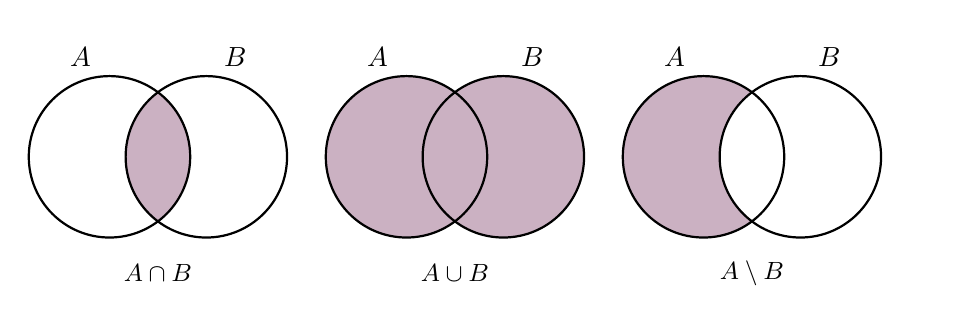
\begin{tikzpicture}[scale=0.82]
  \def\setA{(0,0) circle (1.25)}
  \def\setB{(1.5,0) circle (1.25)}
  % intersection
  \begin{scope}[shift={(0,0)}]
    \begin{scope}\clip \setA; \fill[accent!35] \setB; \end{scope}
    \draw[thick] \setA; \draw[thick] \setB;
    \node at (-0.45,1.55) {$A$}; \node at (1.95,1.55) {$B$};
    \node[font=\small] at (0.75,-1.8) {$A\cap B$};
  \end{scope}
  % union
  \begin{scope}[shift={(4.6,0)}]
    \fill[accent!35] \setA; \fill[accent!35] \setB;
    \draw[thick] \setA; \draw[thick] \setB;
    \node at (-0.45,1.55) {$A$}; \node at (1.95,1.55) {$B$};
    \node[font=\small] at (0.75,-1.8) {$A\cup B$};
  \end{scope}
  % difference
  \begin{scope}[shift={(9.2,0)}]
    \begin{scope}[even odd rule]\clip \setB (-2,-2) rectangle (3.5,2); \fill[accent!35] \setA; \end{scope}
    \draw[thick] \setA; \draw[thick] \setB;
    \node at (-0.45,1.55) {$A$}; \node at (1.95,1.55) {$B$};
    \node[font=\small] at (0.75,-1.8) {$A\setminus B$};
  \end{scope}
\end{tikzpicture}
\caption{Venn diagrams. Each circle represents a set; the shaded region is the set named below it. Left:
the intersection $A\cap B$ (in both). Centre: the union $A\cup B$ (in at least one). Right: the set
difference $A\setminus B$ (in $A$ but not in $B$), defined in \cref{sec:difference}.}
\label{fig:venn}
\end{figure}

\begin{warning}[A picture is not a proof]
Venn diagrams such as \cref{fig:venn} are excellent for seeing what a statement says and for guessing
whether it is true. They are not proofs: a proof must argue from the definitions, for an arbitrary element.
\end{warning}

\begin{example}[Preferences for fruit][ex:fruit]
Emma, Bob, Hannah and Sam like the following fruit:
\begin{align*}
E&=\{\text{oranges},\text{strawberries}\}, & B&=\{\text{oranges},\text{apples},\text{bananas}\},\\
H&=\{\text{bananas},\text{blueberries},\text{apples}\}, & S&=\{\text{bananas},\text{oranges},\text{apples},\text{blueberries}\}.
\end{align*}
Find $B\cap H$, $B\cup H$, $S\cap E$, $B\cap E$ and $E\cap H$, and decide whether $B\subseteq S$ and
$H\subseteq S$. \src{L1, slide 12}
\solution
$B\cap H$ contains the fruit that both Bob and Hannah like: $B\cap H=\{\text{apples},\text{bananas}\}$.

$B\cup H$ contains the fruit liked by at least one of them:
\[B\cup H=\{\text{oranges},\text{apples},\text{bananas},\text{blueberries}\}.\]
This is exactly $S$: as sets
(order irrelevant) the two lists contain the same four fruit, so $B\cup H=S$.

$S\cap E=\{\text{oranges}\}$ and $B\cap E=\{\text{oranges}\}$, so $S\cap E=B\cap E$.

$E\cap H=\emptyset$: Emma and Hannah have no fruit in common.

Every fruit Bob likes is liked by Sam, so $B\subseteq S$; likewise $H\subseteq S$. This also follows from
$B\cup H=S$, since every set is a subset of its union with another set. Finally, every set is a subset of
itself: $E\subseteq E$, $B\subseteq B$ and so on.
\end{example}

\begin{external}[Further algebra of $\cap$ and $\cup$]
Because $\cap$ and $\cup$ mirror ``and'' and ``or'', they obey the same laws:
\begin{itemize}
  \item associativity: $(A\cap B)\cap C=A\cap(B\cap C)$ and $(A\cup B)\cup C=A\cup(B\cup C)$;
  \item distributivity: $A\cap(B\cup C)=(A\cap B)\cup(A\cap C)$ and $A\cup(B\cap C)=(A\cup B)\cap(A\cup C)$;
  \item $A\cap B\subseteq A\subseteq A\cup B$.
\end{itemize}
Each is proved by taking an arbitrary $x$ and translating membership into ``and'' and ``or''.
\end{external}

\section{Set-builder notation}\label{sec:set-builder}

Listing elements works for small sets but not for large or infinite ones. Usually a set is described by
a property that its elements share.

\begin{definition}[Set-builder notation][def:set-builder]
Suppose that a set $A$ might contain some elements that have property $P$. Then
\[
\{x\in A\mid x\text{ has property }P\}
\]
denotes the subset of $A$ that consists of all elements of the set $A$ that have property $P$.
\src{L1, slide 13}
\end{definition}

The vertical bar is read ``such that''. The set $A$ in front of the bar says where the elements are taken
from; the condition after the bar says which of them are kept. The result is always a subset of $A$.

\begin{example}[Reading set-builder notation]
\begin{enumerate}
  \item If $A$ is the set of students at QMUL and $P$ is the property of being born after 2005, then
  $\{x\in A\mid x\text{ was born after 2005}\}$ is the set of students at QMUL who were born after 2005.
  \src{L1, slide 13}
  \item $\{n\in\N\mid n\text{ is even}\}=\{2,4,6,\dots\}$.
  \item $\{x\in\R\mid x^2<4\}$ is the set of real numbers strictly between $-2$ and $2$; in the interval
  notation of \cref{sec:intervals} it is $(-2,2)$.
  \item $\{x\in\R\mid x^2=-1\}=\emptyset$, since no real number squares to $-1$.
\end{enumerate}
\end{example}

\begin{note}[Solving is describing a set]
``Find all $x$ that satisfy $2x+1>0$'' is the same request as ``describe the set
$\{x\in\R\mid 2x+1>0\}$ more simply''. The answer $(-\tfrac12,\infty)$ in \cref{ex:lin-ineq} is a
simpler name for the same set.
\end{note}

\section{Set difference}\label{sec:difference}

\begin{definition}[Set difference][def:difference]
Given two sets $A$ and $B$, the set
\[
A\setminus B=\{x\in A\mid x\notin B\}
\]
is called the \term{difference} between sets $A$ and $B$; we also say that $A\setminus B$ is the result of
\term{subtraction} of the set $B$ from the set $A$. Thus $A\setminus B$ is the subset of elements of $A$
that are not elements of $B$. \src{L1, slide 14}
\end{definition}

\begin{example}[Set differences]
Compute
\begin{enumerate}
  \item $\{\text{apples},\text{oranges},\text{blueberries}\}\setminus\{\text{bananas},\text{oranges}\}$;
  \item $\{2,4,6,8,10,12,14,\dots\}\setminus\{3,6,9,12,15,\dots\}$.
\end{enumerate} \src{L1, slide 14}
\solution
(a) Keep the elements of the first set that are not in the second. Apples and blueberries are not in the
second set; oranges are. So the difference is $\{\text{apples},\text{blueberries}\}$. Bananas play no role:
removing something that was never there changes nothing.

(b) From the even natural numbers remove the multiples of $3$. The even numbers that are multiples of $3$
are the multiples of $6$, so we remove $6,12,18,\dots$ and are left with $\{2,4,8,10,14,16,20,\dots\}$, the
even numbers not divisible by $3$.
\end{example}

\begin{proposition}[Subset and difference][prop:subset-diff]
For sets $A$ and $B$: $A\subseteq B$ implies $A\setminus B=\emptyset$. \src{L1, slide 14} The converse is
also true, so $A\subseteq B\Leftrightarrow A\setminus B=\emptyset$.
\end{proposition}
\emph{Proof.} ($\Rightarrow$) Suppose $A\subseteq B$. An element of $A\setminus B$ would be an element of $A$
that is not in $B$; but every element of $A$ is in $B$. So $A\setminus B$ has no elements:
$A\setminus B=\emptyset$.
($\Leftarrow$) Suppose $A\setminus B=\emptyset$ and take any $x\in A$. If $x\notin B$ we would have
$x\in A\setminus B$, which is impossible; hence $x\in B$. Since $x$ was arbitrary, $A\subseteq B$.
\hfill$\square$

\begin{warning}[Set difference is not commutative]
Unlike $\cap$ and $\cup$, the order matters: in general $A\setminus B\ne B\setminus A$. For example, with
$A=\{1,2\}$ and $B=\{2,3\}$ we have $A\setminus B=\{1\}$ but $B\setminus A=\{3\}$.
\end{warning}

\begin{external}[Two useful facts about $\setminus$]
For any sets $A$ and $B$:
\begin{itemize}
  \item $A\setminus B\subseteq A$, and $A\setminus B$ has no element in common with $B$.
  \item $A\setminus B=A$ if and only if $A\cap B=\emptyset$ (removing $B$ removes nothing exactly when $A$
  and $B$ share no element).
\end{itemize}
\end{external}

\section{Sets in examination questions}\label{sec:sets-exam}

The January 2024 ECN115 paper opened with a sixteen-mark question on sets, consisting of a definition,
two ``does such a thing exist?'' parts and one ``find all'' part (as summarised in the study guide). The
following worked example reproduces that structure.

\begin{example}[Questions on set difference][ex:jan2024]
\begin{enumerate}
  \item Explain the notion of set difference $A\setminus B$.
  \item Are there non-empty sets of natural numbers $A$ and $B$ with $A\setminus B=A$? If yes, give an
  example; if no, argue why.
  \item Are there non-empty sets of natural numbers $A$ and $B$ with $A\setminus B=B$? If yes, give an
  example; if no, argue why.
  \item Find all sets $D\subseteq\N$ such that $\{1,2\}\cup D=\{1,2,3\}$.
\end{enumerate}
\src{SG: Jan 2024 Q1}
\solution
(a) For sets $A$ and $B$, $A\setminus B=\{x\in A\mid x\notin B\}$: the set of elements of $A$ that are not
elements of $B$.

(b) Yes. Take $A=\{1\}$ and $B=\{2\}$. Both are non-empty sets of natural numbers, $1\notin B$, so
$A\setminus B=\{1\}=A$. (Any two non-empty sets with no common element work.)

(c) No. Suppose $A\setminus B=B$ with $B$ non-empty, and take some $b\in B$. Then $b\in A\setminus B$, so by
the definition of set difference $b\notin B$. This contradicts $b\in B$. Hence there are no such sets. (The
argument shows more: $A\setminus B=B$ forces $B=\emptyset$.)

(d) Since $3\in\{1,2,3\}=\{1,2\}\cup D$ and $3\notin\{1,2\}$, we need $3\in D$. Since every element of $D$
lies in $\{1,2\}\cup D=\{1,2,3\}$, we need $D\subseteq\{1,2,3\}$. The elements $1$ and $2$ may or may not be
in $D$, because they are in the union anyway. Hence
\[
D\in\big\{\{3\},\ \{1,3\},\ \{2,3\},\ \{1,2,3\}\big\},
\]
four sets in all, and each of them does satisfy the condition.
\end{example}

\begin{examtip}[``If yes, give an example; if no, argue why'']
This phrasing appears on several past ECN115 papers. A ``yes'' answer needs one explicit example,
checked against every condition (including ``non-empty''). A ``no'' answer needs a general argument,
usually by contradiction: assume such objects exist and derive something impossible. Decide which it is
before writing; a quick experiment with small sets usually tells you.
\end{examtip}

\section{Sets in economics}\label{sec:sets-econ}

\begin{example}[A budget set][ex:budget-set]
A consumer with income $m=100$ buys quantities $x\ge0$ and $y\ge0$ of two goods priced $p_x=5$ and
$p_y=10$. Describe the bundles she can afford as a set, and decide whether the bundles $(10,5)$ and
$(12,5)$ are affordable.
\solution
A bundle is a pair $(x,y)$ of real numbers. The affordable bundles form the \emph{budget set}
\[
B=\{(x,y)\in\R^2\mid x\ge0,\ y\ge0,\ 5x+10y\le100\},
\]
where $\R^2$ denotes the set of all pairs of real numbers. The bundle $(10,5)$ costs $5\cdot10+10\cdot5=100$,
so $(10,5)\in B$ (it is on the budget line). The bundle $(12,5)$ costs $110>100$, so $(12,5)\notin B$.

If a rationing scheme also limits the first good to at most $8$ units, the bundles that are both
affordable and permitted form the intersection $B\cap\{(x,y)\in\R^2\mid x\le 8\}$. Each extra constraint
on a decision-maker corresponds to intersecting with one more set.
\end{example}

% --------------------------------------------------------------------
\section{Chapter review}
% --------------------------------------------------------------------
\subsection*{Summary}
A set is determined by its elements; order and repetition are irrelevant, and the empty set $\emptyset$ has
no elements. $A\subseteq B$ means every element of $A$ is in $B$; every set is a subset of itself; and two
sets are equal exactly when each is a subset of the other. Intersection ($\cap$, ``and''), union ($\cup$,
``or'') and difference ($\setminus$, ``and not'') build new sets; the first two are commutative, the third is
not. Set-builder notation $\{x\in A\mid P\}$ describes the elements of $A$ with property $P$, and solving an
equation or inequality amounts to describing such a set in simpler terms.

\subsection*{Key definitions}
\begin{itemize}
  \item $x\in A$: $x$ is an element of $A$; \ $x\notin A$: it is not.
  \item $A=B$: every element of $A$ is in $B$ and every element of $B$ is in $A$.
  \item $A\subseteq B$: every element of $A$ is in $B$ ($A$ a subset, $B$ a superset).
  \item $A\cap B$: objects in both; \ $A\cup B$: objects in $A$, in $B$ or in both.
  \item $\{x\in A\mid P\}$: elements of $A$ with property $P$.\ \ $A\setminus B=\{x\in A\mid x\notin B\}$.
\end{itemize}

\subsection*{Key facts}
\[
A=B\Leftrightarrow(A\subseteq B\text{ and }B\subseteq A),\quad A\subseteq A,\quad
A\cap B=B\cap A,\quad A\cup B=B\cup A,\quad A\subseteq B\Rightarrow A\setminus B=\emptyset.
\]

\subsection*{Connections}
Membership statements are propositions (\cref{ch:logic}), and $\cap$, $\cup$ correspond to ``and'' and
``or''. The number systems $\N,\Z,\Q,\R$ are sets, one inside the next (\cref{ch:numbers}); intervals are
subsets of $\R$ described in set-builder notation (\cref{sec:intervals}); and the solution of every
inequality in \cref{ch:ineq,ch:abs} is a set, often a union of intervals.

\subsection*{Common mistakes}
\begin{itemize}
  \item Confusing $\in$ (element of) with $\subseteq$ (subset of): $1\in\{1,2\}$ but $\{1\}\subseteq\{1,2\}$.
  \item Assuming $A\setminus B=B\setminus A$.
  \item Forgetting that ``or'' in $A\cup B$ includes elements in both sets.
  \item Treating a Venn diagram as a proof.
  \item In ``find all sets'' questions, listing only one set when several satisfy the conditions.
\end{itemize}

\subsection*{Exam checklist}
\begin{checklist}
  \item Define subset and set equality, and state $A=B\Leftrightarrow(A\subseteq B$ and $B\subseteq A)$.
  \item Define set difference in set-builder notation.
  \item Compute intersections, unions and differences of given sets.
  \item Answer ``does such a set exist?'' questions with an example or an argument by contradiction.
  \item Find all sets satisfying given union, intersection and subset conditions.
\end{checklist}

% --------------------------------------------------------------------
\section{Practice questions}
% --------------------------------------------------------------------
\pq[basic] Let $A=\{1,2,3,4,5\}$ and $B=\{4,5,6\}$. Find $A\cap B$, $A\cup B$, $A\setminus B$ and $B\setminus A$.

\pq[basic] List the elements of (a) $\{n\in\N\mid n<5\}$; (b) $\{n\in\N\mid n^2\le 30\}$;
(c) $\{x\in\R\mid x^2=4\}$; (d) $\{x\in\R\mid x^2+1=0\}$.

\pq[conceptual] Let $C=\{\{1,2\},\{1,3\},\{2,3\}\}$. Which of the following are true?
(a) $\{1,2\}\in C$; (b) $1\in C$; (c) $\{2,1\}\in C$; (d) $\{\{1,2\}\}\subseteq C$; (e) $\{1,2\}\subseteq C$.

\pq[mathematical] Prove that for any sets $A$ and $B$, $A\cap B\subseteq A$ and $A\subseteq A\cup B$.

\pq[mathematical] Prove that if $A\subseteq B$ and $B\subseteq C$, then $A\subseteq C$.

\pq[application] A firm can produce any whole number of units from $0$ to $50$ inclusive. A regulator
requires output of at least $20$ units, and capacity constraints in a second plant exclude the outputs
$30$ to $35$ inclusive. Describe the set of permitted outputs using set-builder notation and set operations,
and state how many outputs are permitted.

\pq[multi-step] Are there non-empty sets of natural numbers $A$ and $B$ such that $A\cup B=A\cap B$? If yes,
give an example and describe all such pairs; if no, argue why.

\pq[exam-style] (a) Explain what it means for a set $A$ to be a subset of a set $B$, and state what it means
for two sets to be equal in terms of subsets.
(b) Find all sets $D$ of natural numbers that satisfy both $\{2,4\}\cap D=\{2\}$ and $D\subseteq\{1,2,3,4\}$.
(c) Let $A=\{x\in\N\mid x\le10\}$ and $B=\{x\in\N\mid x\text{ is even}\}$. List the elements of $A\setminus B$
and decide whether $A\setminus B=B\setminus A$.

% --------------------------------------------------------------------
\section{Solutions to practice questions}
% --------------------------------------------------------------------
\pqsol{2.1}
$A\cap B=\{4,5\}$; $A\cup B=\{1,2,3,4,5,6\}$; $A\setminus B=\{1,2,3\}$; $B\setminus A=\{6\}$. Note that
$A\setminus B\ne B\setminus A$.

\pqsol{2.2}
(a) $\{1,2,3,4\}$ (recall $0\notin\N$). (b) $n^2\le30$ holds for $n=1,2,3,4,5$ ($5^2=25$) but not $n=6$
($36$); so $\{1,2,3,4,5\}$. (c) $\{-2,2\}$. (d) $\emptyset$.

\pqsol{2.3}
(a) True. (b) False: the elements of $C$ are sets, not numbers. (c) True: $\{2,1\}=\{1,2\}$, since order does
not matter. (d) True: the only element of $\{\{1,2\}\}$ is $\{1,2\}$, which is in $C$. (e) False: $1$ is an
element of $\{1,2\}$ but $1\notin C$.

\pqsol{2.4}
Let $x\in A\cap B$ be arbitrary. Then $x\in A$ and $x\in B$; in particular $x\in A$. So $A\cap B\subseteq A$.
Now let $x\in A$ be arbitrary. Then ``$x\in A$ or $x\in B$'' is true, so $x\in A\cup B$. So $A\subseteq A\cup B$.

\pqsol{2.5}
Let $x\in A$ be arbitrary. Since $A\subseteq B$, $x\in B$. Since $B\subseteq C$, $x\in C$. As $x$ was an
arbitrary element of $A$, $A\subseteq C$.

\pqsol{2.6}
Let $X=\{n\in\Z\mid 0\le n\le 50\}$ be the feasible outputs. The permitted outputs are
\[
\{n\in X\mid n\ge 20\}\setminus\{n\in\Z\mid 30\le n\le 35\}=\{20,21,\dots,29\}\cup\{36,37,\dots,50\}.
\]
There are $10+15=25$ permitted outputs.

\pqsol{2.7}
Yes: $A=B=\{1\}$ gives $A\cup B=\{1\}=A\cap B$. In fact this happens exactly when $A=B$. Always
$A\cap B\subseteq A\subseteq A\cup B$ (Question~2.4). If $A\cup B=A\cap B$, the outer two sets coincide, so
$A$ is squeezed between equal sets and $A=A\cap B=A\cup B$; the same argument gives $B=A\cup B$; hence
$A=B$. Conversely, if $A=B$ then $A\cup B=A=A\cap B$.

\pqsol{2.8}
(a) $A\subseteq B$ means that every element of $A$ is also an element of $B$. Two sets are equal,
$A=B$, exactly when $A\subseteq B$ and $B\subseteq A$.
(b) $\{2,4\}\cap D=\{2\}$ says $2\in D$ and $4\notin D$. $D\subseteq\{1,2,3,4\}$ says $D$ has no other elements.
So $1$ and $3$ are each free to be in or out: $D\in\{\{2\},\{1,2\},\{2,3\},\{1,2,3\}\}$.
(c) $A=\{1,\dots,10\}$, so $A\setminus B=\{1,3,5,7,9\}$. But $B\setminus A=\{12,14,16,\dots\}$, the even numbers
greater than $10$. For example $12\in B\setminus A$ while $12\notin A\setminus B$, so $A\setminus B\ne B\setminus A$.

% ====================================================================
\chapter{Number Systems and the Properties of Real Numbers}\label{ch:numbers}
% ====================================================================

\begin{chapterintro}
Economics measures prices, quantities, incomes and rates, and all of these are numbers. This chapter
introduces the four number systems used in the module --- the natural numbers, the integers, the rational
numbers and the real numbers --- and then lists the basic properties of the real numbers from which every
calculation in this book can be justified. These properties are the axioms of the module: when we solve an
inequality, every step is an application of one of them.
\end{chapterintro}

\begin{prerequisites}
Sets, subsets and set-builder notation (\cref{ch:sets}); the meaning of axiom and theorem
(\cref{sec:proof}); implication and equivalence (\cref{sec:implication,sec:equivalence}).
\end{prerequisites}

\section{The four number systems}\label{sec:number-systems}

\begin{definition}[Number systems][def:number-systems]
\begin{itemize}
  \item The \term{natural numbers} are the set $\N=\{1,2,3,\dots\}$.
  \item The \term{integers} are the set $\Z=\{\dots,-3,-2,-1,0,1,2,3,\dots\}$.
  \item The \term{rational numbers} are the set $\Q$ consisting of all numbers that can be written as $p/q$
  with $p\in\Z$ and $q\in\N$.
  \item The \term{real numbers} are (informally) the set $\R$ of points on the number line.
\end{itemize}
\src{L1, slide 16}
\end{definition}

\begin{core}[Successor property of $\N$]
For any $n\in\N$, we have $n+1\in\N$. \src{L1, slide 16}

Starting from $1$ and repeatedly adding $1$ reaches every natural number and never leaves $\N$. This simple
fact is what makes proof by induction work (\cref{ch:ind}).
\end{core}

\begin{warning}[$0$ is not a natural number in this module]
In ECN115, $\N=\{1,2,3,\dots\}$ starts at $1$. Some books include $0$. The difference matters for index
ranges in sums and for the starting point of an induction. When $0$ is wanted it is added explicitly, as in
$\{0\}\cup\N$ in the binomial formula (\cref{ch:binom}).
\end{warning}

\paragraph{Why $q\in\N$ in the definition of $\Q$} Requiring the denominator to be a natural number does
two jobs at once. It rules out $q=0$, so the fraction $p/q$ always makes sense, without a separate clause.
And it puts the sign in the numerator: $-\tfrac34$ is written $\tfrac{-3}{4}$ rather than $\tfrac{3}{-4}$.
Every rational number can be written in many ways ($\tfrac12=\tfrac24=\tfrac{50}{100}$), but this does not
matter: $\Q$ is the set of numbers that can be written in this form at least once.

\begin{proposition}[The number systems are nested][prop:nested]
\[
\N\subseteq\Z\subseteq\Q\subseteq\R. \tag*{\srcin{L1, slide 16}}
\]
\end{proposition}
Every natural number is an integer; every integer $p$ is the rational number $p/1$; and every rational
number is a point on the number line. Equality and the inequalities $\ge,\le,>,<$ are defined on all four
sets as usual, and they agree with one another: $2<3$ means the same whether $2$ and $3$ are thought of as
natural numbers or as real numbers.

\subsection{Why the real numbers are needed}
The slides note that the rational numbers are adequate for \emph{arithmetic}: adding, subtracting,
multiplying or dividing (by a non-zero number) two rational numbers always gives a rational number. The real
numbers are needed for \emph{algebra} (for example, solving $x^2=2$), \emph{geometry} (for example, the ratio of
the circumference of a circle to its diameter, $\pi$) and \emph{limits}. \src{L1, slide 16}

\begin{external}[$\sqrt2$ is not rational]
The equation $x^2=2$ has no solution in $\Q$. Suppose it did: $x=p/q$ with $p\in\Z$, $q\in\N$, and the fraction
in lowest terms (so $p$ and $q$ are not both even). Then $p^2=2q^2$, so $p^2$ is even, and therefore $p$ is even
(the square of an odd number is odd). Write $p=2k$; then $4k^2=2q^2$, so $q^2=2k^2$ is even and $q$ is even.
So $p$ and $q$ are both even, contradicting lowest terms. Hence no rational number squares to $2$. On the
number line there is nevertheless a point at distance $\sqrt2$ from $0$ (the diagonal of a unit square), so the
rational numbers have ``gaps'' that the real numbers fill. \Cref{sec:lub} describes the property of $\R$ that
captures the absence of gaps.
\end{external}

\section{The properties of the real numbers}\label{sec:axioms}

The slides list thirteen properties of the real numbers in three groups: two for the order relation, five
for addition and six for multiplication. In this module they are the axioms: we do not prove them, and every
other fact about real numbers is derived from them.

\subsection{The order relation}

\begin{definition}[Order: O1--O2][def:order]
\begin{description}[style=sameline, leftmargin=3.2em, font=\sffamily\bfseries\color{defcol}]
  \item[O1] For any real numbers $a,b$, exactly one of the following statements is true: either $a>b$, or
  $a=b$, or $a<b$.
  \begin{itemize}
    \item $a<b$ is the same as $b>a$.
    \item We write $a\ge b$ if $a>b$ or $a=b$. We write $a\le b$ if $a<b$ or $a=b$.
  \end{itemize}
  \item[O2] \emph{Transitivity:} if $a>b$ and $b>c$, then $a>c$.
\end{description}
\src{L1, slide 17}
\end{definition}

O1 is called the \term{trichotomy} property (``division into three''). It has two halves: \emph{at least}
one of the three possibilities holds, so any two real numbers can be compared; and \emph{at most} one holds,
so the possibilities exclude each other. The first half is what makes case analyses complete: when a factor
in a product is not zero, it must be positive or negative, and there is no fourth option
(\cref{ex:product-ineq}). The second half is what makes negation simple: ``not $(a>b)$'' is the same as
$a\le b$.

Note that $\ge$ and $\le$ are \emph{defined} from $>$ and $=$; they are not separate primitive notions.

\subsection{Addition}

Addition assigns to any numbers $a,b$ a unique number $a+b$.

\begin{definition}[Addition: A1--A5][def:addition]
For all real numbers $a$, $b$, $c$:
\begin{description}[style=sameline, leftmargin=3.2em, font=\sffamily\bfseries\color{defcol}]
  \item[A1] \emph{Commutativity:} $a+b=b+a$.
  \item[A2] \emph{Associativity:} $a+(b+c)=(a+b)+c$.
  \item[A3] \emph{Property of the number zero:} $a+0=a$.
  \item[A4] \emph{Existence of the additive inverse:} $a+(-a)=0$.
  \item[A5] \emph{Additivity of the order:} $a>b\ \Rightarrow\ a+c>b+c$.
\end{description}
\src{L1, slide 17}
\end{definition}

A1 and A2 say that, in a sum, neither the order of the terms nor the way they are grouped matters, which is
why we may write $a+b+c$ without brackets. A3 says that $0$ changes nothing when added. A4 says that every
number $a$ has a partner $-a$ that cancels it; subtraction is \emph{defined} by $a-b=a+(-b)$. A5 connects
addition to order: adding the same number to both sides of a strict inequality preserves it.

\begin{warning}[A5 is an implication, not an equivalence]
As stated, A5 says only $a>b\Rightarrow a+c>b+c$. The reverse direction is true but needs an argument: from
$a+c>b+c$, apply A5 again with $-c$ to get $(a+c)+(-c)>(b+c)+(-c)$, and simplify with A2--A4 to $a>b$. So
\[
a>b\quad\Longleftrightarrow\quad a+c>b+c \qquad\text{for every real } c.
\]
This is a small theorem, not the axiom itself. The slides use exactly this two-step argument in Example 1 of
\cref{ch:ineq}.
\end{warning}

\subsection{Multiplication}

Multiplication assigns to any numbers $a,b$ a unique number $a\cdot b$ (also written $ab$).

\begin{definition}[Multiplication: M1--M6][def:multiplication]
For all real numbers $a$, $b$, $c$:
\begin{description}[style=sameline, leftmargin=3.2em, font=\sffamily\bfseries\color{defcol}]
  \item[M1] \emph{Commutativity:} $a\cdot b=b\cdot a$.
  \item[M2] \emph{Associativity:} $a\cdot(b\cdot c)=(a\cdot b)\cdot c$.
  \item[M3] \emph{Properties of the number one:} $1\ne0$, and $a\cdot1=a$.
  \item[M4] \emph{Existence of the inverse of a non-zero number:} $a\cdot(1/a)=1$ for $a\ne0$.
  \item[M5] \emph{Distributive law:} $a\cdot(b+c)=a\cdot b+a\cdot c$.
  \item[M6] \emph{Multiplicative properties of the order relation:}
  \begin{itemize}
    \item if $a>b$ and $c>0$, then $a\cdot c>b\cdot c$;
    \item if $a>b$ and $c<0$, then $a\cdot c<b\cdot c$.
  \end{itemize}
\end{description}
\src{L1, slide 18}
\end{definition}

M1--M4 mirror A1--A4. Division is defined by $a/b=a\cdot(1/b)$ for $b\ne0$; there is no $1/0$, which is why
M4 carries the condition $a\ne0$. M5 is the only property that links addition and multiplication: it is what
allows brackets to be multiplied out and common factors to be taken out.

\begin{core}[M6: the sign of the multiplier decides the direction]
Multiplying both sides of an inequality by a \emph{positive} number keeps its direction; multiplying by a
\emph{negative} number reverses it. Multiplying by $0$ destroys it (both sides become $0$). Consequently:
\begin{itemize}
  \item before multiplying or dividing an inequality by anything, establish its sign;
  \item if the sign is unknown (a variable or a parameter), split into the cases positive, zero and negative.
\end{itemize}
This one habit accounts for a large share of the marks in inequality and parameter questions on past ECN115
papers.
\end{core}

\begin{note}[The rational numbers satisfy all thirteen properties]
Every one of O1--O2, A1--A5 and M1--M6 is also true in $\Q$: sums, products, negatives and reciprocals of
rational numbers are rational, and the order behaves in the same way. \src{L1, slide 19} So these properties
cannot, on their own, tell $\R$ apart from $\Q$. Whatever distinguishes the real numbers --- the existence of
$\sqrt2$, the good behaviour of limits --- must come from an additional property (\cref{sec:lub}).
\end{note}

\section{Consequences of the properties}\label{sec:consequences}

Many familiar rules of algebra are not on the list. They are theorems, derived from the list. The slides use
some of them without proof (the study guide points out that Example 2 of \cref{ch:ineq} relies on $0\cdot a=0$);
this section proves the ones needed in the book. The proofs show how theorems are built from axioms, and you
may use the results freely afterwards.

\begin{proposition}[Multiplying by zero][prop:zero-times]
For every real number $a$, $0\cdot a=0$.
\end{proposition}
\emph{Proof.} By A3, $0+0=0$. Multiply by $a$ and use M1 and M5:
$0\cdot a=(0+0)\cdot a=0\cdot a+0\cdot a$. Now add $-(0\cdot a)$ to both sides and use A2, A4 and A3:
$0=0\cdot a$. \hfill$\square$

\begin{proposition}[Zero products][prop:zero-product]
For real numbers $a,b$: if $ab=0$ then $a=0$ or $b=0$. Equivalently, if $a\ne0$ and $b\ne0$ then $ab\ne0$.
\end{proposition}
\emph{Proof.} Suppose $ab=0$ and $a\ne0$. By M4, $1/a$ exists. Then, using M2, M4, M3 and
\cref{prop:zero-times},
$b=1\cdot b=\big((1/a)\cdot a\big)\cdot b=(1/a)\cdot(ab)=(1/a)\cdot0=0$. So if $a\ne0$ then $b=0$; hence
$a=0$ or $b=0$. \hfill$\square$

\begin{proposition}[Signs][prop:signs]
For real numbers $a,b$:
\begin{enumerate}[label=(\roman*)]
  \item $(-1)\cdot a=-a$, and $-(-a)=a$;
  \item $a>0\Leftrightarrow -a<0$;
  \item $a>b\Leftrightarrow a-b>0$;
  \item if $a\ne0$ then $a^2>0$; hence $a^2\ge0$ for every $a$, and in particular $1=1^2>0$;
  \item if $a>0$ then $1/a>0$; if $a<0$ then $1/a<0$;
  \item the product of two numbers with the same sign is positive; the product of two numbers with opposite
  signs is negative.
\end{enumerate}
\end{proposition}
\emph{Proof.} (i) $a+(-1)a=1\cdot a+(-1)a=(1+(-1))a=0\cdot a=0$ by M3, M5, A4 and \cref{prop:zero-times}; so
$(-1)a$ is an additive inverse of $a$. Additive inverses are unique (if $a+b=0$ and $a+c=0$ then
$b=b+(a+c)=(b+a)+c=0+c=c$), so $(-1)a=-a$. Also $-a+a=0$ shows that $a$ is the inverse of $-a$, i.e.\ $-(-a)=a$.

(ii) If $a>0$, add $-a$ to both sides (A5): $0>-a$. Conversely, if $-a<0$, add $a$: $0<a$.

(iii) Add $-b$ to both sides of $a>b$ (A5, A4): $a-b>0$. Conversely add $b$.

(iv) If $a>0$, M6 with $c=a>0$ applied to $a>0$ gives $a\cdot a>0\cdot a=0$. If $a<0$, apply M6 to the
inequality $0>a$ with $c=a<0$: the direction reverses, giving $0\cdot a<a\cdot a$, that is, $a\cdot a>0$.
Either way $a^2>0$.

(v) Let $a>0$. By M4, $a\cdot(1/a)=1>0$. If $1/a$ were $0$ the product would be $0$; if $1/a$ were negative,
M6 applied to $a>0$ with $c=1/a<0$ would give $a\cdot(1/a)<0$. By O1, $1/a>0$. The case $a<0$ is similar.

(vi) If $a>0$ and $b>0$, M6 gives $ab>0\cdot b=0$. If $a<0$ and $b<0$, M6 with $c=b<0$ applied to $0>a$ gives
$0\cdot b<ab$, i.e.\ $ab>0$. If $a>0$ and $b<0$, M6 with $c=b<0$ applied to $a>0$ gives $ab<0$. \hfill$\square$

\begin{note}
You will not be asked to reproduce these derivations in ECN115: the slides say explicitly that, when solving
problems, ``it suffices just to do correct calculations''. They are included so that you can see that every
rule you use rests on the thirteen properties, and so that the reasoning behind sign analysis
(\cref{sec:sign-analysis}) is complete.
\end{note}

\section{The Least Upper Bound property}\label{sec:lub}

\begin{sourcenote}[Non-examinable]
The slides present this property as ``extra material, non-examinable''. It is included because it explains
\emph{why} the real numbers, rather than the rational numbers, are the right setting for limits.
\end{sourcenote}

\begin{definition}[Upper bound and least upper bound][def:lub]
Let $A\subseteq\R$ be non-empty. A number $y\in\R$ is an \term{upper bound} for $A$ if $x\le y$ for all
$x\in A$. A number $z\in\R$ is a \term{least upper bound} for $A$ if
\begin{enumerate}[label=(\roman*)]
  \item $z$ is an upper bound: $x\le z$ for all $x\in A$; and
  \item no smaller number is an upper bound: for every $w<z$ there is $x\in A$ such that $x>w$.
\end{enumerate}
\src{L1, slide 19}
\end{definition}

\begin{principle}[Least Upper Bound property][pr:lub]
If a non-empty subset $A\subseteq\R$ has an upper bound, then $A$ has a least upper bound. \src{L1, slide 19}
\end{principle}

The rational numbers do \emph{not} have this property. The set $A=\{q\in\Q\mid q>0,\ q^2<2\}$ is non-empty
($1\in A$) and bounded above (by $2$), but there is no smallest \emph{rational} upper bound: the least upper
bound would have to be $\sqrt2$, which is not rational. In $\R$ the number $\sqrt2$ exists, and it is the least
upper bound. The Least Upper Bound property is precisely the statement that the real number line has no
gaps; it is what guarantees, in Topic~3, that limits exist when we expect them to.

\section{Intervals}\label{sec:intervals}

Subsets of $\R$ consisting of all numbers between two endpoints occur so often that they have their own
notation.

\begin{definition}[Intervals][def:intervals]
For real numbers $a\le b$:
\begin{align*}
\text{closed interval:}\quad &[a,b]=\{x\in\R\mid a\le x\le b\},\\
\text{open interval:}\quad &(a,b)=\{x\in\R\mid a<x<b\},\\
\text{half-open intervals:}\quad &(a,b]=\{x\in\R\mid a<x\le b\},\qquad [a,b)=\{x\in\R\mid a\le x<b\},\\
\text{infinite intervals:}\quad &(a,\infty)=\{x\in\R\mid a<x\},\qquad (-\infty,b)=\{x\in\R\mid x<b\},\\
\text{half-infinite intervals:}\quad &[a,\infty)=\{x\in\R\mid a\le x\},\qquad (-\infty,b]=\{x\in\R\mid x\le b\},\\
&(-\infty,\infty)=\R.
\end{align*}
\src{L1, slide 20}
\end{definition}

A square bracket means the endpoint is \emph{included} ($\le$); a round bracket means it is \emph{excluded}
($<$). The symbols $\infty$ and $-\infty$ are not real numbers; they only indicate that the interval has no
upper or lower end. They can therefore never be included, and always take a round bracket.

\begin{figure}[ht]
\centering
\begin{tikzpicture}[x=9mm]
  \tikzset{open/.style={circle, draw=accent, fill=white, thick, inner sep=1.6pt},
           closed/.style={circle, draw=accent, fill=accent, thick, inner sep=1.6pt}}
  \foreach \y/\lab/\l/\r in {0/{[1,4]}/closed/closed, -0.9/{(1,4)}/open/open, -1.8/{(1,4]}/open/closed, -2.7/{[1,4)}/closed/open}{
    \draw[-{Stealth}] (-0.5,\y) -- (6.3,\y);
    \draw[accent, line width=2.2pt] (1,\y) -- (4,\y);
    \node[\l] at (1,\y) {}; \node[\r] at (4,\y) {};
    \node[anchor=west, font=\small] at (6.6,\y) {$\lab$};
  }
  \draw[-{Stealth}] (-0.5,-3.6) -- (6.3,-3.6);
  \draw[accent, line width=2.2pt, -{Stealth}] (1,-3.6) -- (6.2,-3.6);
  \node[open] at (1,-3.6) {};
  \node[anchor=west, font=\small] at (6.6,-3.6) {$(1,\infty)$};
  \draw[-{Stealth}] (-0.5,-4.5) -- (6.3,-4.5);
  \draw[accent, line width=2.2pt, {Stealth}-] (-0.4,-4.5) -- (4,-4.5);
  \node[closed] at (4,-4.5) {};
  \node[anchor=west, font=\small] at (6.6,-4.5) {$(-\infty,4]$};
  \foreach \x in {0,...,6} \draw (\x,-4.9) -- (\x,-5.05) node[below, font=\scriptsize] {\x};
\end{tikzpicture}
\caption{Intervals on the number line. A filled dot marks an included endpoint (square bracket), an open dot an
excluded endpoint (round bracket). An arrow shows that the interval continues without end.}
\label{fig:intervals}
\end{figure}

\begin{example}[Writing sets as intervals]
Write each set as an interval or a union of intervals: (a) $\{x\in\R\mid -2\le x<7\}$;
(b) $\{x\in\R\mid x>3\}$; (c) $\{x\in\R\mid x\le 0\text{ or }x>5\}$; (d) $\{x\in\R\mid x\ne 1\}$.
\solution
(a) $[-2,7)$. (b) $(3,\infty)$. (c) $(-\infty,0]\cup(5,\infty)$. (d) $(-\infty,1)\cup(1,\infty)$, which can also be
written $\R\setminus\{1\}$.
\end{example}

\begin{external}[Why the type of endpoint matters]
$[0,1)$ has a smallest element ($0$) but no largest: for any $x<1$ in the interval, $(x+1)/2$ is a larger element
of the interval. $(0,1]$ has a largest element ($1$) but no smallest. In optimisation (Topic~4) this decides
whether a function defined on the interval can attain a maximum or a minimum, which is why a question may be
posed on a half-open interval such as $(0,c]$.
\end{external}

% --------------------------------------------------------------------
\section{Chapter review}
% --------------------------------------------------------------------
\subsection*{Summary}
$\N=\{1,2,3,\dots\}$, with the successor property; $\Z$ adds zero and the negatives; $\Q$ consists of fractions
$p/q$ with $p\in\Z$, $q\in\N$; and $\R$ is, informally, the number line. They are nested:
$\N\subseteq\Z\subseteq\Q\subseteq\R$. The rationals suffice for arithmetic, but solving $x^2=2$, measuring a
circle and taking limits need $\R$. The real numbers satisfy the order properties O1 (trichotomy) and O2
(transitivity), the addition properties A1--A5 and the multiplication properties M1--M6; in ECN115 these are
the axioms. M6 --- a positive multiplier keeps an inequality, a negative one reverses it --- is the most
important for calculation. $\Q$ satisfies all thirteen properties too; the additional Least Upper Bound property
(non-examinable) is what distinguishes $\R$. Intervals name the subsets of $\R$ between two endpoints.

\subsection*{Key definitions and properties}
\begin{itemize}
  \item $\N=\{1,2,3,\dots\}$; \ $\Z=\{\dots,-1,0,1,\dots\}$; \ $\Q=\{p/q: p\in\Z,\ q\in\N\}$; \ $\R$: the number line.
  \item O1: exactly one of $a>b$, $a=b$, $a<b$. \ O2: $a>b$, $b>c\Rightarrow a>c$.
  \item A1--A4: $a+b=b+a$; $a+(b+c)=(a+b)+c$; $a+0=a$; $a+(-a)=0$. \ A5: $a>b\Rightarrow a+c>b+c$.
  \item M1--M5: $ab=ba$; $a(bc)=(ab)c$; $1\ne0$, $a\cdot1=a$; $a\cdot(1/a)=1$ $(a\ne0)$; $a(b+c)=ab+ac$.
  \item M6: $a>b$, $c>0\Rightarrow ac>bc$; \ $a>b$, $c<0\Rightarrow ac<bc$.
  \item Intervals: $[a,b]$, $(a,b)$, $(a,b]$, $[a,b)$, $(a,\infty)$, $[a,\infty)$, $(-\infty,b)$, $(-\infty,b]$, $\R$.
\end{itemize}

\subsection*{Connections}
The axioms justify every step of the inequality solving in \cref{ch:ineq}; the sign rules of
\cref{prop:signs} drive the sign analysis there. The successor property underlies induction (\cref{ch:ind}).
Intervals are the natural form of answers to inequalities and the domains of functions (\cref{ch:func}). The
Least Upper Bound property is the reason limits (\cref{ch:limits}) are studied in $\R$ rather than $\Q$.

\subsection*{Common mistakes}
\begin{itemize}
  \item Including $0$ in $\N$.
  \item Forgetting to reverse an inequality after multiplying or dividing by a negative number.
  \item Dividing by a quantity that might be zero.
  \item Putting a square bracket next to $\infty$, or the wrong bracket for a strict inequality.
  \item Assuming A5 gives an equivalence without the second step.
\end{itemize}

\subsection*{Exam checklist}
\begin{checklist}
  \item Write down $\N$, $\Z$, $\Q$, $\R$ and the inclusions between them; state the successor property.
  \item Explain why $\R$ is needed in addition to $\Q$.
  \item State O1, O2, A1--A5 and M1--M6, and say which property justifies a given step.
  \item State both clauses of M6 exactly.
  \item Write any interval in set-builder notation and vice versa.
\end{checklist}

% --------------------------------------------------------------------
\section{Practice questions}
% --------------------------------------------------------------------
\pq[basic] Decide whether each number belongs to $\N$, $\Z$, $\Q$, $\R$ (list all that apply):
$5$, $-3$, $0$, $\tfrac{-7}{2}$, $0.25$, $\sqrt9$, $\pi$.

\pq[basic] Write in set-builder notation: (a) $(-3,5]$; (b) $[2,\infty)$; (c) $(-\infty,0)\cup[1,2]$.

\pq[conceptual] Explain why the definition of $\Q$ uses $q\in\N$ rather than $q\in\Z$.

\pq[mathematical] Starting from $a>b$, and naming the property used at each step, show that $-a<-b$.

\pq[mathematical] Using the properties of the real numbers, prove that if $a>b$ and $c>d$ then $a+c>b+d$.

\pq[conceptual] Which of the thirteen properties O1--M6 fail for the natural numbers $\N$ (with the usual
addition and multiplication)? Give a reason for each.

\pq[multi-step] Let $a,b$ be real numbers with $0<a<b$. Prove that $a^2<b^2$ and that $1/a>1/b$.

\pq[exam-style] (a) State both clauses of the multiplicative property of the order relation (M6).
(b) A student argues: ``$x>y$, so multiplying both sides by $x$ gives $x^2>xy$.'' Give conditions on $x$
under which the conclusion is guaranteed, and give an example with $x>y$ for which $x^2>xy$ is false.

% --------------------------------------------------------------------
\section{Solutions to practice questions}
% --------------------------------------------------------------------
\pqsol{3.1}
$5$: $\N,\Z,\Q,\R$. \ $-3$: $\Z,\Q,\R$. \ $0$: $\Z,\Q,\R$ (not $\N$). \ $\tfrac{-7}{2}$: $\Q,\R$. \
$0.25=\tfrac14$: $\Q,\R$. \ $\sqrt9=3$: $\N,\Z,\Q,\R$. \ $\pi$: $\R$ only.

\pqsol{3.2}
(a) $\{x\in\R\mid -3<x\le5\}$. (b) $\{x\in\R\mid x\ge2\}$. (c) $\{x\in\R\mid x<0\text{ or }1\le x\le2\}$.

\pqsol{3.3}
Since $0\notin\N$, the condition $q\in\N$ excludes a zero denominator automatically, so $p/q$ is always
defined. It also fixes the sign in the numerator. With $q\in\Z$ a separate condition $q\ne0$ would be needed.

\pqsol{3.4}
Add $(-a)+(-b)$ to both sides of $a>b$ (A5): $a+((-a)+(-b))>b+((-a)+(-b))$. Rearranging with A1 and A2,
the left side is $(a+(-a))+(-b)=0+(-b)=-b$ (A4, A1, A3) and the right side is $(b+(-b))+(-a)=-a$. Hence
$-b>-a$, i.e.\ $-a<-b$. (Alternatively: multiply by $-1<0$ using M6 and \cref{prop:signs}(i).)

\pqsol{3.5}
From $a>b$, A5 with $c$ gives $a+c>b+c$. From $c>d$, A5 with $b$ gives $c+b>d+b$, i.e.\ $b+c>b+d$ (A1).
By transitivity (O2), $a+c>b+d$.

\pqsol{3.6}
A3 fails: there is no $0$ in $\N$, so ``$a+0=a$'' has no meaning inside $\N$. A4 fails: $-1\notin\N$, so $1$
has no additive inverse in $\N$. M4 fails: $2\in\N$ but $1/2\notin\N$. The order properties O1, O2, A5 and M6
(with $c\in\N$; the second clause never applies since no natural number is negative), and A1, A2, M1--M3, M5
continue to hold.

\pqsol{3.7}
Since $b>a$ and $a>0$, M6 gives $b\cdot a>a\cdot a$; since $b>a$ and $b>0$, M6 gives $b\cdot b>a\cdot b$. By M1 and
O2, $b^2>ab>a^2$. For the reciprocals: $a>0$ and $b>0$ give $ab>0$, so $1/(ab)>0$ by \cref{prop:signs}(v).
Multiply $b>a$ by $1/(ab)>0$ (M6): $b/(ab)>a/(ab)$, i.e.\ $1/a>1/b$.

\pqsol{3.8}
(a) If $a>b$ and $c>0$, then $a\cdot c>b\cdot c$. If $a>b$ and $c<0$, then $a\cdot c<b\cdot c$.
(b) The step is M6 with multiplier $x$, so it is guaranteed when $x>0$. If $x<0$ the direction reverses and
$x^2<xy$; if $x=0$ both sides are $0$. Example: $x=-1$, $y=-2$ gives $x>y$, but $x^2=1$ and $xy=2$, so
$x^2>xy$ is false.

% ====================================================================
\chapter{Solving Inequalities}\label{ch:ineq}
% ====================================================================

\begin{chapterintro}
Inequalities are everywhere in economics: a budget must not be exceeded, output cannot be negative, a
project is worth undertaking if its benefits exceed its costs. Solving an inequality means finding
\emph{every} value of the unknown for which it is true. This chapter develops the method in stages ---
linear inequalities, products of factors, quadratics and fractions --- and shows how each step rests on the
properties of the real numbers from \cref{ch:numbers}.
\end{chapterintro}

\begin{prerequisites}
Equivalence and why it matters for solving (\cref{sec:equivalence}); set-builder notation, unions and
intersections (\cref{ch:sets}); the properties O1, A1--A5 and M1--M6 and the sign rules of \cref{prop:signs}
(\cref{ch:numbers}); interval notation (\cref{sec:intervals}).
\end{prerequisites}

\section{What it means to solve an inequality}\label{sec:solve-meaning}

An inequality in an unknown $x$, such as $2x+1>0$, is a proposition depending on $x$. Its
\term{solution set} is the set of all real $x$ for which it is true, $\{x\in\R\mid 2x+1>0\}$. To
\emph{solve} the inequality is to describe this set as simply as possible, usually as an interval or a union of
intervals.

\begin{core}[Solve by a chain of equivalences]
Transform the inequality step by step, making sure that each step is an \emph{equivalence}
(\cref{sec:equivalence}). Then the final, simple inequality has exactly the same solution set as the
original, and its solution set is the answer. The two tools are:
\begin{itemize}
  \item \textbf{adding} the same number to both sides, which is always reversible (A5, applied twice);
  \item \textbf{multiplying} both sides by the same number, which is reversible if the number is
  non-zero, and which keeps the direction if the number is positive and reverses it if the number is
  negative (M6).
\end{itemize}
\end{core}

\begin{note}[How much justification to write]
The slides justify each step by naming the property used, in order to show that the methods rest on the
properties of the real numbers. They also say: ``When solving problems, it suffices just to do correct
calculations.'' \src{L1, slide 22} In your own answers you do not need to cite A5 or M4 at every line; but you
must get the direction right, and when you multiply or divide by something whose sign matters you should say
what that sign is.
\end{note}

\section{Linear inequalities}\label{sec:linear-ineq}

\begin{example}[The first inequality, step by step][ex:lin-ineq]
Find all $x$ that satisfy $2x+1>0$. \src{L1, slides 22--23}
\solution
\emph{Step 1: remove the constant.} Using A5 and A4, add the number $-1$ to both sides; then use A2--A4 to
simplify the left-hand side, and A1, A3 to find $0+(-1)=-1$:
\[
2x+1>0\ \Longrightarrow\ 2x+1+(-1)>0+(-1)\ \Longrightarrow\ 2x>-1.
\]
The reverse implication works as well: add $1$ to both sides of $2x>-1$,
\[
2x>-1\ \Longrightarrow\ 2x+1>-1+1\ \Longrightarrow\ 2x+1>0.
\]
Therefore the two inequalities are equivalent: $2x+1>0\Leftrightarrow 2x>-1$.

\emph{Step 2: remove the coefficient.} By M4 there is an inverse $1/2$ of the non-zero number $2$, and
$1/2>0$ (\cref{prop:signs}(v)). Using M6, multiply both sides of $2x>-1$ by $1/2$; the direction is kept:
\[
2x>-1\ \Longrightarrow\ \tfrac12\cdot 2x>\tfrac12\cdot(-1)\ \Longrightarrow\ x>-\tfrac12.
\]
Similarly the reverse implication holds, multiplying by $2>0$: $x>-\tfrac12\Rightarrow 2x>-1$.

\emph{Conclusion.} All three inequalities are equivalent,
\[
2x+1>0\ \Longleftrightarrow\ 2x>-1\ \Longleftrightarrow\ x>-\tfrac12,
\]
and the solution of $2x+1>0$ is $x\in(-\tfrac12,\infty)$.
\end{example}

The example shows why both directions are checked. If we had shown only $2x+1>0\Rightarrow x>-\tfrac12$, we
would know that every solution lies in $(-\tfrac12,\infty)$, but not that every number in $(-\tfrac12,\infty)$
is a solution.

\subsection{The general linear inequality}

\begin{proposition}[Solving $ax+b>0$][prop:linear]
Let $a,b\in\R$. The solution set of $ax+b>0$ is
\[
\begin{cases}
\left(-\dfrac ba,\ \infty\right) & \text{if } a>0,\\[2ex]
\left(-\infty,\ -\dfrac ba\right) & \text{if } a<0,\\[2ex]
\R\ \text{ if } b>0,\quad\text{and}\quad \emptyset\ \text{ if } b\le0, & \text{if } a=0.
\end{cases}
\]
\end{proposition}
\emph{Proof.} Adding $-b$ to both sides gives the equivalent inequality $ax>-b$. If $a>0$, multiply by
$1/a>0$, which keeps the direction: $x>-b/a$. If $a<0$, multiply by $1/a<0$, which reverses it: $x<-b/a$.
Both steps are reversible (multiply back by $a$). If $a=0$ the inequality reads $0>-b$, i.e.\ $b>0$, which does
not involve $x$ at all: it is true for every $x$ if $b>0$ and for no $x$ if $b\le0$. \hfill$\square$

\begin{example}[Dividing by a negative number]
Solve $5-3x>11$.
\solution
Add $-5$ to both sides: $-3x>6$. Now divide by $-3$, i.e.\ multiply by $-\tfrac13$. Since $-\tfrac13<0$, the
second clause of M6 applies and the direction \emph{reverses}: $x<-2$. The solution is $x\in(-\infty,-2)$.

\emph{Check.} $x=-3$ gives $5+9=14>11$, true; $x=0$ gives $5>11$, false. Both agree with the answer.
\end{example}

\begin{example}[Collecting terms first]
Find all $x$ satisfying $\tfrac12x-3>2x+1$.
\solution
Add $-2x$ and $+3$ to both sides (A5, twice): $\tfrac12x-2x>1+3$, that is, $-\tfrac32x>4$. Multiply by
$-\tfrac23<0$; the direction reverses (M6): $x<-\tfrac83$. The solution is $x\in(-\infty,-\tfrac83)$.
\emph{Check:} $x=-3$ gives $-4.5>-5$, true; $x=0$ gives $-3>1$, false. \src{SG, mock Q2(b)}
\end{example}

\subsection{Inequalities with a parameter}

A \term{parameter} is a letter standing for a fixed but unspecified number, such as a price or a tax rate.
When an inequality involves a parameter, the answer usually depends on it, and the dependence arises exactly
at the step where we multiply or divide by an expression containing it.

\begin{example}[Solving $ax>1$][ex:ax-gt-1]
Let $a\in\R$ be a parameter. Find all $x$ with $ax>1$.
\solution
The step we would like to take is ``divide by $a$''. Whether this is allowed, and what it does to the
direction, depends on the sign of $a$, so we split into three exhaustive cases (O1).
\begin{itemize}
  \item $a>0$: $1/a$ exists (M4) and is positive, so the direction is kept: $x>1/a$, i.e.\ $x\in(1/a,\infty)$.
  \item $a<0$: $1/a$ exists and is negative, so the direction reverses: $x<1/a$, i.e.\ $x\in(-\infty,1/a)$.
  \item $a=0$: there is no $1/0$, so we cannot divide. The inequality reads $0>1$, false for every $x$: the
  solution set is $\emptyset$.
\end{itemize}
\end{example}

\begin{example}[A parameter multiplying a bracket]
Let $a\in\R$. Find all $x$ satisfying $a(x-1)>0$. \src{SG, mock Q2(d)}
\solution
\begin{itemize}
  \item $a>0$: multiply by $1/a>0$: $x-1>0$, so $x\in(1,\infty)$.
  \item $a<0$: multiply by $1/a<0$, reversing: $x-1<0$, so $x\in(-\infty,1)$.
  \item $a=0$: the left side is $0$ for every $x$, and $0>0$ is false, so the solution set is $\emptyset$.
\end{itemize}
\end{example}

\begin{examtip}[``Your answer should depend on the parameter'']
Parameter questions appeared on all three past ECN115 papers summarised in the study guide, usually with a
hint such as ``consider three cases: $a>0$, $a=0$, $a<0$''. The marks are for carrying out each case correctly
and for not forgetting the case $a=0$, which can never be folded into the other two because $1/0$ does not
exist.
\end{examtip}

\section{Products: sign analysis}\label{sec:sign-analysis}

\begin{example}[A product of two linear factors][ex:product-ineq]
Find all $x$ that satisfy $(2x+1)(x-1)>0$. \src{L1, slide 24}
\solution
Neither $2x+1$ nor $x-1$ can be equal to zero: otherwise $(2x+1)(x-1)=0$ (\cref{prop:zero-times}), and $0>0$
is false. So by trichotomy (O1) each factor is either positive or negative, and it suffices to consider four
cases (\cref{prop:signs}(vi)):
\begin{center}
\begin{tabular}{ccc}
\toprule
$2x+1$ & $x-1$ & $(2x+1)(x-1)$\\
\midrule
$>0$ & $>0$ & $>0$\\
$>0$ & $<0$ & $<0$\\
$<0$ & $>0$ & $<0$\\
$<0$ & $<0$ & $>0$\\
\bottomrule
\end{tabular}
\end{center}
Therefore $(2x+1)(x-1)>0$ if and only if
\[
\big[\,2x+1>0\ \text{ and }\ x-1>0\,\big]\quad\text{or}\quad\big[\,2x+1<0\ \text{ and }\ x-1<0\,\big].
\]
Since $2x+1>0$ is equivalent to $x>-\tfrac12$, $x-1>0$ is equivalent to $x>1$, and $x>1\Rightarrow x>-\tfrac12$,
we have $[2x+1>0\text{ and }x-1>0]\Leftrightarrow x>1$. Similarly $[2x+1<0\text{ and }x-1<0]\Leftrightarrow x<-\tfrac12$.
Thus the solution is
\[
x\in(-\infty,-\tfrac12)\cup(1,\infty).
\]
\end{example}

Two small but important points of logic appear in this example. Inside each case the two conditions are joined
by ``and'', so their solution sets are \emph{intersected}; and a pair of conditions such as ``$x>1$ and
$x>-\tfrac12$'' collapses to the stronger one, $x>1$. The cases themselves are joined by ``or'', so their
solution sets are combined by \emph{union}.

\subsection{The sign chart}

The four-case table can be organised on the number line. The \term{critical points} are the values where a
factor is zero, here $x=-\tfrac12$ and $x=1$. They split the line into intervals, and on each interval every
factor keeps one sign. Record the signs in a chart and multiply.

\begin{figure}[ht]
\centering
\begin{tikzpicture}[x=11mm, y=7mm]
  \draw[-{Stealth}] (-3.5,0) -- (4.5,0) node[right] {$x$};
  \foreach \x/\l in {-1/{-\tfrac12}, 2/{1}} { \draw (\x,0.15) -- (\x,-0.15) node[below] {$\l$}; }
  \node[anchor=east, font=\small] at (-3.6,-1.3) {$2x+1$};
  \node[anchor=east, font=\small] at (-3.6,-2.3) {$x-1$};
  \node[anchor=east, font=\small] at (-3.6,-3.3) {$(2x+1)(x-1)$};
  \foreach \y/\a/\b/\c in {-1.3/$-$/$+$/$+$, -2.3/$-$/$-$/$+$, -3.3/$+$/$-$/$+$} {
    \node at (-2.4,\y) {\a}; \node at (0.5,\y) {\b}; \node at (3.3,\y) {\c};
  }
  \foreach \x in {-1,2} \draw[guide] (\x,-0.4) -- (\x,-3.8);
  \node[font=\small] at (-1,-1.3) {$0$}; \node[font=\small] at (2,-2.3) {$0$};
  \node[font=\small] at (-1,-3.3) {$0$}; \node[font=\small] at (2,-3.3) {$0$};
  \draw[accent, line width=2.4pt] (-3.4,-4.4) -- (-1,-4.4); \draw[accent, line width=2.4pt] (2,-4.4) -- (4.4,-4.4);
  \node[circle, draw=accent, fill=white, thick, inner sep=1.5pt] at (-1,-4.4) {};
  \node[circle, draw=accent, fill=white, thick, inner sep=1.5pt] at (2,-4.4) {};
  \node[anchor=east, font=\small] at (-3.6,-4.4) {solution of $>0$};
\end{tikzpicture}
\caption{Sign chart for $(2x+1)(x-1)$. The critical points $-\tfrac12$ and $1$ divide the line into three
intervals; on each, each factor has a constant sign. The product is positive on the two outer intervals, so
the solution of $(2x+1)(x-1)>0$ is $(-\infty,-\tfrac12)\cup(1,\infty)$. Open dots show that the critical points
are excluded, because the inequality is strict.}
\label{fig:sign-chart}
\end{figure}

\begin{external}[Why the signs are constant between critical points]
A linear factor $mx+c$ with $m\ne0$ changes sign only at its root $-c/m$: by \cref{prop:linear} it is positive on
one side of the root and negative on the other. So between consecutive critical points no factor changes sign,
and neither does the product. This is why testing one convenient point in each interval is enough.
\end{external}

\begin{example}[A product that must be negative]
Solve $(x+3)(2x-7)<0$.
\solution
The critical points are $x=-3$ and $x=\tfrac72$. A product is negative exactly when the factors have opposite
signs:
\begin{itemize}
  \item $x+3>0$ and $2x-7<0$: $x>-3$ and $x<\tfrac72$, i.e.\ $-3<x<\tfrac72$;
  \item $x+3<0$ and $2x-7>0$: $x<-3$ and $x>\tfrac72$, which is impossible.
\end{itemize}
The solution is $x\in(-3,\tfrac72)$.
\end{example}

\begin{example}[A non-strict inequality][ex:nonstrict]
Find all $x$ satisfying $(3-x)(x+2)\ge0$. \src{SG, mock Q2(c)}
\solution
Now the product may also be \emph{zero}, which happens at $x=3$ and $x=-2$; both satisfy $\ge0$, so they are
included. Away from these points each factor is positive or negative, and the product is positive when the signs
agree:
\begin{itemize}
  \item $3-x>0$ and $x+2>0$: $x<3$ and $x>-2$, i.e.\ $-2<x<3$;
  \item $3-x<0$ and $x+2<0$: $x>3$ and $x<-2$, impossible.
\end{itemize}
Adding the two points where the product is zero gives $x\in[-2,3]$. Note the \emph{square} brackets.
\end{example}

\begin{warning}[Strict and non-strict inequalities]
For $>0$ or $<0$ the critical points are excluded (round brackets); for $\ge0$ or $\le0$ they are included
(square brackets). Writing $(-2,3)$ instead of $[-2,3]$ in \cref{ex:nonstrict} omits two solutions.
\end{warning}

\section{Quadratic inequalities}\label{sec:quadratic}

A quadratic inequality, such as $3x^2-5x+2>0$, can be solved by rewriting the quadratic as a product of two
linear factors and then using sign analysis.

\begin{example}[Factorising through the roots][ex:quad-ineq]
Find all $x$ that satisfy $3x^2-5x+2>0$. \src{L1, slide 25}
\solution
\emph{Idea.} Represent $3x^2-5x+2$ as a product of two linear terms (if possible),
$3x^2-5x+2=e\cdot(x+f)\cdot(x+g)$ for some real numbers $e,f,g$.

\emph{Finding $e$.} Expanding, $e(x+f)(x+g)=ex^2+e(f+g)x+efg$. Comparing the coefficients of $x^2$ gives $e=3$.
Comparing the others gives only $f+g=-\tfrac53$ and $fg=\tfrac23$, which do not immediately give $f$ and $g$.

\emph{Observation.} Substitute $x=-f$: then $e(x+f)(x+g)=e\cdot0\cdot(g-f)=0$. Thus $x=-f$ is a solution
(\emph{root}) of the equation $3x^2-5x+2=0$, and similarly $x=-g$ is a root. So $f$ and $g$ can be found by
solving the equation.

\emph{Solving the equation.} The discriminant is $D=(-5)^2-4\cdot3\cdot2=25-24=1$, so the roots are
\[
x_{1,2}=\frac{-(-5)\pm\sqrt1}{2\cdot 3}=\frac{5\pm1}{6},\qquad x_1=\tfrac23,\quad x_2=1.
\]
Hence $3x^2-5x+2=3\,(x-\tfrac23)(x-1)$.

\emph{Sign analysis.} Solving $3(x-\tfrac23)(x-1)>0$ as in \cref{ex:product-ineq} (the factor $3$ is positive and
does not affect the sign), the inequality $3x^2-5x+2>0$ is equivalent to
\[
x\in(-\infty,\tfrac23)\cup(1,\infty).
\]
\end{example}

\subsection{The quadratic formula}

\begin{keyformula}[Roots of a quadratic][kf:quadratic]{x_{1,2}=\frac{-b\pm\sqrt{D}}{2a},\qquad D=b^2-4ac}
\fsymbols $a,b,c$ are the real coefficients of $ax^2+bx+c$, with $a\ne0$; $D$ is the \emph{discriminant};
$x_1,x_2$ are the roots, the values of $x$ where $ax^2+bx+c=0$; the symbol $\pm$ means that one root uses $+$
and the other $-$.
\fmeaning The formula gives every real solution of $ax^2+bx+c=0$. The discriminant tells you how many there are:
two distinct real roots if $D>0$, one repeated root $x=-b/(2a)$ if $D=0$, and no real roots if $D<0$ (the square
root of a negative number is not a real number).
\forigin Completing the square: $ax^2+bx+c=a\big[(x+\tfrac b{2a})^2-\tfrac{D}{4a^2}\big]$ (\cref{kf:complete-square}).
Setting this to zero gives $(x+\tfrac b{2a})^2=\tfrac D{4a^2}$, and taking square roots (possible only when $D\ge0$)
gives the formula.
\fuse Whenever a quadratic must be factorised and the factors are not obvious; in particular, as the first step in
solving any quadratic inequality.
\fexample For $3x^2-5x+2$: $a=3$, $b=-5$, $c=2$. Then $D=(-5)^2-4(3)(2)=1$, $\sqrt D=1$, and
$x=\frac{5\pm1}{6}$, giving $\tfrac23$ and $1$. Check: $3(\tfrac23)^2-5(\tfrac23)+2=\tfrac43-\tfrac{10}3+2=0$.
\fmistakes Writing $-b$ incorrectly when $b$ is negative (here $-b=+5$); dividing only $\sqrt D$ by $2a$ instead
of the whole numerator; forgetting that $D<0$ means there are no real roots, not that the formula ``fails''.
\frearrange Once the roots are known, the quadratic factorises as
$ax^2+bx+c=a(x-x_1)(x-x_2)$. Comparing coefficients gives $x_1+x_2=-b/a$ and $x_1x_2=c/a$, a quick check on
the roots.
\fchanges Increasing $c$ (with $a>0$) lowers $D=b^2-4ac$: the two roots move towards each other, merge when
$D=0$, and disappear when $D<0$. Geometrically the parabola is lifted upwards until it no longer meets the
$x$-axis.
\fexam Usually as an unmarked first step (``factorise'', ``find the roots''). A parameter in $c$ leads to a question
such as ``for which values of $c$ does the equation have two distinct roots?'', answered by solving $D>0$.
\end{keyformula}

\subsection{The sign of a quadratic}

Once $ax^2+bx+c=a(x-x_1)(x-x_2)$ with $x_1<x_2$, sign analysis gives a rule worth remembering.

\begin{proposition}[Sign of a quadratic with two roots][prop:quad-sign]
Let $a>0$ and $x_1<x_2$. Then $a(x-x_1)(x-x_2)$ is positive for $x<x_1$ and for $x>x_2$, zero at $x_1$ and $x_2$,
and negative for $x_1<x<x_2$. If $a<0$ all the signs are reversed.
\end{proposition}
\emph{Proof.} For $x<x_1$ both factors are negative; for $x>x_2$ both are positive; between the roots
$x-x_1>0$ and $x-x_2<0$. Apply \cref{prop:signs}(vi), then multiply by $a$ using M6. \hfill$\square$

\begin{figure}[ht]
\centering
\begin{tikzpicture}
\begin{axis}[stat, width=9cm, height=6.2cm, xmin=-0.6, xmax=2.2, ymin=-0.6, ymax=3.2,
  xlabel={$x$}, ylabel={$y$}, xtick={0,0.6667,1,2}, xticklabels={$0$,$\tfrac23$,$1$,$2$},
  ytick={0,1,2,3}, axis x line=middle, axis y line=middle, x label style={anchor=west}, y label style={anchor=south}]
  \addplot[curve, accent, domain=-0.45:2.05, samples=100] {3*x^2-5*x+2};
  \addplot[line width=3pt, corecol, opacity=0.8, domain=-0.6:0.6667] {0};
  \addplot[line width=3pt, corecol, opacity=0.8, domain=1:2.2] {0};
  \node[circle, draw=corecol, fill=white, thick, inner sep=1.5pt] at (axis cs:0.6667,0) {};
  \node[circle, draw=corecol, fill=white, thick, inner sep=1.5pt] at (axis cs:1,0) {};
  \node[lab, accent, anchor=west] at (axis cs:0.15,2.6) {$y=3x^2-5x+2$};
\end{axis}
\end{tikzpicture}
\caption{The parabola $y=3x^2-5x+2$ opens upwards because the leading coefficient $3$ is positive. It crosses the
$x$-axis at the roots $\tfrac23$ and $1$, lies below the axis between them and above it outside them. The thick
segments show the solution set of $3x^2-5x+2>0$.}
\label{fig:parabola}
\end{figure}

\begin{warning}[Answering between the roots]
For a quadratic with positive leading coefficient, ``$>0$'' is solved \emph{outside} the roots and ``$<0$''
\emph{between} them. A quick test of one point (for example $x=0$, if it is not a root) catches the error: in
\cref{ex:quad-ineq}, $x=0$ gives $2>0$, and $0$ is indeed outside $[\tfrac23,1]$.
\end{warning}

\subsection{When the discriminant is zero or negative}

The lecture example has $D>0$. The other two cases are handled by completing the square.

\begin{keyformula}[Completing the square][kf:complete-square]{ax^2+bx+c=a\left(x+\frac{b}{2a}\right)^2-\frac{D}{4a},\qquad D=b^2-4ac}
\fsymbols $a\ne0$, $b$, $c$ real coefficients; $D$ the discriminant.
\fmeaning Every quadratic is a multiple of a perfect square plus a constant. Since a square is never negative, the
sign of the quadratic can be read off directly.
\forigin Expand the right-hand side:
$a\big(x^2+\tfrac bax+\tfrac{b^2}{4a^2}\big)-\tfrac{b^2-4ac}{4a}=ax^2+bx+\tfrac{b^2}{4a}-\tfrac{b^2}{4a}+c=ax^2+bx+c$.
\fuse When $D=0$ or $D<0$, or when you need the minimum (or maximum) value of a quadratic.
\fexample $x^2-5x+\tfrac{25}{4}=(x-\tfrac52)^2$ ($D=0$), and $x^2-5x+7=(x-\tfrac52)^2+\tfrac34$ ($D=-3$).
\fmistakes Forgetting to factor out $a$ before completing the square; sign errors in $\tfrac b{2a}$.
\fchanges If $a>0$ the quadratic is smallest at $x=-\tfrac b{2a}$, where it equals $-\tfrac D{4a}$. If $D<0$ this
minimum is positive, so the quadratic is positive everywhere; if $D=0$ the minimum is $0$, attained only at
$x=-\tfrac b{2a}$.
\fexam ``Show that the expression is positive for all $x$'', with the hint ``write it as a square plus a constant''.
\end{keyformula}

\begin{proposition}[Sign of a quadratic when $D\le0$][prop:quad-D0]
Let $a>0$. If $D=0$, then $ax^2+bx+c=a(x-x_0)^2$ with $x_0=-\tfrac b{2a}$, which is positive for every
$x\ne x_0$ and zero at $x_0$. If $D<0$, then $ax^2+bx+c>0$ for every real $x$.
\end{proposition}
\emph{Proof.} By \cref{kf:complete-square}, $ax^2+bx+c=a(x-x_0)^2-\tfrac D{4a}$. A square is $\ge0$, and is $>0$
unless what is squared is zero (\cref{prop:signs}(iv)). If $D=0$ the constant vanishes; if $D<0$ the constant
$-\tfrac D{4a}$ is positive, so the sum is positive. \hfill$\square$

\begin{example}[A quadratic with a parameter][ex:quad-param]
Let $c\in\R$ and consider $x^2-5x+c$. \src{SG, mock Q3}
\begin{enumerate}
  \item For which $c$ does $x^2-5x+c=0$ have two distinct real roots?
  \item Solve $x^2-5x+6>0$.
  \item Solve $x^2-5x+\tfrac{25}4>0$.
  \item Show that if $c>\tfrac{25}{4}$ then $x^2-5x+c>0$ for every $x\in\R$.
\end{enumerate}
\solution
(a) $D=(-5)^2-4\cdot1\cdot c=25-4c$. Two distinct roots exactly when $D>0$: $25-4c>0\Leftrightarrow c<\tfrac{25}4$
(dividing by $4>0$ keeps the direction). So $c\in(-\infty,\tfrac{25}4)$.

(b) $D=1$, roots $\frac{5\pm1}2=2,3$, so $x^2-5x+6=(x-2)(x-3)$. The leading coefficient is positive, so the
expression is positive outside the roots: $x\in(-\infty,2)\cup(3,\infty)$.

(c) $D=0$ and $x^2-5x+\tfrac{25}4=(x-\tfrac52)^2$, which is positive except at $x=\tfrac52$. So
$x\in(-\infty,\tfrac52)\cup(\tfrac52,\infty)=\R\setminus\{\tfrac52\}$. In (b) a whole interval was excluded; here
the two roots have merged and only one point is excluded.

(d) Completing the square, $x^2-5x+c=(x-\tfrac52)^2+(c-\tfrac{25}4)$. The square is $\ge0$ and, when
$c>\tfrac{25}4$, the constant is $>0$; so the sum is positive for every $x$. (This is the case $D<0$.)
\end{example}

\begin{example}[A non-strict quadratic inequality]
Solve $2x^2-7x+3\ge0$.
\solution
$D=49-24=25$, roots $\frac{7\pm5}{4}$, i.e.\ $\tfrac12$ and $3$. So $2x^2-7x+3=2(x-\tfrac12)(x-3)$. With leading
coefficient $2>0$, the expression is $\ge0$ outside the roots and at the roots themselves:
$x\in(-\infty,\tfrac12]\cup[3,\infty)$.
\end{example}

\section{Inequalities involving fractions}\label{sec:fraction-ineq}

\begin{example}[An incorrect argument][ex:one-over-x]
A student solves $\dfrac1x>2$ as follows: ``Multiply both sides by $x$ to obtain $1>2x$. Dividing by $2$ gives
$x<\tfrac12$. Therefore the solution is $x\in(-\infty,\tfrac12)$.'' Explain the error and find the correct
solution. \src{SG, mock Q6}
\solution
\emph{The error.} Multiplying an inequality by $x$ is governed by M6, which keeps the direction only if $x>0$ and
reverses it if $x<0$. The sign of $x$ is unknown, so the step is not justified. Moreover $x=0$ is not allowed at
all, since $1/0$ is undefined.

\emph{A value wrongly included.} $x=-1$ lies in the student's answer, but $1/(-1)=-1>2$ is false.

\emph{Correct solution.} Split by the sign of $x$.
\begin{itemize}
  \item $x>0$: multiplying by $x>0$ keeps the direction, $1>2x$, so $x<\tfrac12$. With $x>0$: $0<x<\tfrac12$.
  \item $x<0$: then $1/x<0<2$ (\cref{prop:signs}(v)), so the inequality fails for every negative $x$.
  \item $x=0$: excluded, as $1/x$ is undefined.
\end{itemize}
The solution set is $(0,\tfrac12)$.
\end{example}

The safest general method avoids multiplying by an expression of unknown sign altogether.

\begin{core}[Method for inequalities with fractions]
\begin{enumerate}[label=\arabic*.]
  \item Move everything to one side, so that the other side is $0$.
  \item Combine into a single fraction $\dfrac{N(x)}{M(x)}$ and factorise numerator and denominator.
  \item Apply sign analysis to the factors of $N$ and $M$: a quotient has the same sign as the corresponding
  product, because $N/M=N\cdot M\cdot(1/M^2)$ and $1/M^2>0$.
  \item Exclude the zeros of $M$ (the fraction is undefined there); include the zeros of $N$ only for
  $\ge$ or $\le$.
\end{enumerate}
\end{core}

\begin{example}[Using the method]
Solve $\dfrac1x>2$ and $\dfrac{x+1}{x-2}\ge0$.
\solution
For the first, $\frac1x-2>0\Leftrightarrow\frac{1-2x}{x}>0$. Critical points $x=0$ and $x=\tfrac12$. Signs:
for $x<0$, numerator $+$, denominator $-$, quotient $-$; for $0<x<\tfrac12$, both $+$, quotient $+$; for
$x>\tfrac12$, numerator $-$, denominator $+$, quotient $-$. Solution $(0,\tfrac12)$, as before.

For the second, critical points $x=-1$ (numerator zero) and $x=2$ (denominator zero). For $x<-1$ both factors
are negative, quotient positive; for $-1<x<2$ the quotient is negative; for $x>2$ it is positive. Include $x=-1$
(where the quotient is $0$) but not $x=2$ (undefined): $x\in(-\infty,-1]\cup(2,\infty)$.
\end{example}

\section{Inequalities in economics}\label{sec:ineq-econ}

\begin{example}[Break-even output][ex:break-even]
A firm sells its product at price $p=12$ per unit. Its total cost of producing $q$ units is $C(q)=200+7q$
(a fixed cost of $200$ and a cost of $7$ per unit). For which outputs $q\ge0$ does the firm make a strictly
positive profit?
\solution
Profit is revenue minus cost: $\pi(q)=12q-(200+7q)=5q-200$. We need $5q-200>0\Leftrightarrow 5q>200\Leftrightarrow q>40$
(multiplying by $\tfrac15>0$). The firm makes a profit exactly when $q\in(40,\infty)$. The value $q=40$ is the
\emph{break-even output}.
\end{example}

\begin{example}[A quadratic profit function]
Suppose instead that profit is $\pi(q)=-q^2+10q-16$. For which $q$ is profit positive?
\solution
$-q^2+10q-16>0\Leftrightarrow q^2-10q+16<0$ (multiplying by $-1$ reverses the direction). The roots of
$q^2-10q+16$ are $\frac{10\pm\sqrt{100-64}}2=\frac{10\pm6}2$, i.e.\ $2$ and $8$, so $q^2-10q+16=(q-2)(q-8)$, which is
negative between the roots. Profit is positive exactly for $q\in(2,8)$: producing too little fails to cover
fixed costs, and producing too much drives costs up faster than revenue.
\end{example}

% --------------------------------------------------------------------
\section{Chapter review}
% --------------------------------------------------------------------
\subsection*{Summary}
Solving an inequality means describing its solution set exactly, which requires a chain of equivalences.
Adding a number to both sides is always reversible; multiplying by a positive number keeps the direction,
by a negative number reverses it, and by zero destroys it (M6). A linear inequality $ax+b>0$ is solved by one
addition and one multiplication, with three cases when $a$ is a parameter. A product is positive when its
factors share a sign and negative when they have opposite signs; organising this on the number line around the
critical points gives the sign chart. A quadratic is factorised through its roots, found with the discriminant;
with positive leading coefficient it is positive outside its roots and negative between them, and completing the
square handles the cases $D=0$ and $D<0$. Fractions are handled by moving everything to one side and analysing
the signs of numerator and denominator, never by multiplying by an expression of unknown sign.

\subsection*{Key definitions}
\begin{itemize}
  \item \textbf{Solution set} of an inequality: the set of all values of the unknown for which it is true.
  \item \textbf{Critical points}: the values at which a factor (of a numerator or denominator) is zero.
  \item \textbf{Discriminant} of $ax^2+bx+c$: $D=b^2-4ac$.
\end{itemize}

\subsection*{Key equations}
\begin{gather*}
D=b^2-4ac,\qquad x_{1,2}=\frac{-b\pm\sqrt D}{2a},\\
ax^2+bx+c=a(x-x_1)(x-x_2)\ \ (D\ge0),\qquad
ax^2+bx+c=a\Big(x+\frac b{2a}\Big)^2-\frac D{4a}.
\end{gather*}

\subsection*{Connections}
Every step uses the properties of \cref{ch:numbers}. Answers are sets, written with the interval and union
notation of \cref{ch:sets}. Absolute-value inequalities (\cref{ch:abs}) reduce to the methods here, and the
definition of a limit (\cref{ch:limits}) requires solving inequalities such as $2^{-n}<\varepsilon$ for $n$.
In Topic~4, the sign of a derivative written as a fraction $P(x)/Q(x)$ is found by exactly this sign analysis.

\subsection*{Common mistakes}
\begin{itemize}
  \item Not reversing the inequality when multiplying or dividing by a negative number.
  \item Dividing by a parameter or variable without considering its sign, or forgetting the zero case.
  \item Multiplying both sides by $x$ in an inequality with $1/x$.
  \item Using $\cap$ to combine the cases of a sign analysis (cases are combined with $\cup$).
  \item Solving ``$>0$'' for a quadratic with positive leading coefficient by taking the interval between the roots.
  \item Wrong brackets: round for strict inequalities and for excluded points, square for included endpoints.
\end{itemize}

\subsection*{Exam checklist}
\begin{checklist}
  \item Solve a linear inequality, stating where the direction changes and why.
  \item Solve $ax>b$ or $a(x-k)>0$ for all values of a parameter $a$.
  \item Carry out a sign analysis for a product of linear factors, including non-strict cases.
  \item Find roots with the discriminant and factorise a quadratic.
  \item Solve quadratic inequalities for $D>0$, $D=0$ and $D<0$.
  \item Solve inequalities involving fractions without multiplying by an expression of unknown sign.
\end{checklist}

% --------------------------------------------------------------------
\section{Practice questions}
% --------------------------------------------------------------------
\pq[basic] Solve: (a) $3x-4\le 8$; (b) $7-2x>1$; (c) $\tfrac{x}{3}+1\ge \tfrac{x}{2}$.

\pq[basic] Solve $(x-4)(x+1)>0$ and $(x-4)(x+1)\le0$.

\pq[mathematical] Solve $x^2-x-6<0$ and $4x^2+4x+1>0$.

\pq[mathematical] Show that $x^2+2x+5>0$ for every real $x$.

\pq[conceptual] Explain why, in a sign analysis, the cases are combined with $\cup$ while the conditions within a
case are combined with $\cap$.

\pq[mathematical] Solve $\dfrac{2x-1}{x+3}<1$.

\pq[application] A consumer has $\pounds 60$ to spend on two goods priced $\pounds 4$ and $\pounds 6$ per unit. She
wants to buy $x$ units of the first good and exactly $6$ units of the second. For which $x\ge0$ can she afford
this?

\pq[multi-step] Let $b\in\R$ be a parameter. Find all $x$ with $bx+3>x$. Your answer should depend on $b$.

\pq[multi-step] For which values of the parameter $k$ is $x^2+kx+4>0$ for every real $x$?

\pq[exam-style] Let $a\in\R$ be a parameter.
(a) Find all $x$ satisfying $(x-a)(x-1)<0$. Your answer should depend on $a$. Hint: consider the cases $a>1$,
$a=1$ and $a<1$.
(b) A student claims that $\dfrac{x-1}{x}\ge1$ is equivalent to $x-1\ge x$ and hence has no solutions. Explain
why the argument is not correct and find the solution set.

% --------------------------------------------------------------------
\section{Solutions to practice questions}
% --------------------------------------------------------------------
\pqsol{4.1}
(a) $3x\le12$, so $x\le4$: $x\in(-\infty,4]$.
(b) $-2x>-6$; dividing by $-2<0$ reverses: $x<3$, so $x\in(-\infty,3)$.
(c) Multiply by $6>0$: $2x+6\ge3x$, so $6\ge x$: $x\in(-\infty,6]$.

\pqsol{4.2}
Critical points $-1$ and $4$. The product is positive when both factors have the same sign: $x<-1$ or $x>4$. So
$(x-4)(x+1)>0\Leftrightarrow x\in(-\infty,-1)\cup(4,\infty)$, and $(x-4)(x+1)\le0\Leftrightarrow x\in[-1,4]$
(between the roots, roots included).

\pqsol{4.3}
$x^2-x-6=(x-3)(x+2)$, negative between the roots: $x\in(-2,3)$.
$4x^2+4x+1=(2x+1)^2$ ($D=0$), positive except at $x=-\tfrac12$: $x\in\R\setminus\{-\tfrac12\}$.

\pqsol{4.4}
$x^2+2x+5=(x+1)^2+4$. A square is $\ge0$, so the sum is $\ge4>0$ for every $x$. (Equivalently $D=4-20<0$ with a
positive leading coefficient.)

\pqsol{4.5}
Within a case, \emph{both} conditions must hold (for instance ``$2x+1>0$ \emph{and} $x-1>0$''), and the set of $x$
satisfying two conditions simultaneously is the intersection of their solution sets. A number solves the
original inequality if it falls into \emph{some} case (``case 1 \emph{or} case 4''), and the set of $x$ satisfying
at least one of several conditions is the union of their solution sets. Intersection corresponds to ``and'' and
union to ``or'' (\cref{sec:intersection-union}).

\pqsol{4.6}
$\frac{2x-1}{x+3}-1<0\Leftrightarrow\frac{2x-1-(x+3)}{x+3}<0\Leftrightarrow\frac{x-4}{x+3}<0$. Critical points
$-3$ and $4$; the quotient is negative when the signs differ, which happens for $-3<x<4$. Solution $(-3,4)$.

\pqsol{4.7}
Cost $4x+6\cdot6=4x+36\le60\Leftrightarrow4x\le24\Leftrightarrow x\le6$. With $x\ge0$: $x\in[0,6]$.

\pqsol{4.8}
$bx+3>x\Leftrightarrow(b-1)x>-3$.
If $b>1$: $x>-\frac3{b-1}$, i.e.\ $x\in\big(-\frac3{b-1},\infty\big)$.
If $b<1$: dividing by $b-1<0$ reverses, $x<-\frac3{b-1}=\frac3{1-b}$, i.e.\ $x\in\big(-\infty,\frac3{1-b}\big)$.
If $b=1$: $0>-3$, true for all $x$: the solution set is $\R$.

\pqsol{4.9}
With leading coefficient $1>0$, $x^2+kx+4>0$ for all $x$ exactly when there are no real roots, $D<0$ (if $D=0$
the quadratic is zero at one point; if $D>0$ it is negative between the roots). $D=k^2-16<0\Leftrightarrow
(k-4)(k+4)<0\Leftrightarrow k\in(-4,4)$.

\pqsol{4.10}
(a) The critical points are $a$ and $1$; the product is negative strictly between them.
If $a>1$: $x\in(1,a)$. If $a<1$: $x\in(a,1)$. If $a=1$: $(x-1)^2<0$ has no solution, so the solution set is
$\emptyset$.
(b) Multiplying by $x$ is valid only for $x>0$; for $x<0$ the direction reverses, and $x=0$ is excluded. Correct
method: $\frac{x-1}{x}-1\ge0\Leftrightarrow\frac{-1}{x}\ge0$. The numerator is negative, so the quotient is
$\ge0$ exactly when $x<0$ (and it is never $0$). Solution set $(-\infty,0)$. For example $x=-1$ gives
$\frac{-2}{-1}=2\ge1$, a solution the student's argument missed.

% ====================================================================
\chapter{Absolute Value and the Triangle Inequality}\label{ch:abs}
% ====================================================================

\begin{chapterintro}
The absolute value of a number measures its size regardless of sign; the absolute value of a difference
measures the distance between two numbers. Distance is the key idea behind limits: a sequence approaches a
number when the distance between them becomes as small as we please. This chapter defines the absolute
value, proves its basic properties, establishes the triangle inequality, and shows how to solve inequalities
involving absolute values.
\end{chapterintro}

\begin{prerequisites}
The properties of the real numbers and the sign rules (\cref{ch:numbers}, especially \cref{prop:signs}); proof by
cases (\cref{sec:proof-types}); solving linear and product inequalities (\cref{ch:ineq}); intervals
(\cref{sec:intervals}).
\end{prerequisites}

\section{Definition}\label{sec:abs-def}

\begin{definition}[Absolute value][def:abs]
The \term{absolute value} $|x|$ of a real number $x$ is defined as follows:
\[
|x|=\begin{cases} x & \text{if } x\ge 0,\\ -x & \text{if } x<0.\end{cases}
\]
Equivalently, $|x|=\max\{x,-x\}$, the larger of the two numbers $x$ and $-x$. \src{L2, slide 10}
\end{definition}

For a non-negative number the absolute value changes nothing; for a negative number it removes the minus sign.
The two descriptions agree: if $x\ge0$ then $x\ge -x$ (since $-x\le0\le x$), so $\max\{x,-x\}=x$; if $x<0$ then
$-x>0>x$, so $\max\{x,-x\}=-x$.

\begin{example}[Computing absolute values]
$|2|=2$, \ $|-5|=5$, \ $\big|\tfrac73\big|=\tfrac73$, \ $|-\sqrt{11}|=\sqrt{11}$, \ $|0|=0$. \src{L2, slide 10}
\end{example}

\begin{warning}[$|{-x}|$ is not always $x$]
It is tempting to think ``the absolute value removes the minus sign'', so that $|{-x}|=x$. That is true only if
$x\ge0$. For $x=-3$, $|{-x}|=|3|=3=-x$. The correct statement is $|{-x}|=|x|$ (\cref{prop:abs-props}).
\end{warning}

\begin{figure}[ht]
\centering
\begin{tikzpicture}
\begin{axis}[stat, width=8cm, height=5.2cm, xmin=-3.3, xmax=3.3, ymin=-0.3, ymax=3.4, axis x line=middle,
  axis y line=middle, xlabel={$x$}, ylabel={$y$}, x label style={anchor=west}, y label style={anchor=south},
  xtick={-3,-2,-1,1,2,3}, ytick={1,2,3}]
  \addplot[curve, accent, domain=-3.1:0] {-x};
  \addplot[curve, accent, domain=0:3.1] {x};
  \node[lab, accent] at (axis cs:2.2,3.0) {$y=|x|$};
\end{axis}
\end{tikzpicture}
\caption{The graph of $y=|x|$. To the right of $0$ it coincides with $y=x$; to the left it coincides with
$y=-x$. The graph has a corner at the origin.}
\label{fig:abs-graph}
\end{figure}

\section{Properties}\label{sec:abs-props}

\begin{proposition}[Properties of the absolute value][prop:abs-props]
For all real numbers $a$ and $b$: \src{L2, slide 10}
\begin{enumerate}[label=(\roman*)]
  \item $|a|\ge a$;
  \item $|a|\ge -a$;
  \item $|{-a}|=|a|$;
  \item $|a\cdot b|=|a|\cdot|b|$;
  \item if $b\ne0$, then $\left|\dfrac ab\right|=\dfrac{|a|}{|b|}$ (this follows from the previous property).
\end{enumerate}
In addition, $|a|\ge0$, with $|a|=0$ if and only if $a=0$.
\end{proposition}
\emph{Proof.} (i) and (ii) are immediate from $|a|=\max\{a,-a\}$: the maximum of two numbers is at least as large
as each of them. Combining them with \cref{prop:signs} gives the useful double inequality
\begin{equation}\label{eq:abs-sandwich}
-|a|\le a\le |a|.
\end{equation}
(iii) $|{-a}|=\max\{-a,-(-a)\}=\max\{-a,a\}=|a|$.

(iv) Consider the signs. If $a\ge0$ and $b\ge0$ then $ab\ge0$ and $|ab|=ab=|a||b|$. If $a\ge0$ and $b<0$ then
$ab\le0$, so $|ab|=-ab=a\cdot(-b)=|a||b|$. The case $a<0$, $b\ge0$ is symmetric. If $a<0$ and $b<0$ then $ab>0$,
so $|ab|=ab=(-a)(-b)=|a||b|$.

(v) Apply (iv) to $a=\frac ab\cdot b$: $|a|=\big|\frac ab\big|\cdot|b|$. Since $b\ne0$, $|b|>0$, and dividing by
$|b|$ gives the result.

Finally, if $a>0$ then $|a|=a>0$; if $a<0$ then $|a|=-a>0$; and $|0|=0$. \hfill$\square$

\begin{external}[Absolute value and square roots]
For every real $a$, $|a|^2=a^2$ and $\sqrt{a^2}=|a|$ (where $\sqrt{\ }$ denotes the non-negative square root).
The second identity is a frequent source of errors: $\sqrt{(-3)^2}=\sqrt9=3$, not $-3$.
\end{external}

\section{Absolute value as distance}\label{sec:abs-distance}

\begin{core}[Distance on the number line]
For real numbers $x$ and $y$, $|x-y|$ is the \term{distance} between $x$ and $y$ on the number line. In
particular $|x|=|x-0|$ is the distance from $x$ to $0$. \src{L2, slide 11}
\end{core}

Distance does not depend on direction: $|x-y|=|y-x|$ by \cref{prop:abs-props}(iii). For example, the distance
between $-2$ and $5$ is $|-2-5|=7=|5-(-2)|$.

Statements about distance translate directly into absolute values, and vice versa:
\begin{center}
\begin{tabular}{@{}ll@{}}
\toprule
In words & In symbols\\
\midrule
$x$ is within $2$ of $3$ & $|x-3|<2$\\
$x$ is at least $4$ away from $-1$ & $|x+1|\ge4$\\
$a_n$ is within $\varepsilon$ of $x$ & $|a_n-x|<\varepsilon$\\
\bottomrule
\end{tabular}
\end{center}
The last line is exactly the condition that appears in the definition of a limit (\cref{ch:limits}).

\section{The triangle inequality}\label{sec:triangle}

\begin{theorem}[Triangle inequality][thm:triangle3]
For any real numbers $x,y,z$,
\[
|x-z|\le|x-y|+|y-z|. \tag*{\srcin{L2, slide 11; HW-1 Problem B1}}
\]
\end{theorem}

\begin{intuition}
$|x-z|$ is the distance from $x$ to $z$; $|x-y|$ is the distance from $x$ to $y$; $|y-z|$ is the distance from
$y$ to $z$. Going from $x$ to $z$ directly should not be longer than going first from $x$ to $y$ and then from
$y$ to $z$. A detour cannot be shorter than the direct route. The name comes from geometry: in a triangle, one
side is never longer than the sum of the other two.
\end{intuition}

\begin{sourcenote}[The proof]
The slides pose the triangle inequality as Problem B1 of the first homework and refer to ``notes'' for the
argument, but no proof appears in the materials provided. The proof below is supplied for completeness.
\end{sourcenote}

The cleanest route is to prove a two-number version first.

\begin{theorem}[Triangle inequality, two-number form][thm:triangle2]
For any real numbers $a$ and $b$, $|a+b|\le|a|+|b|$.
\end{theorem}
\emph{Proof.} By \eqref{eq:abs-sandwich}, $-|a|\le a\le|a|$ and $-|b|\le b\le|b|$. Adding these (\cref{ch:numbers},
Question 3.5 applied to $\le$),
\[
-(|a|+|b|)\le a+b\le |a|+|b|.
\]
Now $|a+b|$ equals either $a+b$ or $-(a+b)$. The right-hand inequality gives $a+b\le|a|+|b|$; the left-hand
inequality, multiplied by $-1$ (reversing it), gives $-(a+b)\le|a|+|b|$. In both cases $|a+b|\le|a|+|b|$.
\hfill$\square$

\emph{Proof of \cref{thm:triangle3}.} Put $a=x-y$ and $b=y-z$. Then $a+b=x-z$, and \cref{thm:triangle2} gives
$|x-z|\le|x-y|+|y-z|$. \hfill$\square$

The slides ask how the three-number form can be used to prove two further inequalities. Both follow by choosing
the three numbers cleverly.

\begin{example}[Applying the triangle inequality][ex:triangle-apply]
Use \cref{thm:triangle3} to show that for any real $a,b$: (i) $|a+b|\le|a|+|b|$; (ii) $|a|\le|a-b|+|b|$.
\src{L2, slide 11}
\solution
(i) Take $x=a$, $y=0$, $z=-b$. Then $|x-z|=|a-(-b)|=|a+b|$, $|x-y|=|a-0|=|a|$ and $|y-z|=|0-(-b)|=|b|$. So $|a+b|\le|a|+|b|$.

(ii) Take $x=a$, $y=b$, $z=0$. Then $|x-z|=|a|$, $|x-y|=|a-b|$ and $|y-z|=|b|$. So $|a|\le|a-b|+|b|$.
\end{example}

\begin{external}[Reverse triangle inequality]
Rearranging (ii) gives $|a|-|b|\le|a-b|$; exchanging $a$ and $b$ gives $|b|-|a|\le|a-b|$. Together:
$\big||a|-|b|\big|\le|a-b|$. The sizes of two numbers differ by no more than the distance between them.
\end{external}

\begin{keyformula}[The triangle inequality][kf:triangle]{|x-z|\le|x-y|+|y-z|\qquad\text{equivalently}\qquad |a+b|\le|a|+|b|}
\fsymbols $x,y,z,a,b$ are any real numbers; $|\cdot|$ is the absolute value.
\fmeaning The distance between two points is at most the length of any route between them that passes through a
third point. In the second form: the size of a sum is at most the sum of the sizes.
\forigin From $-|a|\le a\le|a|$ and $-|b|\le b\le|b|$ by adding (\cref{thm:triangle2}); the three-number form
follows by substituting $a=x-y$, $b=y-z$.
\fuse To bound the distance between two numbers by passing through a convenient intermediate number; to bound
the size of a sum; above all in proofs about limits (\cref{ex:no-limit}).
\fexample With $x=1$, $y=x_0$, $z=0$: $1=|1-0|\le|1-x_0|+|x_0-0|$. If both distances on the right were less than
$\tfrac14$, we would get $1<\tfrac12$, which is false. This is exactly the argument that $1,0,1,0,\dots$ has no
limit.
\fmistakes Writing $|a+b|=|a|+|b|$ (equality holds only when $a$ and $b$ do not have opposite signs: $|3+(-5)|=2$
but $|3|+|-5|=8$); writing $|a-b|\le|a|-|b|$ (false: $a=0$, $b=1$ gives $1\le-1$).
\frearrange $|a|-|b|\le|a-b|$ and $\big||a|-|b|\big|\le|a-b|$ (reverse triangle inequality); $|a-b|\le|a|+|b|$
(apply the two-number form to $a$ and $-b$).
\fchanges Equality $|a+b|=|a|+|b|$ holds exactly when $ab\ge0$. In the three-number form, equality holds exactly
when $y$ lies between $x$ and $z$ (inclusive): moving $y$ outside that interval makes the detour strictly longer.
\fexam As a step in a proof (``by the triangle inequality, \dots''), particularly in arguments by contradiction
about limits; or as a short ``show that'' question.
\end{keyformula}

\section{Solving inequalities with absolute values}\label{sec:abs-ineq}

\begin{proposition}[Within a distance][prop:abs-within]
Let $a\in\R$ and $r>0$. Then
\begin{align*}
|x-a|<r\quad&\Longleftrightarrow\quad a-r<x<a+r\quad\Longleftrightarrow\quad x\in(a-r,\,a+r),\\
|x-a|>r\quad&\Longleftrightarrow\quad x<a-r\ \text{ or }\ x>a+r.
\end{align*}
The same holds with $\le$ and $\ge$, with the endpoints included.
\end{proposition}
\emph{Proof.} Split by the sign of $x-a$. If $x\ge a$, then $|x-a|=x-a$, and $|x-a|<r\Leftrightarrow x<a+r$; combined
with $x\ge a$ this gives $a\le x<a+r$. If $x<a$, then $|x-a|=a-x$, and $|x-a|<r\Leftrightarrow x>a-r$; combined with
$x<a$ this gives $a-r<x<a$. The union of the two cases is $a-r<x<a+r$. The second statement is the negation of
the first with $\le$ (\cref{sec:negation}): $\text{not}(a-r\le x\le a+r)\Leftrightarrow x<a-r$ or $x>a+r$.
\hfill$\square$

\begin{figure}[ht]
\centering
\begin{tikzpicture}[x=10mm]
  \draw[-{Stealth}] (-0.8,0) -- (7.8,0);
  \draw[accent, line width=2.4pt] (1.5,0) -- (5.5,0);
  \node[circle, draw=accent, fill=white, thick, inner sep=1.5pt] at (1.5,0) {};
  \node[circle, draw=accent, fill=white, thick, inner sep=1.5pt] at (5.5,0) {};
  \draw (3.5,0.12) -- (3.5,-0.12);
  \node[below, font=\small] at (1.5,-0.1) {$a-r$}; \node[below, font=\small] at (3.5,-0.1) {$a$};
  \node[below, font=\small] at (5.5,-0.1) {$a+r$};
  \draw[decorate, decoration={brace, amplitude=4pt}] (3.5,0.25) -- (5.5,0.25) node[midway, above=4pt, font=\small] {$r$};
  \draw[decorate, decoration={brace, amplitude=4pt}] (1.5,0.25) -- (3.5,0.25) node[midway, above=4pt, font=\small] {$r$};
\end{tikzpicture}
\caption{The set $\{x\in\R\mid |x-a|<r\}$ is the open interval of radius $r$ centred at $a$: all points whose
distance from $a$ is less than $r$.}
\label{fig:abs-interval}
\end{figure}

\begin{example}[Inequalities with absolute values]
Solve (a) $|x-3|<2$; (b) $|2x+1|\le5$; (c) $|x|>3$; (d) $|x-1|<|x+2|$.
\solution
(a) By \cref{prop:abs-within} with $a=3$, $r=2$: $1<x<5$, so $x\in(1,5)$. In words: the numbers within distance
$2$ of $3$.

(b) $|2x+1|\le5\Leftrightarrow-5\le2x+1\le5\Leftrightarrow-6\le2x\le4\Leftrightarrow-3\le x\le2$, so $x\in[-3,2]$.
(Alternatively write $|2x+1|=2|x+\tfrac12|$ and use distance from $-\tfrac12$.)

(c) $x<-3$ or $x>3$: $x\in(-\infty,-3)\cup(3,\infty)$.

(d) Both sides are non-negative, and for non-negative numbers $u<v\Leftrightarrow u^2<v^2$ (by \cref{ch:numbers}, Question 3.7
and its converse). So the inequality is equivalent to $(x-1)^2<(x+2)^2$, i.e.\ $x^2-2x+1<x^2+4x+4$, i.e.\
$-6x<3$, i.e.\ $x>-\tfrac12$. In words: $x$ is closer to $1$ than to $-2$ exactly when it lies to the right of the
midpoint $-\tfrac12$.
\end{example}

\begin{warning}[Splitting $|x-a|<r$ wrongly]
$|x-3|<2$ does \emph{not} mean ``$x-3<2$'' alone; that drops the lower bound. Nor does $|x|>3$ mean $-3>x>3$, which
is impossible. Inequalities of the form $|\cdot|<r$ give a single interval (``and''); those of the form $|\cdot|>r$
give two pieces (``or'').
\end{warning}

\begin{example}[An economic tolerance band]
A central bank targets an inflation rate of $2\%$ and regards outcomes within one percentage point of the target as
acceptable. Write the acceptable range as an absolute-value inequality and as an interval.
\solution
If $\pi$ denotes inflation in per cent, the condition is $|\pi-2|\le1$, i.e.\ $1\le\pi\le3$, or $\pi\in[1,3]$.
Inflation outside this band, $|\pi-2|>1$, means $\pi<1$ or $\pi>3$.
\end{example}

% --------------------------------------------------------------------
\section{Chapter review}
% --------------------------------------------------------------------
\subsection*{Summary}
$|x|$ equals $x$ for $x\ge0$ and $-x$ for $x<0$; equivalently $|x|=\max\{x,-x\}$. It is never negative and is zero
only at $0$. It satisfies $|a|\ge a$, $|a|\ge-a$, $|{-a}|=|a|$, $|ab|=|a||b|$ and $|a/b|=|a|/|b|$. The quantity
$|x-y|$ is the distance between $x$ and $y$. The triangle inequality, $|x-z|\le|x-y|+|y-z|$, says a detour is never
shorter than the direct route; its two-number form is $|a+b|\le|a|+|b|$. Inequalities $|x-a|<r$ describe intervals of
radius $r$ about $a$, and $|x-a|>r$ describes the two pieces outside.

\subsection*{Key definitions}
\begin{itemize}
  \item $|x|=x$ if $x\ge0$, $|x|=-x$ if $x<0$; equivalently $|x|=\max\{x,-x\}$.
  \item $|x-y|$: the distance between $x$ and $y$.
\end{itemize}

\subsection*{Key equations}
\begin{gather*}
-|a|\le a\le|a|,\qquad |{-a}|=|a|,\qquad |ab|=|a||b|,\qquad \Big|\frac ab\Big|=\frac{|a|}{|b|}\ (b\ne0),\\
|x-z|\le|x-y|+|y-z|,\qquad |a+b|\le|a|+|b|,\qquad |a|\le|a-b|+|b|,\\
|x-a|<r\ \Leftrightarrow\ a-r<x<a+r.
\end{gather*}

\subsection*{Connections}
The proofs use cases (\cref{sec:proof-types}) and the sign rules of \cref{prop:signs}. Absolute-value inequalities
reduce to the linear inequalities of \cref{ch:ineq}. The distance interpretation and the triangle inequality are
the main tools of \cref{ch:limits}, where they are used to prove that a sequence converges or that it does not.

\subsection*{Common mistakes}
\begin{itemize}
  \item Writing $|{-x}|=x$ or $\sqrt{x^2}=x$ without the condition $x\ge0$.
  \item Writing $|a+b|=|a|+|b|$ or $|a-b|=|a|-|b|$.
  \item Solving $|x-a|<r$ as $x-a<r$ only.
  \item Squaring both sides of an inequality whose sides might be negative.
\end{itemize}

\subsection*{Exam checklist}
\begin{checklist}
  \item State the definition of $|x|$ in both forms.
  \item State and prove the properties $|a|\ge a$, $|{-a}|=|a|$, $|ab|=|a||b|$.
  \item State the triangle inequality and explain it as a statement about distances.
  \item Derive $|a+b|\le|a|+|b|$ and $|a|\le|a-b|+|b|$ from the three-number form.
  \item Solve inequalities of the forms $|x-a|<r$, $|x-a|\ge r$ and $|\,\cdot\,|<|\,\cdot\,|$.
\end{checklist}

% --------------------------------------------------------------------
\section{Practice questions}
% --------------------------------------------------------------------
\pq[basic] Evaluate $|-7|$, $|3-8|$, $|2-\sqrt5|$, $|-\tfrac{4}{9}|$ and $|x^2+1|$ (for real $x$).

\pq[basic] Solve (a) $|x+4|<1$; (b) $|3x-6|\ge 9$; (c) $|5-x|\le 0$.

\pq[conceptual] Give an example of real numbers $a,b$ with $|a+b|<|a|+|b|$, and one with $|a+b|=|a|+|b|$. What
distinguishes the two situations?

\pq[mathematical] Prove that for all real $a,b$, $|a-b|\le|a|+|b|$.

\pq[mathematical] Prove that $\big||a|-|b|\big|\le|a-b|$ for all real $a,b$.

\pq[mathematical] Solve $|x-2|>|x|$ and interpret your answer as a statement about distances.

\pq[application] A firm's production line is calibrated to fill bags with $500$ grams of flour. A bag is rejected
if its weight $w$ differs from $500$ grams by more than $2\%$ of $500$ grams. Write the condition for acceptance as an
absolute-value inequality and solve it.

\pq[multi-step] Show that if $|x-3|<1$ then $|x^2-9|<7$. (Hint: write $x^2-9=(x-3)(x+3)$ and bound $|x+3|$.)

\pq[exam-style] (a) State the triangle inequality for three real numbers $x,y,z$ and explain its meaning in terms of
distances on the number line.
(b) Suppose that the real number $c$ satisfies both $|c-1|<\tfrac14$ and $|c|<\tfrac14$. Use the triangle inequality to
derive a contradiction, and explain what this shows about a number that is simultaneously close to $0$ and to $1$.

% --------------------------------------------------------------------
\section{Solutions to practice questions}
% --------------------------------------------------------------------
\pqsol{5.1}
$|-7|=7$; $|3-8|=|-5|=5$; since $\sqrt5>2$, $|2-\sqrt5|=\sqrt5-2$; $|-\tfrac49|=\tfrac49$; $x^2+1\ge1>0$, so
$|x^2+1|=x^2+1$.

\pqsol{5.2}
(a) $-1<x+4<1\Leftrightarrow-5<x<-3$: $x\in(-5,-3)$.
(b) $|3x-6|=3|x-2|\ge9\Leftrightarrow|x-2|\ge3\Leftrightarrow x\le-1$ or $x\ge5$: $x\in(-\infty,-1]\cup[5,\infty)$.
(c) An absolute value is never negative, so $|5-x|\le0\Leftrightarrow|5-x|=0\Leftrightarrow x=5$. Solution $\{5\}$.

\pqsol{5.3}
$a=3$, $b=-5$: $|a+b|=2<8=|a|+|b|$. $a=3$, $b=5$: $|a+b|=8=|a|+|b|$. Equality holds exactly when $a$ and $b$ do not have
opposite signs ($ab\ge0$); when they have opposite signs, part of one cancels part of the other.

\pqsol{5.4}
Apply $|u+v|\le|u|+|v|$ with $u=a$, $v=-b$: $|a-b|\le|a|+|-b|=|a|+|b|$.

\pqsol{5.5}
From $|a|\le|a-b|+|b|$ (\cref{ex:triangle-apply}), $|a|-|b|\le|a-b|$. Exchanging the roles of $a$ and $b$:
$|b|-|a|\le|b-a|=|a-b|$. So both $|a|-|b|$ and its negative are at most $|a-b|$; since $\big||a|-|b|\big|$ equals one of
them, $\big||a|-|b|\big|\le|a-b|$.

\pqsol{5.6}
Both sides are non-negative, so square: $(x-2)^2>x^2\Leftrightarrow x^2-4x+4>x^2\Leftrightarrow-4x>-4\Leftrightarrow x<1$.
Solution $(-\infty,1)$: the points closer to $0$ than to $2$ are those to the left of the midpoint $1$.

\pqsol{5.7}
$2\%$ of $500$ is $10$. Acceptance: $|w-500|\le10\Leftrightarrow490\le w\le510$, i.e.\ $w\in[490,510]$ grams.

\pqsol{5.8}
If $|x-3|<1$ then $2<x<4$, so $5<x+3<7$ and $|x+3|<7$. Then $|x^2-9|=|x-3|\,|x+3|<1\cdot7=7$. (Both factors are
non-negative, so the strict inequalities may be multiplied: if $0\le u<1$ and $0\le v<7$ then $uv\le 1\cdot v<7$ when
$v>0$, and $uv=0<7$ when $v=0$.)

\pqsol{5.9}
(a) For any real $x,y,z$, $|x-z|\le|x-y|+|y-z|$. Since $|u-v|$ is the distance between $u$ and $v$, it says that the
distance from $x$ to $z$ is at most the distance from $x$ to $y$ plus the distance from $y$ to $z$: going via $y$ is
never shorter than going directly.
(b) Take $x=1$, $y=c$, $z=0$:
$1=|1-0|\le|1-c|+|c-0|<\tfrac14+\tfrac14=\tfrac12$, so $1<\tfrac12$, a contradiction. Hence no number can be within
$\tfrac14$ of both $0$ and $1$. This is the key step in showing that $1,0,1,0,\dots$ has no limit (\cref{ex:no-limit}): a
limit would have to be close to both $0$ and $1$ at once.

% ====================================================================
\chapter{Summation Notation}\label{ch:sum}
% ====================================================================

\begin{chapterintro}
Totals are central to economics: total revenue over twelve months, total consumption over a lifetime, the sum
of the incomes of everyone in a country. Writing out such sums term by term is impractical, and the summation
operator $\sum$ provides a compact and precise notation for them. This chapter defines the notation, fixes the
conventions for unusual cases, and establishes the three properties that allow sums to be manipulated.
\end{chapterintro}

\begin{prerequisites}
The properties of addition and multiplication A1--A4, M1--M5 (\cref{ch:numbers}); the natural numbers and integers
(\cref{sec:number-systems}).
\end{prerequisites}

\section{The summation operator}\label{sec:sigma}

We can add many numbers, such as $3+5+2+9+5$. When the numbers are labelled by an index that runs through
consecutive integers, there is a shorthand.

\begin{definition}[Summation operator][def:sigma]
Let $a_k,a_{k+1},\dots,a_n$ be numbers, indexed by an integer $j$ that takes the consecutive values
$k,k+1,\dots$ up to $n$. Their sum is written
\[
\sum_{j=k}^{n}a_j=a_k+a_{k+1}+\dots+a_{n-1}+a_n.
\]
We read this as follows: as the index $j$ changes from $k$ to $n$, we sum up all the corresponding numbers $a_j$.
In running text the same sum is often written $\sum_{j=k}^n a_j$. \src{L1, slide 27}
\end{definition}

The integer $j$ is the \term{index of summation}, $k$ is the \term{lower limit} and $n$ the \term{upper limit}.
The index is a \emph{dummy variable}: it has no meaning outside the sum, and any other letter can be used without
changing the value, $\sum_{j=1}^4 j^2=\sum_{i=1}^4 i^2=30$. The limits $k$ and $n$ may be any integers, including
negative ones and zero.

\begin{example}[Evaluating sums][ex:sums]
Evaluate, for $a_j=j$ and $b_j=j^2$,
\[
\sum_{j=3}^{7}a_j,\qquad\sum_{j=-2}^{3}a_j,\qquad\sum_{j=3}^{7}b_j,\qquad\sum_{j=-2}^{3}b_j.
\]
\src{L1, slide 28}
\solution
Write out each term and add:
\begin{align*}
\sum_{j=3}^{7}j&=3+4+5+6+7=25,\\
\sum_{j=-2}^{3}j&=-2-1+0+1+2+3=3,\\
\sum_{j=3}^{7}j^2&=3^2+4^2+5^2+6^2+7^2=9+16+25+36+49=135,\\
\sum_{j=-2}^{3}j^2&=(-2)^2+(-1)^2+0^2+1^2+2^2+3^2=4+1+0+1+4+9=19.
\end{align*}
Note that the sums starting at $j=-2$ include the terms for $j=-2,-1$ and $0$.
\end{example}

\section{Counting terms, one-term sums and empty sums}\label{sec:sigma-conventions}

\begin{core}[The number of terms]
The sum $\sum_{j=k}^n a_j$ (with $n\ge k$) has $n-k+1$ terms, because both the lower and the upper limit are
included. For example, $\sum_{j=3}^7$ has $7-3+1=5$ terms ($j=3,4,5,6,7$), not $4$.
\end{core}

Two boundary cases need to be fixed.

\begin{definition}[One term and zero terms][def:sigma-boundary]
\begin{itemize}
  \item When $n=k$, the sum consists of one term, with index $j=n=k$: \ $\displaystyle\sum_{j=k}^{k}a_j=a_k$.
  \item By analogy, when $n=k-1$, we define the value of the summation operator as a sum of zero terms, which we
  take to be zero: \ $\displaystyle\sum_{j=k}^{k-1}a_j=0$.
\end{itemize}
\src{L1, slide 29}
\end{definition}

The first is a consequence of the definition; the second is a \emph{convention}, a choice made so that the notation
behaves well. Why zero? Adding a sum of no numbers should not change a total, and zero is the number whose addition
changes nothing (A3). \Cref{prop:empty-forced} below shows that zero is in fact the only value consistent with the
splitting property P3.

\begin{keyformula}[Sum of a constant][kf:constant-sum]{\sum_{j=k}^{n}a=\underbrace{a+a+\dots+a}_{n-k+1\ \text{terms}}=(n-k+1)\,a}
\fsymbols $a$ is a fixed real number (the same for every $j$); $k\le n$ are integers; $n-k+1$ is the number of terms.
\fmeaning If every term equals $a$, the sum is the number of terms times $a$. \src{L1, slide 29}
\forigin Repeated addition is multiplication: the sum has $n-k+1$ terms, each equal to $a$, and
$a+a+\dots+a=(1+1+\dots+1)a$ by M5.
\fuse Whenever a sum contains a constant part, for example after splitting $\sum(4j+3)$ into $4\sum j+\sum 3$.
\fexample $\sum_{j=-5}^{9}4$: the count is $9-(-5)+1=15$, so the sum is $15\times4=60$.
\fmistakes Using $n-k$ instead of $n-k+1$ (which would give $56$ above); with a negative lower limit, computing
$9-5$ instead of $9-(-5)$.
\fchanges Raising the upper limit by one adds one more copy of $a$; for $n=k-1$ the formula gives $0\cdot a=0$, in
agreement with the empty-sum convention.
\fexam As a short computation (``evaluate $\sum_{j=-4}^{11}7$''), or as a step in finding a closed form.
\end{keyformula}

\section{Properties of the summation operator}\label{sec:sigma-props}

\begin{proposition}[Properties P1--P3][prop:sigma-props]
For numbers $a_j$, $b_j$ and a constant $c$:
\begin{align*}
\text{(P1)}\quad &\sum_{j=k}^{n}(a_j+b_j)=\sum_{j=k}^{n}a_j+\sum_{j=k}^{n}b_j,\\
\text{(P2)}\quad &\sum_{j=k}^{n}c\cdot a_j=c\cdot\sum_{j=k}^{n}a_j,\\
\text{(P3)}\quad &\sum_{j=k}^{n}a_j+\sum_{j=n+1}^{m}a_j=\sum_{j=k}^{m}a_j\qquad\text{for }k\le n\le m.
\end{align*}
P1 and P2 follow from the properties of the real numbers; P3 comes from the definition of the operator.
\src{L1, slide 30}
\end{proposition}
\emph{Proof.} (P1) The left side is $(a_k+b_k)+(a_{k+1}+b_{k+1})+\dots+(a_n+b_n)$. By commutativity and
associativity of addition (A1, A2), the terms may be reordered and regrouped as
$(a_k+\dots+a_n)+(b_k+\dots+b_n)$.

(P2) $ca_k+ca_{k+1}+\dots+ca_n=c(a_k+a_{k+1}+\dots+a_n)$ by the distributive law (M5, applied repeatedly).

(P3) The first sum adds the terms with indices $k,\dots,n$, the second those with indices $n+1,\dots,m$; together
they add each term with index from $k$ to $m$ exactly once. (When $n=m$ the second sum is empty and equals $0$.)
\hfill$\square$

The difference between the two kinds of justification is worth noticing. P1 and P2 are about the numbers being
added, and they hold because of how addition and multiplication behave. P3 is about the notation: splitting the
range of the index and re-joining it gives back the same list of terms.

\begin{proposition}[The empty sum must be zero][prop:empty-forced]
If P3 is to hold also when $n=k-1$, then $\sum_{j=k}^{k-1}a_j$ must equal $0$.
\end{proposition}
\emph{Proof.} Put $n=k-1$ in P3 with any $m\ge k$: $\sum_{j=k}^{k-1}a_j+\sum_{j=k}^{m}a_j=\sum_{j=k}^{m}a_j$.
Adding $-\sum_{j=k}^m a_j$ to both sides (A5, A4) gives $\sum_{j=k}^{k-1}a_j=0$. \hfill$\square$

\begin{warning}[What the properties do not say]
There is no rule for products or powers inside a sum:
\[
\sum_{j}a_jb_j\ne\Big(\sum_j a_j\Big)\Big(\sum_j b_j\Big),\qquad \sum_j a_j^2\ne\Big(\sum_j a_j\Big)^2\quad\text{in general.}
\]
For example, $\sum_{j=1}^2 j^2=1+4=5$, while $\big(\sum_{j=1}^2 j\big)^2=3^2=9$. Also, P2 allows only a factor $c$ that
does not depend on the index to be taken outside.
\end{warning}

\begin{external}[Shifting the index]
Replacing $j$ by $i+1$ throughout shifts the limits down by one:
$\sum_{j=k}^{n}a_j=\sum_{i=k-1}^{n-1}a_{i+1}$. Both sides list the same terms. For example
$\sum_{j=1}^{n}j=\sum_{i=0}^{n-1}(i+1)$. Index shifts are needed to combine sums with different limits.
\end{external}

\section{Computing sums with the properties}\label{sec:sigma-compute}

\begin{example}[A sum with a negative lower limit]
Evaluate $\sum_{j=-1}^{4}(j^2-j)$, showing the individual terms. \src{SG, mock Q4(a)}
\solution
For $j=-1,0,1,2,3,4$ the terms $j^2-j$ are
$(1+1)+(0-0)+(1-1)+(4-2)+(9-3)+(16-4)=2+0+0+2+6+12=22$.
\end{example}

\begin{example}[Two methods for one sum]
Compute $\sum_{j=2}^{6}(2j-1)$ directly and by the properties.
\solution
Directly: $3+5+7+9+11=35$. By the properties, with $\sum_{j=2}^6 j=2+3+4+5+6=20$ and $6-2+1=5$ terms:
\[
\sum_{j=2}^{6}(2j-1)\overset{\text{P1}}{=}\sum_{j=2}^{6}2j+\sum_{j=2}^{6}(-1)\overset{\text{P2}}{=}2\sum_{j=2}^{6}j+5\cdot(-1)=40-5=35.
\]
\end{example}

\begin{example}[A closed form][ex:closed-form]
Given that $\sum_{j=1}^{n}j=\frac{n(n+1)}{2}$ (proved in \cref{ch:ind}), find a closed-form expression for
$\sum_{j=1}^{n}(4j+3)$, naming each property used. \src{SG, mock Q4(b)}
\solution
\[
\sum_{j=1}^{n}(4j+3)\overset{\text{P1}}{=}\sum_{j=1}^{n}4j+\sum_{j=1}^{n}3\overset{\text{P2}}{=}4\sum_{j=1}^{n}j+\sum_{j=1}^{n}3
=4\cdot\frac{n(n+1)}{2}+(n-1+1)\cdot3=2n^2+2n+3n=2n^2+5n,
\]
using the constant-sum rule (\cref{kf:constant-sum}) for $\sum 3$. Check with $n=2$: $7+11=18$ and
$2\cdot4+5\cdot2=18$.
\end{example}

\begin{example}[Further evaluations]
Evaluate (a) $\sum_{j=-3}^{2}j^3$; (b) $\sum_{j=-4}^{11}7$; (c) $\sum_{j=7}^{6}a_j$.
\solution
(a) $(-27)+(-8)+(-1)+0+1+8=-27$. (The terms for $j=\pm1$ and $j=\pm2$ cancel in pairs.)
(b) $11-(-4)+1=16$ terms, so $16\times7=112$.
(c) The upper limit is one below the lower limit, so this is an empty sum, equal to $0$ by convention.
\end{example}

\begin{external}[Recalling $\sum_{j=1}^n j$ by pairing]
Write the sum forwards and backwards and add: each of the $n$ columns of $1+2+\dots+n$ and $n+(n-1)+\dots+1$ adds to
$n+1$, so twice the sum is $n(n+1)$. This is a way to \emph{recall} the formula; in the course it is \emph{proved} by
induction (\cref{ex:sum-n}).
\end{external}

\section{Sums in economics}\label{sec:sigma-econ}

\begin{example}[Total and average revenue]
A shop's revenue in month $t$ is $R_t$ for $t=1,\dots,12$. Write total annual revenue and average monthly revenue in
summation notation. If $R_t=1000+50t$, compute both.
\solution
Total revenue is $\sum_{t=1}^{12}R_t$ and the average is $\frac1{12}\sum_{t=1}^{12}R_t$. With $R_t=1000+50t$,
\[
\sum_{t=1}^{12}(1000+50t)=12\cdot1000+50\sum_{t=1}^{12}t=12000+50\cdot\frac{12\cdot13}{2}=12000+3900=15900,
\]
and the average is $15900/12=1325$.
\end{example}

\begin{example}[Discounting a stream of payments]
An asset pays $\pounds100$ at the end of each of the next three years, and the interest rate is $r=5\%$. Its present
value is $\sum_{t=1}^{3}\frac{100}{(1.05)^t}$. Evaluate it to the nearest penny.
\solution
$\frac{100}{1.05}+\frac{100}{1.05^2}+\frac{100}{1.05^3}=95.238+90.703+86.384=272.32$ (to the nearest penny). A
closed form for sums of this geometric type is proved by induction in \cref{ch:ind}.
\end{example}

% --------------------------------------------------------------------
\section{Chapter review}
% --------------------------------------------------------------------
\subsection*{Summary}
$\sum_{j=k}^n a_j$ denotes $a_k+\dots+a_n$; the index is a dummy variable and the sum has $n-k+1$ terms. A sum with
$n=k$ has one term; a sum with $n=k-1$ has none and is defined to be $0$, the only value compatible with P3. A sum of
a constant is the number of terms times the constant. P1 and P2 --- sums split over addition and constants come
outside --- follow from the properties of the real numbers; P3 --- adjacent ranges can be joined --- follows from the
definition. Products and squares cannot be taken through a sum.

\subsection*{Key definitions}
\begin{itemize}
  \item $\sum_{j=k}^{n}a_j=a_k+a_{k+1}+\dots+a_n$; index $j$, limits $k$ and $n$.
  \item $\sum_{j=k}^{k}a_j=a_k$; \ $\sum_{j=k}^{k-1}a_j=0$ (empty sum, by definition).
\end{itemize}

\subsection*{Key equations}
\begin{gather*}
\sum_{j=k}^{n}a=(n-k+1)a,\qquad \sum(a_j+b_j)=\sum a_j+\sum b_j,\qquad \sum c\,a_j=c\sum a_j,\\
\sum_{j=k}^{n}a_j+\sum_{j=n+1}^{m}a_j=\sum_{j=k}^{m}a_j\ \ (k\le n\le m).
\end{gather*}

\subsection*{Connections}
Sums are the natural setting for induction (\cref{ch:ind}): a statement about $\sum_{j=1}^{n}$ for every $n$ is proved
by peeling off the last term with P3. The binomial formula (\cref{ch:binom}) and polynomials (\cref{ch:func}) are
written with $\sum$. Infinite sums, the subject of Lecture~3, are limits (\cref{ch:limits}) of finite sums.

\subsection*{Common mistakes}
\begin{itemize}
  \item Counting $n-k$ terms instead of $n-k+1$.
  \item Starting at $j=0$ or $j=1$ when the lower limit is negative, and losing terms.
  \item Taking a factor depending on $j$ outside the sum.
  \item Writing $\sum a_jb_j=\sum a_j\sum b_j$ or $\sum a_j^2=(\sum a_j)^2$.
\end{itemize}

\subsection*{Exam checklist}
\begin{checklist}
  \item Expand and evaluate a sum with any integer limits.
  \item State the one-term and empty-sum conventions and justify the empty-sum value.
  \item State P1, P2 and P3 and say which come from the properties of $\R$ and which from the definition.
  \item Use the properties and the constant-sum rule to find closed forms.
\end{checklist}

% --------------------------------------------------------------------
\section{Practice questions}
% --------------------------------------------------------------------
\pq[basic] Evaluate $\sum_{j=1}^{5}(3j-2)$, $\sum_{j=0}^{4}2^j$ and $\sum_{j=-2}^{2}(j^2+1)$.

\pq[basic] Write in summation notation: (a) $1+4+9+16+25+36$; (b) $2+4+6+\dots+100$; (c) $1-1+1-1+1-1$.

\pq[conceptual] How many terms does $\sum_{j=-3}^{10}a_j$ have? Explain why the formula for the number of terms
has a ``$+1$''.

\pq[mathematical] Using $\sum_{j=1}^n j=\frac{n(n+1)}{2}$ and the properties of $\sum$, find closed forms for
$\sum_{j=1}^{n}(6j-1)$ and $\sum_{j=11}^{20}j$.

\pq[mathematical] Show that $\sum_{j=1}^{n}\big(a_{j+1}-a_j\big)=a_{n+1}-a_1$ for any numbers $a_1,\dots,a_{n+1}$.
Use this to evaluate $\sum_{j=1}^{n}\Big(\frac{1}{j}-\frac{1}{j+1}\Big)$.

\pq[application] A firm's cost of producing the $j$-th unit is $c_j=20+0.5j$ (so the first unit costs $20.5$). Write
the total cost of producing $n$ units as a sum and find a closed form. How much does it cost to produce $40$ units?

\pq[multi-step] Show by a counterexample that $\sum_{j=1}^{n}a_jb_j=\Big(\sum_{j=1}^{n}a_j\Big)\Big(\sum_{j=1}^{n}b_j\Big)$
is false in general, and find a condition on $n$ under which it is always true.

\pq[exam-style] (a) State the value of $\sum_{j=7}^{6}a_j$ and explain why this value is adopted.
(b) Suppose $a_j=c$ for every $j$. Explain why $\sum_{j=k}^{n}a_j=(n-k+1)c$ and evaluate $\sum_{j=-5}^{9}4$.
(c) Find a closed form for $\sum_{j=1}^{n}(4j+3)$, naming each property of the summation operator used.

% --------------------------------------------------------------------
\section{Solutions to practice questions}
% --------------------------------------------------------------------
\pqsol{6.1}
$1+4+7+10+13=35$; \ $1+2+4+8+16=31$; \ $5+2+1+2+5=15$.

\pqsol{6.2}
(a) $\sum_{j=1}^{6}j^2$. (b) $\sum_{j=1}^{50}2j$. (c) $\sum_{j=1}^{6}(-1)^{j+1}$ (or $\sum_{j=0}^{5}(-1)^j$).

\pqsol{6.3}
$10-(-3)+1=14$ terms. The indices run $-3,-2,\dots,10$. The difference $n-k=13$ counts the steps between the first
and last index; the number of indices is one more than the number of steps, because both endpoints are included.

\pqsol{6.4}
$\sum_{j=1}^{n}(6j-1)=6\cdot\frac{n(n+1)}2-n=3n^2+3n-n=3n^2+2n$.
By P3, $\sum_{j=11}^{20}j=\sum_{j=1}^{20}j-\sum_{j=1}^{10}j=210-55=155$.

\pqsol{6.5}
Write out the sum: $(a_2-a_1)+(a_3-a_2)+\dots+(a_{n+1}-a_n)$. Each $a_j$ with $2\le j\le n$ appears once with $+$ and
once with $-$, so everything cancels except $a_{n+1}-a_1$. (Formally: by P1 and P2 the sum is
$\sum_{j=1}^n a_{j+1}-\sum_{j=1}^n a_j=\sum_{i=2}^{n+1}a_i-\sum_{j=1}^n a_j=a_{n+1}-a_1$, using an index shift and
P3.) With $a_j=-\frac1j$: $\frac1j-\frac1{j+1}=a_{j+1}-a_j$, so the sum is $a_{n+1}-a_1=1-\frac1{n+1}=\frac{n}{n+1}$.

\pqsol{6.6}
$C(n)=\sum_{j=1}^{n}(20+0.5j)=20n+0.5\cdot\frac{n(n+1)}2=20n+\frac{n(n+1)}{4}$.
$C(40)=800+\frac{40\cdot41}{4}=800+410=1210$.

\pqsol{6.7}
$n=2$, $a_1=a_2=b_1=b_2=1$: the left side is $2$, the right side is $2\cdot2=4$. When $n=1$ both sides equal $a_1b_1$, so
the identity holds for every choice of numbers exactly when $n=1$ (for $n\ge2$ the example above, padded with zeros,
is a counterexample).

\pqsol{6.8}
(a) $0$. The upper limit is one less than the lower limit, so the sum has no terms, and a sum of zero terms is
defined to be $0$. The choice keeps P3 valid in the boundary case (\cref{prop:empty-forced}), and zero is the
number whose addition changes nothing.
(b) The sum is $c+c+\dots+c$ with one term for each index $k,k+1,\dots,n$, i.e.\ $n-k+1$ terms, so it equals $(n-k+1)c$.
Here $9-(-5)+1=15$ terms, so the sum is $60$.
(c) See \cref{ex:closed-form}: $2n^2+5n$.

% ====================================================================
\chapter{Mathematical Induction}\label{ch:ind}
% ====================================================================

\begin{chapterintro}
Many statements in mathematics and economics are claims about every natural number at once: a formula for the sum of
the first $n$ numbers, a bound on a sequence that holds in every period, a property of a polynomial of every degree.
Checking such a claim for a few values of $n$ proves nothing about the infinitely many values that remain.
Mathematical induction is the technique that proves all of them together, by proving just two things.
\end{chapterintro}

\begin{prerequisites}
Propositions and implication (\cref{ch:logic}); the natural numbers and the successor property (\cref{sec:number-systems});
summation notation and property P3 (\cref{ch:sum}).
\end{prerequisites}

\section{The principle of induction}\label{sec:ind-principle}

Induction applies when there is a sequence of similar propositions $P_1,P_2,\dots,P_n,\dots$ that depend on a
parameter $n\in\N$. \src{L1, slide 32; L2, slide 4}

\begin{principle}[Mathematical induction][pr:induction]
Instead of proving each of the propositions $P_1,P_2,P_3,\dots$ separately, we prove only two propositions:
\begin{itemize}
  \item the \term{induction base}: the first proposition, $P_1$;
  \item the \term{induction step}: the proposition that for any index $n$, $P_n\Rightarrow P_{n+1}$.
\end{itemize}
When both the induction base and the induction step are proven, all the propositions $P_1,P_2,P_3,\dots$ are proven.
When proving the induction step $P_n\Rightarrow P_{n+1}$, the statement that $P_n$ is true is called the
\term{induction hypothesis}. \src{L2, slide 4}
\end{principle}

\begin{intuition}[Dominoes]
Imagine an infinite row of dominoes, one for each natural number. The base knocks over the first domino. The step
guarantees that whenever a domino falls, it knocks over the next one. Then every domino falls:
\[
P_1\ \Longrightarrow\ P_2\ \Longrightarrow\ P_3\ \Longrightarrow\ P_4\ \Longrightarrow\ P_5\ \Longrightarrow\ \cdots
\]
Both parts are essential. A perfect chain of dominoes achieves nothing if nobody pushes the first; and pushing the
first achieves nothing if there is a gap somewhere in the row.
\end{intuition}

\begin{figure}[ht]
\centering
\begin{tikzpicture}[x=11mm]
  \foreach \i in {1,...,7} {
    \pgfmathsetmacro{\ang}{\i<4 ? -58 : 0}
    \begin{scope}[shift={(\i,0)}]
      \fill[accent!\ifnum\i<4 70\else 25\fi, rotate around={\ang:(0.18,0)}] (0,0) rectangle (0.18,1.1);
      \draw[rotate around={\ang:(0.18,0)}] (0,0) rectangle (0.18,1.1);
      \node[below, font=\small] at (0.09,-0.05) {$P_{\i}$};
    \end{scope}
  }
  \node[font=\small] at (8.4,0.4) {$\cdots$};
  \draw[thick] (0.5,0) -- (8.8,0);
  \draw[-{Stealth}, thick, corecol] (0.2,1.2) -- (0.95,0.95) node[pos=0, above left, font=\small] {base};
  \draw[-{Stealth}, thick, excol] (3.7,1.5) to[bend left=30] (4.3,1.3);
  \node[font=\small, excol, above] at (4.0,1.6) {step: $P_n\Rightarrow P_{n+1}$};
\end{tikzpicture}
\caption{Induction as a row of dominoes. Proving the base $P_1$ knocks over the first; proving the step shows that each
falling domino knocks over its successor. Together they guarantee that every $P_n$ is true.}
\label{fig:dominoes}
\end{figure}

\begin{external}[Why induction is valid]
Suppose the base and the step have been proved, but some $P_n$ is false. Among the natural numbers $n$ for which
$P_n$ is false there is a smallest one, say $m$. It is not $1$, because $P_1$ is true; so $m-1\in\N$, and $P_{m-1}$ is true
because $m$ was the smallest failure. But the step gives $P_{m-1}\Rightarrow P_m$, so $P_m$ is true, a contradiction.
(The argument uses the fact that every non-empty set of natural numbers has a smallest element, which is
equivalent to the principle of induction itself. In this module induction is taken as a basic property of $\N$,
resting on the successor property.)
\end{external}

\section{The first example}\label{sec:ind-first}

\begin{example}[Sum of the first $n$ natural numbers][ex:sum-n]
Prove that for every $n\in\N$, $\displaystyle\sum_{j=1}^{n}j=\frac{n(n+1)}{2}$. \src{L1, slides 33--34; L2, slides 5--6}
\solution
For $n=1,2,3,\dots$ let $P_n$ be the proposition
\[
P_n:\qquad \sum_{j=1}^{n}j=\frac{n(n+1)}{2}.
\]
Put differently, $P_n$ states that the sum of all natural numbers from $1$ to $n$ is equal to $\frac{n(n+1)}2$.

\emph{Induction base.} The first proposition, $P_1$, is $\sum_{j=1}^{1}j=\frac{1\cdot(1+1)}2$. The left-hand side is $1$ and
the right-hand side is $1$, so $P_1$ is true.

\emph{Induction step.} We must show that for any natural $n$, $P_n\Rightarrow P_{n+1}$. Here $P_{n+1}$ is the proposition
\[
\sum_{j=1}^{n+1}j=\frac{(n+1)\big((n+1)+1\big)}{2}.
\]
Assume $P_n$ (the induction hypothesis). Then
\begin{align*}
\sum_{j=1}^{n+1}j&=\sum_{j=1}^{n}j+(n+1)=\frac{n(n+1)}{2}+(n+1)\\
&=\Big(\frac n2+1\Big)(n+1)=\frac{(n+2)(n+1)}{2}=\frac{(n+1)\big((n+1)+1\big)}{2},
\end{align*}
which is $P_{n+1}$. Note that we used $P_n$, the induction hypothesis, in the second equality.

\emph{Conclusion.} By the principle of induction, $P_n$ is true for every $n\in\N$.
\end{example}

The first equality in the step, $\sum_{j=1}^{n+1}j=\sum_{j=1}^{n}j+(n+1)$, is property P3 with $m=n+1$: we
\emph{peel off the last term}. This is the standard first move in any induction proof about a sum, because it exposes
the expression $\sum_{j=1}^n j$ about which the hypothesis tells us something.

\begin{keyformula}[Sum of the first $n$ natural numbers][kf:sum-n]{\sum_{j=1}^{n}j=1+2+\dots+n=\frac{n(n+1)}{2}}
\fsymbols $n\in\N$ is the number of terms; $j$ is the summation index.
\fmeaning The total of the first $n$ natural numbers. Equivalently, their average is $\frac{n+1}2$, the average of the
first and last terms.
\forigin Proved by induction in \cref{ex:sum-n}; recalled quickly by pairing the first and last terms
(\cref{sec:sigma-compute}).
\fuse To evaluate sums of linear expressions $\sum(aj+b)$ together with P1, P2 and the constant-sum rule; in
economics, for totals of quantities growing by a fixed amount each period.
\fexample $\sum_{j=1}^{100}j=\frac{100\cdot101}2=5050$. And $\sum_{j=1}^{12}(1000+50j)=12000+50\cdot78=15900$.
\fmistakes Applying the formula when the sum does not start at $1$; use P3: $\sum_{j=k}^{n}j=\frac{n(n+1)}2-\frac{(k-1)k}2$.
Writing $\frac{n(n-1)}2$, which is $\sum_{j=1}^{n-1}j$.
\frearrange Doubling: $2\sum_{j=1}^n j=n^2+n$. Shifting: $\sum_{j=0}^{n-1}j=\frac{(n-1)n}2$.
\fchanges Adding one more term adds $n+1$; the sum grows roughly like $\frac{n^2}2$, i.e.\ quadratically in $n$.
\fexam As the standard first example of induction, and as a given fact (``you may take as given that\dots'') in
computations with $\sum$.
\end{keyformula}

\section{The structure of an induction proof}\label{sec:ind-structure}

\begin{core}[Template for a proof by induction]
\begin{enumerate}[label=\arabic*.]
  \item \textbf{State $P_n$.} Write down precisely the proposition $P_n$ to be proved for each $n$.
  \item \textbf{Base.} Verify $P_1$, evaluating both sides separately.
  \item \textbf{Hypothesis.} Fix an arbitrary $n\in\N$ and assume $P_n$.
  \item \textbf{Target.} Write out $P_{n+1}$, so you know what you are aiming for.
  \item \textbf{Step.} Starting from one side of $P_{n+1}$, use the hypothesis (and say where) to reach the other side.
  \item \textbf{Conclusion.} ``By the principle of induction, $P_n$ holds for every $n\in\N$.''
\end{enumerate}
\end{core}

\begin{warning}[The hypothesis must be used]
If your argument for the step never uses $P_n$, then either the statement could have been proved directly (so
induction was unnecessary), or, far more often, there is an error. The hypothesis is the only extra information the
step is entitled to use.
\end{warning}

\begin{warning}[The base is not a formality]
The step alone proves nothing. Consider the false statement $P_n$: ``$n=n+1$''. Its step is perfectly valid: if
$n=n+1$, then adding $1$ gives $n+1=n+2$, which is $P_{n+1}$. But $P_1$ (``$1=2$'') is false, so no domino ever falls.
\end{warning}

\section{An equivalent form of the step}\label{sec:ind-alt-step}

The slides note that the step can equally be written with the indices shifted down by one.

\begin{example}[The step written as $P_{n-1}\Rightarrow P_n$]
Equivalently, the induction step is the proposition that for any natural $n\ge2$, $P_{n-1}\Rightarrow P_n$. In this
formulation the induction hypothesis is $P_{n-1}$. Carry out the step for \cref{ex:sum-n} in this form.
\src{L1, slide 35; L2, slide 7}
\solution
The hypothesis $P_{n-1}$ is $\sum_{j=1}^{n-1}j=\frac{(n-1)((n-1)+1)}2=\frac{(n-1)n}2$. Then
\[
\sum_{j=1}^{n}j=\sum_{j=1}^{n-1}j+n=\frac{(n-1)n}{2}+n=\Big(\frac{n-1}{2}+1\Big)n=\frac{(n+1)n}{2},
\]
so $P_n$ holds. Since the argument works for all $n\ge2$, $P_{n-1}\Rightarrow P_n$ for all $n\ge 2$, proving the step.
\end{example}

Both forms say the same thing: every proposition in the chain implies the next one. Use whichever makes the algebra
tidier.

\section{More examples}\label{sec:ind-more}

\begin{example}[Sum of the first $n$ odd numbers]
Prove that $\sum_{j=1}^{n}(2j-1)=n^2$ for every $n\in\N$.
\solution
Let $P_n$ be $\sum_{j=1}^n(2j-1)=n^2$.
\emph{Base:} for $n=1$ the left side is $2\cdot1-1=1$ and the right side is $1^2=1$.
\emph{Step:} assume $P_n$. Then
\[
\sum_{j=1}^{n+1}(2j-1)=\sum_{j=1}^{n}(2j-1)+\big(2(n+1)-1\big)=n^2+2n+1=(n+1)^2,
\]
using $P_n$ in the second equality. This is $P_{n+1}$, so by induction $P_n$ holds for all $n\in\N$.
\end{example}

\begin{example}[Sum of squares][ex:sum-squares]
Prove that $\displaystyle\sum_{j=1}^{n}j^2=\frac{n(n+1)(2n+1)}{6}$ for every $n\in\N$. \src{SG, mock Q5(a)}
\solution
Let $P_n$ be the displayed identity.
\emph{Base:} $n=1$ gives $1$ on the left and $\frac{1\cdot2\cdot3}{6}=1$ on the right.
\emph{Hypothesis:} assume $P_n$ for some $n\in\N$.
\emph{Target:} $\sum_{j=1}^{n+1}j^2=\frac{(n+1)(n+2)(2n+3)}6$.
\emph{Step:}
\begin{align*}
\sum_{j=1}^{n+1}j^2&=\sum_{j=1}^{n}j^2+(n+1)^2=\frac{n(n+1)(2n+1)}{6}+(n+1)^2 \qquad\text{(hypothesis used here)}\\
&=\frac{(n+1)\big[n(2n+1)+6(n+1)\big]}{6}=\frac{(n+1)(2n^2+7n+6)}{6}\\
&=\frac{(n+1)(n+2)(2n+3)}{6},
\end{align*}
since $2n^2+7n+6=(n+2)(2n+3)$. This is $P_{n+1}$, because $(n+1)+1=n+2$ and $2(n+1)+1=2n+3$. By induction the
identity holds for all $n\in\N$.
\end{example}

\begin{example}[A geometric sum][ex:geometric]
Let $r\ne1$ be a real number. Prove that for every $n\in\N$,
\[
\sum_{t=0}^{n-1}r^t=1+r+r^2+\dots+r^{n-1}=\frac{1-r^n}{1-r}.
\]
\solution
\emph{Base:} for $n=1$ the left side is $r^0=1$ and the right side is $\frac{1-r}{1-r}=1$.
\emph{Step:} assume the formula for $n$. Then
\[
\sum_{t=0}^{n}r^t=\frac{1-r^n}{1-r}+r^n=\frac{1-r^n+r^n-r^{n+1}}{1-r}=\frac{1-r^{n+1}}{1-r},
\]
which is the formula for $n+1$. By induction it holds for every $n\in\N$.
\end{example}

\begin{external}[Why the geometric sum matters in economics]
Present values of constant payment streams, annuity formulas and the Keynesian multiplier are all geometric sums.
For example, an asset paying $\pounds1$ at the end of each of $n$ years, at interest rate $i>0$, has present value
$\sum_{t=1}^{n}(1+i)^{-t}=\frac{1-(1+i)^{-n}}{i}$, obtained from \cref{ex:geometric} with $r=\frac{1}{1+i}$.
\end{external}

\subsection{Inequalities by induction, and other starting points}

Induction proves inequalities as well as identities, and the chain of dominoes need not start at $1$: to prove $P_n$
for all $n\ge n_0$, prove $P_{n_0}$ and $P_n\Rightarrow P_{n+1}$ for all $n\ge n_0$.

\begin{example}[Bernoulli's inequality][ex:bernoulli]
Let $x\ge-1$. Prove that $(1+x)^n\ge1+nx$ for every $n\in\N$. Deduce that $2^n\ge n+1$.
\solution
\emph{Base:} $(1+x)^1=1+x$, so equality holds.
\emph{Step:} assume $(1+x)^n\ge1+nx$. Since $x\ge-1$, the number $1+x$ is non-negative, so multiplying the hypothesis
by it keeps the direction (M6, or trivially if $1+x=0$):
\[
(1+x)^{n+1}=(1+x)^n(1+x)\ge(1+nx)(1+x)=1+(n+1)x+nx^2\ge1+(n+1)x,
\]
since $nx^2\ge0$. By induction the inequality holds for all $n\in\N$. With $x=1$: $2^n\ge1+n$.
\end{example}

\begin{example}[Starting from a later value]
Prove that $2^n>n^2$ for every integer $n\ge5$.
\solution
\emph{Base} ($n=5$): $32>25$.
\emph{Step:} assume $2^n>n^2$ for some $n\ge5$. Then $2^{n+1}=2\cdot2^n>2n^2$. It remains to show $2n^2\ge(n+1)^2$, i.e.\
$n^2-2n-1\ge0$, i.e.\ $(n-1)^2\ge2$, which holds for $n\ge3$. So $2^{n+1}>(n+1)^2$, and by induction the inequality holds
for all $n\ge5$. (It fails for $n=2,3,4$: $4=4$, $8<9$, $16=16$.)
\end{example}

\section{The alternative (strong) formulation}\label{sec:strong-ind}

\begin{principle}[Induction, alternative formulation][pr:strong]
To prove the propositions $P_1,P_2,\dots,P_n,\dots$:
\begin{itemize}
  \item the induction base is the first proposition $P_1$;
  \item the induction step is the proposition that for any index $n$, $(P_1\text{ and }\dots\text{ and }P_n)\Rightarrow P_{n+1}$.
\end{itemize}
When proving this step, the statement that the propositions $P_1,\dots,P_n$ are true is the induction hypothesis. The
two versions of the principle are, in fact, equivalent. \src{L1, slide 36; L2, slide 8}
\end{principle}

The hypothesis is now stronger --- all the earlier propositions, not only the last one --- so the step is easier to
prove. This is useful when $P_{n+1}$ depends on a case other than $P_n$, for example on two earlier cases, or on a case
with roughly half the size. The two formulations are equivalent: any proof using only $P_n$ is also a proof using all
of $P_1,\dots,P_n$; and conversely, applying ordinary induction to the statement $Q_n$: ``$P_1$ and $\dots$ and $P_n$''
recovers the strong form. The proof of the factorisation theorem for polynomials (\cref{thm:factor}) uses this
formulation.

\begin{example}[A recursively defined sequence][ex:strong-seq]
A sequence is defined by $x_1=1$, $x_2=3$ and $x_{n+1}=x_n+2x_{n-1}$ for $n\ge2$. Prove that $x_n=\dfrac{2^{n+1}+(-1)^n}{3}$
for every $n\in\N$.
\solution
Let $P_n$ be the formula for $x_n$. Since $x_{n+1}$ depends on \emph{two} earlier terms, we use the strong form and need
two base cases.
\emph{Base:} $n=1$: $\frac{4-1}{3}=1=x_1$. $n=2$: $\frac{8+1}{3}=3=x_2$. (The case $n=2$ must be checked separately
because the recursion only starts at $n\ge2$ and would require $x_0$, which is not defined.)
\emph{Step:} let $n\ge2$ and assume $P_1,\dots,P_n$; in particular $P_n$ and $P_{n-1}$. Then
\begin{align*}
x_{n+1}=x_n+2x_{n-1}&=\frac{2^{n+1}+(-1)^n}{3}+\frac{2\big(2^{n}+(-1)^{n-1}\big)}{3}\\
&=\frac{2\cdot 2^{n+1}+(-1)^n-2(-1)^{n}}{3}=\frac{2^{n+2}+(-1)^{n+1}}{3},
\end{align*}
using $(-1)^{n-1}=-(-1)^n$. This is $P_{n+1}$. By (strong) induction, $P_n$ holds for all $n\in\N$.
\end{example}

\section{What induction is not}\label{sec:ind-not}

\begin{warning}[Checking cases is not a proof]
A student verifies $\sum_{j=1}^{n}j^2=\frac{n(n+1)(2n+1)}6$ for $n=1,\dots,100$ and concludes that it holds for all $n$.
This establishes one hundred propositions and says nothing about $P_{101}$; by the successor property there is always a
further case. Only the general step, proved for an arbitrary $n$, covers them all.
\end{warning}

\begin{external}[A famous faulty induction]
``All horses have the same colour.'' Let $P_n$ be ``in any group of $n$ horses, all have the same colour''. $P_1$ is
true. For the step, take $n+1$ horses; remove one, and by the hypothesis the remaining $n$ have the same colour; remove a
different one, and again the remaining $n$ share a colour; the two groups overlap, so all $n+1$ share a colour.
The flaw is in the step from $n=1$ to $n=2$: the two groups of size $1$ do not overlap. The step must work for
\emph{every} $n$, including the smallest.
\end{external}

% --------------------------------------------------------------------
\section{Chapter review}
% --------------------------------------------------------------------
\subsection*{Summary}
Induction proves an infinite sequence of propositions $P_1,P_2,\dots$ by proving the base $P_1$ and the step
$P_n\Rightarrow P_{n+1}$ for arbitrary $n$; in the step, $P_n$ is the induction hypothesis and must be used. For sums, the
step starts by peeling off the last term (P3). The step may equally be written $P_{n-1}\Rightarrow P_n$ for $n\ge2$; the
chain may start at any $n_0$; and in the equivalent strong formulation the hypothesis is $P_1$ and $\dots$ and $P_n$, with
as many base cases as the argument needs. Checking finitely many cases is never a proof.

\subsection*{Key definitions}
\begin{itemize}
  \item \textbf{Induction base:} the proposition $P_1$.
  \item \textbf{Induction step:} for every $n$, $P_n\Rightarrow P_{n+1}$ (equivalently, $P_{n-1}\Rightarrow P_n$ for $n\ge2$).
  \item \textbf{Induction hypothesis:} the assumption that $P_n$ (or $P_1,\dots,P_n$) is true, made while proving the step.
\end{itemize}

\subsection*{Key equations}
\[
\sum_{j=1}^{n}j=\frac{n(n+1)}2,\qquad\sum_{j=1}^{n}(2j-1)=n^2,\qquad\sum_{j=1}^{n}j^2=\frac{n(n+1)(2n+1)}6,\qquad
\sum_{t=0}^{n-1}r^t=\frac{1-r^n}{1-r}\ (r\ne1).
\]

\subsection*{Connections}
Induction rests on the successor property of $\N$ (\cref{sec:number-systems}) and proves $\forall n\in\N$ statements
(\cref{sec:quantifiers}). It is used to prove the binomial formula (\cref{ch:binom}) and the factorisation theorem for
polynomials (\cref{ch:func}), and Bernoulli's inequality gives $2^n\ge n+1$, which is useful for limits
(\cref{ch:limits}).

\subsection*{Common mistakes}
\begin{itemize}
  \item Omitting or not actually checking the base.
  \item Not using the hypothesis, or using $P_{n+1}$ (what is to be proved) as if it were known.
  \item Not stating $P_n$ clearly, so that the target $P_{n+1}$ is unclear.
  \item Using too few base cases in the strong form.
  \item Treating verification of many cases as a proof.
\end{itemize}

\subsection*{Exam checklist}
\begin{checklist}
  \item State the principle of induction, naming the base, the step and the hypothesis.
  \item Prove summation identities by induction, marking where the hypothesis is used.
  \item Write the step in the form $P_{n-1}\Rightarrow P_n$.
  \item State the alternative formulation and say when it is useful.
  \item Explain why checking finitely many cases is not a proof.
\end{checklist}

% --------------------------------------------------------------------
\section{Practice questions}
% --------------------------------------------------------------------
\pq[basic] For the claim $\sum_{j=1}^{n}a_j=b_n$ for all $n\in\N$, write down (a) the base, (b) the induction hypothesis,
(c) the statement to be proved in the step.

\pq[mathematical] Prove by induction that $\sum_{j=1}^{n}j^3=\Big(\frac{n(n+1)}2\Big)^2$ for every $n\in\N$.

\pq[mathematical] Prove by induction that $\sum_{j=1}^{n}\frac{1}{j(j+1)}=\frac{n}{n+1}$ for every $n\in\N$.

\pq[mathematical] Prove by induction that $n^3-n$ is divisible by $3$ for every $n\in\N$.

\pq[conceptual] A student proves the step $P_n\Rightarrow P_{n+1}$ for the claim $\sum_{j=1}^{n}(2j-1)=n^2+1$ and concludes
that the claim is true. Explain the error.

\pq[application] A loan of $L$ pounds accrues interest at rate $i$ per year, and nothing is repaid. Let $D_n$ be the debt
after $n$ years, so $D_1=L(1+i)$ and $D_{n+1}=(1+i)D_n$. Prove by induction that $D_n=L(1+i)^n$.

\pq[multi-step] A sequence is defined by $a_1=5$, $a_2=13$ and $a_{n+1}=5a_n-6a_{n-1}$ for $n\ge2$. (a) Explain why ordinary
induction with a single base case is not sufficient, and how many base cases are needed. (b) Prove that $a_n=2^n+3^n$
for every $n\in\N$.

\pq[exam-style] (a) Prove by mathematical induction that $\sum_{j=1}^{n}j(j+1)=\frac{n(n+1)(n+2)}{3}$ for every $n\in\N$.
Identify the base, the hypothesis and the step, and state where the hypothesis is used.
(b) Using (a) and \cref{kf:sum-n}, deduce the formula for $\sum_{j=1}^n j^2$.

% --------------------------------------------------------------------
\section{Solutions to practice questions}
% --------------------------------------------------------------------
\pqsol{7.1}
(a) $a_1=b_1$. (b) For some $n\in\N$, $\sum_{j=1}^{n}a_j=b_n$. (c) $\sum_{j=1}^{n+1}a_j=b_{n+1}$, i.e.\ (after peeling off the
last term) $b_n+a_{n+1}=b_{n+1}$.

\pqsol{7.2}
Base: $1=\big(\frac{1\cdot2}{2}\big)^2=1$. Step: assume the formula for $n$. Then
$\sum_{j=1}^{n+1}j^3=\frac{n^2(n+1)^2}{4}+(n+1)^3=\frac{(n+1)^2\,(n^2+4n+4)}{4}=\frac{(n+1)^2(n+2)^2}{4}
=\Big(\frac{(n+1)(n+2)}2\Big)^2$, which is the formula for $n+1$.

\pqsol{7.3}
Base: $\frac1{1\cdot2}=\frac12=\frac{1}{1+1}$. Step: assume the formula for $n$. Then
$\sum_{j=1}^{n+1}\frac1{j(j+1)}=\frac n{n+1}+\frac1{(n+1)(n+2)}=\frac{n(n+2)+1}{(n+1)(n+2)}=\frac{(n+1)^2}{(n+1)(n+2)}=\frac{n+1}{n+2}$.

\pqsol{7.4}
Base: $1-1=0=3\cdot0$. Step: assume $n^3-n=3k$ for an integer $k$. Then
$(n+1)^3-(n+1)=n^3+3n^2+3n+1-n-1=(n^3-n)+3(n^2+n)=3(k+n^2+n)$, a multiple of $3$.

\pqsol{7.5}
The base fails: for $n=1$ the left side is $1$ and the right side is $2$. The step is valid ($n^2+1+2n+1=(n+1)^2+1$), but
without a true base it establishes nothing --- the correct identity is $\sum(2j-1)=n^2$. Both the base and the step are
needed.

\pqsol{7.6}
Base: $D_1=L(1+i)=L(1+i)^1$. Step: if $D_n=L(1+i)^n$ then $D_{n+1}=(1+i)D_n=L(1+i)^{n+1}$. By induction $D_n=L(1+i)^n$ for all $n$.

\pqsol{7.7}
(a) $a_{n+1}$ is determined by $a_n$ \emph{and} $a_{n-1}$, so the hypothesis $P_n$ alone does not give enough information;
the strong form supplies both $P_n$ and $P_{n-1}$. Two base cases ($n=1$ and $n=2$) are needed, because the recursion
expresses $a_{n+1}$ only for $n\ge2$; $a_2$ cannot be obtained from it (that would need $a_0$).
(b) Base: $a_1=5=2+3$, $a_2=13=4+9$. Step: for $n\ge2$, assume the formula for all indices up to $n$. Then
$a_{n+1}=5(2^n+3^n)-6(2^{n-1}+3^{n-1})=2^{n-1}(10-6)+3^{n-1}(15-6)=4\cdot2^{n-1}+9\cdot3^{n-1}=2^{n+1}+3^{n+1}$.

\pqsol{7.8}
(a) Let $P_n$ be the identity. Base: $1\cdot2=2=\frac{1\cdot2\cdot3}{3}$. Hypothesis: assume $P_n$. Step:
$\sum_{j=1}^{n+1}j(j+1)=\frac{n(n+1)(n+2)}3+(n+1)(n+2)$ (hypothesis used here) $=\frac{(n+1)(n+2)(n+3)}{3}$, which is $P_{n+1}$.
(b) $j^2=j(j+1)-j$, so by P1, P2: $\sum j^2=\frac{n(n+1)(n+2)}3-\frac{n(n+1)}2=\frac{n(n+1)\big(2(n+2)-3\big)}{6}=\frac{n(n+1)(2n+1)}6$.

% ====================================================================
\chapter{The Binomial Formula}\label{ch:binom}
% ====================================================================

\begin{chapterintro}
Expanding a power of a sum, such as $(1+r)^n$, is one of the most common calculations in economics and finance: it
appears whenever interest compounds or a quantity grows at a constant rate. The binomial formula gives the expansion of
$(x+y)^n$ for every $n$ in one line. This chapter introduces factorials and binomial coefficients, states the formula,
proves it by induction, and uses it to estimate powers without a calculator, as in a question set on the January 2026
paper.
\end{chapterintro}

\begin{prerequisites}
Summation notation (\cref{ch:sum}); proof by induction (\cref{ch:ind}); the distributive law M5 (\cref{ch:numbers}).
\end{prerequisites}

\section{Powers of a sum}\label{sec:binom-powers}

Consider $(x+y)^n$, where $x,y\in\R$ and $n\in\{0\}\cup\N$. Multiplying out repeatedly gives
\begin{align*}
(x+y)^0&=1\\
(x+y)^1&=x+y\\
(x+y)^2&=x^2+2xy+y^2\\
(x+y)^3&=x^3+3x^2y+3xy^2+y^3\\
(x+y)^4&=x^4+4x^3y+6x^2y^2+4xy^3+y^4\\
(x+y)^5&=x^5+5x^4y+10x^3y^2+10x^2y^3+5xy^4+y^5
\end{align*}
\src{L2, slide 13}

Three patterns are visible. In $(x+y)^n$ every term has total degree $n$: the power of $x$ falls from $n$ to $0$ while the
power of $y$ rises from $0$ to $n$. There are $n+1$ terms. And the coefficients are symmetric and follow a pattern in
which each is the sum of the two above it (\cref{fig:pascal}).

\begin{figure}[ht]
\centering
\begin{tikzpicture}[x=9mm, y=7mm]
  \foreach \n/\row in {0/{1}, 1/{1,1}, 2/{1,2,1}, 3/{1,3,3,1}, 4/{1,4,6,4,1}, 5/{1,5,10,10,5,1}} {
    \node[anchor=east, font=\small, inner sep=0pt] at (-4.2,-\n) {$n=\n$};
    \foreach \c [count=\i from 0] in \row {
      \node[font=\small] (p\n-\i) at ({\i-\n/2},-\n) {$\c$};
    }
  }
  \node[draw=corecol, thick, rounded corners=2pt, fit=(p3-1)(p3-2), inner sep=1pt] {};
  \node[draw=corecol, thick, circle, inner sep=0.5pt, fit=(p4-2)] {};
\end{tikzpicture}
\caption{The coefficients of $(x+y)^n$ arranged in a triangle (Pascal's triangle). Each interior entry is the sum of the
two entries above it; the highlighted entries show $3+3=6$. Row $n$ lists the binomial coefficients $C_n^0,C_n^1,\dots,C_n^n$.}
\label{fig:pascal}
\end{figure}

\section{Factorials and binomial coefficients}\label{sec:binom-coeff}

\begin{definition}[Factorial][def:factorial]
Given $k\in\{0\}\cup\N$, the \term{factorial} $k!$ is defined recursively by
\[
0!=1,\qquad k!=(k-1)!\cdot k\quad\text{for }k\ge1.
\]
\src{L2, slide 14}
\end{definition}
So $k!=1\cdot2\cdot3\cdots k$ for $k\ge1$, and
\[
0!=1,\quad1!=1,\quad2!=2,\quad3!=6,\quad4!=24,\quad5!=120.
\]
The definition $0!=1$ is a convention, chosen so that the recursion $1!=0!\cdot1$ works and so that the formulas below hold
without exceptions (compare the empty-sum convention in \cref{sec:sigma-conventions}: an empty product is $1$).

\begin{definition}[Binomial coefficient][def:binom-coeff]
For $j,n\in\{0\}\cup\N$ with $n\ge j$, the \term{binomial coefficient} is
\[
C_n^j=\binom{n}{j}=\frac{n!}{(n-j)!\,j!}.
\]
This book follows the slides in writing $C_n^j$; the notation $\binom nj$ (read ``$n$ choose $j$'') is more common.
\src{L2, slide 14}
\end{definition}

\begin{example}[Computing a binomial coefficient]
Compute $C_5^2$. \src{L2, slide 14}
\solution
\[
C_5^2=\frac{5!}{(5-2)!\cdot2!}=\frac{5!}{3!\cdot2!}=\frac{5\cdot4\cdot3\cdot2}{(3\cdot2)\cdot2}=10.
\]
In practice, cancel the larger factorial in the denominator first:
$C_n^j=\frac{n(n-1)\cdots(n-j+1)}{j!}$, so $C_5^2=\frac{5\cdot4}{2}=10$ and $C_{102}^{3}=\frac{102\cdot101\cdot100}{6}=171700$.
\end{example}

\begin{proposition}[Properties of binomial coefficients][prop:binom-props]
For $n\in\{0\}\cup\N$ and $0\le j\le n$:
\begin{enumerate}[label=(\roman*)]
  \item $C_n^0=C_n^n=1$ and, for $n\ge1$, $C_n^1=C_n^{n-1}=n$;
  \item symmetry: $C_n^j=C_n^{n-j}$;
  \item Pascal's rule: for $0\le j\le n-1$, \ $C_n^{j}+C_n^{j+1}=C_{n+1}^{j+1}$.
\end{enumerate}
\end{proposition}
\emph{Proof.} (i) $C_n^0=\frac{n!}{n!\,0!}=1$ and $C_n^1=\frac{n!}{(n-1)!\,1!}=n$; the others follow from (ii).
(ii) Replacing $j$ by $n-j$ swaps the two factorials in the denominator: $C_n^{n-j}=\frac{n!}{j!\,(n-j)!}=C_n^j$.
(iii) Bring the two fractions to the common denominator $(j+1)!\,(n-j)!$:
\begin{align*}
\frac{n!}{(n-j)!\,j!}+\frac{n!}{(n-j-1)!\,(j+1)!}
&=\frac{n!\,(j+1)+n!\,(n-j)}{(n-j)!\,(j+1)!}=\frac{n!\,(n+1)}{(n-j)!\,(j+1)!}\\
&=\frac{(n+1)!}{\big((n+1)-(j+1)\big)!\,(j+1)!}=C_{n+1}^{j+1}. \qquad\square
\end{align*}

\begin{external}[What binomial coefficients count]
$C_n^j$ is the number of ways of choosing $j$ objects from $n$ distinct objects when order does not matter. For example
there are $C_5^2=10$ ways to choose $2$ of $5$ candidates for a committee. This is why the coefficients appear in
$(x+y)^n$: expanding the product of $n$ brackets $(x+y)(x+y)\cdots(x+y)$, the term $x^{n-j}y^j$ arises once for each way of
choosing the $j$ brackets that contribute a $y$.
\end{external}

\section{The binomial formula}\label{sec:binom-formula}

\begin{keyformula}[The binomial formula][kf:binomial]{(x+y)^n=\sum_{j=0}^{n}C_n^j\,x^{n-j}y^j,\qquad C_n^j=\frac{n!}{(n-j)!\,j!}}
\fsymbols $x,y\in\R$; $n\in\{0\}\cup\N$ is the power; $j$ is the summation index, the power of $y$ in each term;
$C_n^j$ are the binomial coefficients. \src{L2, slide 13}
\fmeaning $(x+y)^n$ is a sum of $n+1$ terms, one for each $j=0,1,\dots,n$. The $j$-th term contains $y$ to the power $j$,
$x$ to the power $n-j$, and the coefficient $C_n^j$.
\forigin From repeated use of the distributive law; formally by induction on $n$ using Pascal's rule
(\cref{thm:binomial}).
\fuse To expand powers of sums exactly, to compute particular coefficients, and to bound or approximate powers such as
$(1+r)^n$ by their first few terms.
\fexample $(2a-1)^3$: with $x=2a$, $y=-1$, $n=3$:
$C_3^0(2a)^3+C_3^1(2a)^2(-1)+C_3^2(2a)(-1)^2+C_3^3(-1)^3=8a^3-12a^2+6a-1$.
\fmistakes Forgetting to raise the coefficient inside $x$ or $y$ to the power (writing $2a^3$ for $(2a)^3$); losing the
signs when $y$ is negative ($(-1)^j$ alternates); counting $n$ terms instead of $n+1$.
\frearrange Exchanging the roles of $x$ and $y$: $(x+y)^n=\sum_{j=0}^nC_n^jx^jy^{n-j}$ (by symmetry of $C_n^j$). Special
cases: $(1+y)^n=\sum_{j=0}^nC_n^jy^j$; $x=y=1$ gives $\sum_{j=0}^nC_n^j=2^n$; $x=1$, $y=-1$ gives
$\sum_{j=0}^n(-1)^jC_n^j=0$ for $n\ge1$.
\fchanges Increasing $n$ by one adds a term and updates the coefficients by Pascal's rule. If $y$ is small relative to
$x$, the terms shrink rapidly as $j$ grows (each contains a further factor $y/x$), which is why the first few terms give a
good approximation.
\fexam ``Write the binomial formula for $(x+1)^n$ and the first four terms explicitly'', followed by an estimate such as
``show that $1.02^{102}>6$'' (January 2026, Question 1).
\end{keyformula}

\begin{theorem}[Binomial formula][thm:binomial]
For all $x,y\in\R$ and $n\in\{0\}\cup\N$, $(x+y)^n=\sum_{j=0}^nC_n^jx^{n-j}y^j$.
\end{theorem}

\begin{sourcenote}[Proof]
The slides state the general formula without proof. The proof by induction below is supplied for completeness.
\end{sourcenote}

\emph{Proof.} For $n=0$ both sides equal $1$ ($C_0^0=1$, and $x^0y^0=1$). We prove the formula for $n\in\N$ by induction.
\emph{Base} ($n=1$): $C_1^0x+C_1^1y=x+y$.
\emph{Step:} assume the formula for $n$. Then, by M5,
\[
(x+y)^{n+1}=(x+y)\sum_{j=0}^nC_n^jx^{n-j}y^j=\sum_{j=0}^nC_n^jx^{n+1-j}y^j+\sum_{j=0}^nC_n^jx^{n-j}y^{j+1}.
\]
In the second sum, shift the index ($i=j+1$) so that the power of $y$ is again the index:
$\sum_{i=1}^{n+1}C_n^{i-1}x^{n+1-i}y^{i}$. Now collect the terms with the same power $y^j$. The term $j=0$ appears only in the
first sum, with coefficient $C_n^0=1=C_{n+1}^0$; the term $j=n+1$ appears only in the second, with coefficient
$C_n^n=1=C_{n+1}^{n+1}$; and for $1\le j\le n$ the coefficient is $C_n^j+C_n^{j-1}=C_{n+1}^j$ by Pascal's rule. Hence
$(x+y)^{n+1}=\sum_{j=0}^{n+1}C_{n+1}^jx^{n+1-j}y^j$, which is the formula for $n+1$. \hfill$\square$

\section{Using the binomial formula}\label{sec:binom-use}

\begin{example}[The first four terms of $(x+1)^n$][ex:x-plus-1]
Write the binomial formula for $(x+1)^n$ and the first four terms explicitly, computing $C_n^0,C_n^1,C_n^2,C_n^3$.
\src{SG: Jan 2026 Q1(a)}
\solution
With $y=1$, every power of $y$ equals $1$:
\[
(x+1)^n=\sum_{j=0}^{n}C_n^jx^{n-j}.
\]
The first four coefficients are
\[
C_n^0=1,\qquad C_n^1=n,\qquad C_n^2=\frac{n(n-1)}{2},\qquad C_n^3=\frac{n(n-1)(n-2)}{6},
\]
so (for $n\ge3$)
\[
(x+1)^n=x^n+n\,x^{n-1}+\frac{n(n-1)}{2}\,x^{n-2}+\frac{n(n-1)(n-2)}{6}\,x^{n-3}+\dots
\]
\end{example}

\begin{example}[Estimating a power without a calculator][ex:102]
Show that $1.02^{102}>6$. Hint: $1.02=\frac{2}{100}+1$; four terms of the expansion suffice. \src{SG: Jan 2026 Q1(b)}
\solution
Use the binomial formula in the form $(1+y)^n=\sum_{j=0}^nC_n^jy^j$ with $y=\frac2{100}=0.02$ and $n=102$. Every term is
positive (since $y>0$), so the sum is greater than the sum of its first four terms:
\[
1.02^{102}>C_{102}^0+C_{102}^1(0.02)+C_{102}^2(0.02)^2+C_{102}^3(0.02)^3.
\]
Compute each term:
\begin{align*}
C_{102}^0&=1,\\
C_{102}^1\,(0.02)&=102\times0.02=2.04,\\
C_{102}^2\,(0.02)^2&=\frac{102\cdot101}{2}\times0.0004=5151\times0.0004=2.0604,\\
C_{102}^3\,(0.02)^3&=\frac{102\cdot101\cdot100}{6}\times0.000008=171700\times0.000008=1.3736.
\end{align*}
The total is $1+2.04+2.0604+1.3736=6.474>6$. Hence $1.02^{102}>6.474>6$.
\end{example}

\begin{examtip}
The key observation is that all omitted terms are positive, so dropping them gives a lower bound. State this explicitly:
it is the logical step that turns a partial sum into a proof. Keep the arithmetic exact (calculators were not permitted
on any of the past papers).
\end{examtip}

\begin{example}[A specific coefficient]
Find the coefficient of $x^3$ in $(2x-3)^5$.
\solution
The general term is $C_5^j(2x)^{5-j}(-3)^j$. The power of $x$ is $5-j=3$ when $j=2$. The coefficient is
$C_5^2\cdot2^3\cdot(-3)^2=10\cdot8\cdot9=720$.
\end{example}

\section{The binomial formula in economics and finance}\label{sec:binom-econ}

\begin{example}[Compound interest][ex:compound]
A deposit of $\pounds1000$ earns interest at $3\%$ per year, compounded annually. Use the binomial formula to approximate
its value after $10$ years, and compare with simple interest.
\solution
The value is $1000(1+0.03)^{10}$. By the binomial formula,
\[
(1.03)^{10}=1+10(0.03)+45(0.03)^2+120(0.03)^3+\dots=1+0.3+0.0405+0.00324+\dots\approx1.3437,
\]
so the deposit is worth about $\pounds1343.7$ (the exact value is $\pounds1343.92$). Simple interest would give only
$1000(1+10\times0.03)=\pounds1300$: that is the first two terms of the expansion. The remaining terms are the ``interest
on interest''.
\end{example}

\begin{external}[Bernoulli's inequality again]
For $y\ge0$, dropping all terms of $(1+y)^n$ after the second gives $(1+y)^n\ge1+ny$, a special case of Bernoulli's
inequality (\cref{ex:bernoulli}). It says that compound growth is at least as large as simple growth.
\end{external}

% --------------------------------------------------------------------
\section{Chapter review}
% --------------------------------------------------------------------
\subsection*{Summary}
$k!$ is defined by $0!=1$ and $k!=(k-1)!\cdot k$. The binomial coefficient $C_n^j=\frac{n!}{(n-j)!j!}$ (also written
$\binom nj$) is defined for $0\le j\le n$; it is symmetric, equals $1$ at the ends, and satisfies Pascal's rule
$C_n^j+C_n^{j+1}=C_{n+1}^{j+1}$. The binomial formula $(x+y)^n=\sum_{j=0}^nC_n^jx^{n-j}y^j$ expands any power of a sum
into $n+1$ terms; it is proved by induction using Pascal's rule. When all terms are positive, keeping only the first few
gives a lower bound, which is how $1.02^{102}>6$ is shown.

\subsection*{Key definitions}
\begin{itemize}
  \item $0!=1$, $k!=(k-1)!\cdot k$.
  \item $C_n^j=\binom nj=\dfrac{n!}{(n-j)!\,j!}$ for $j,n\in\{0\}\cup\N$, $n\ge j$.
\end{itemize}

\subsection*{Key equations}
\[
(x+y)^n=\sum_{j=0}^{n}C_n^jx^{n-j}y^j,\qquad C_n^j=C_n^{n-j},\qquad C_n^j+C_n^{j+1}=C_{n+1}^{j+1},\qquad \sum_{j=0}^nC_n^j=2^n.
\]

\subsection*{Connections}
The formula is written with $\sum$ (\cref{ch:sum}) and proved by induction (\cref{ch:ind}). Expanding $(x-\bar x)^n$ and
similar expressions is needed when working with polynomials (\cref{ch:func}), and binomial expansions are used to
estimate terms of sequences such as $(1+\frac1n)^n$ in Topic~3.

\subsection*{Common mistakes}
\begin{itemize}
  \item $(x+y)^n=x^n+y^n$ (true only for $n=1$).
  \item Forgetting the power on a coefficient, e.g.\ writing $2x^3$ for $(2x)^3$.
  \item Losing signs in $(x-y)^n$.
  \item Arithmetic slips in $C_n^j$: cancel $(n-j)!$ first.
  \item Dropping terms to get a lower bound without noting that they are positive.
\end{itemize}

\subsection*{Exam checklist}
\begin{checklist}
  \item Compute factorials and binomial coefficients exactly.
  \item State the binomial formula with the definition of $C_n^j$.
  \item Write the first few terms of $(x+1)^n$ for general $n$.
  \item Use a partial sum of a binomial expansion to prove a lower bound.
  \item Find a specified coefficient in an expansion.
\end{checklist}

% --------------------------------------------------------------------
\section{Practice questions}
% --------------------------------------------------------------------
\pq[basic] Compute $6!$, $\frac{10!}{8!}$, $C_6^2$, $C_7^3$ and $C_{20}^{18}$.

\pq[basic] Expand $(1+2t)^4$ and $(a-b)^5$.

\pq[conceptual] Explain why $(x+y)^n$ has $n+1$ terms, and why the sum of the exponents of $x$ and $y$ is $n$ in each term.

\pq[mathematical] Use the binomial formula to show that $\sum_{j=0}^{n}C_n^j=2^n$ and that $\sum_{j=0}^{n}(-1)^jC_n^j=0$ for
$n\ge1$.

\pq[mathematical] Find the term independent of $x$ in $\big(x+\frac2x\big)^6$.

\pq[application] An economy's real output grows by $2\%$ per year. Use the first three terms of a binomial expansion to
estimate the percentage growth over $5$ years, and state whether your estimate is an under- or over-estimate.

\pq[multi-step] Show that $1.01^{100}>2.7$ using the binomial formula. How many terms do you need?

\pq[exam-style] (a) Write the binomial formula for $(x+1)^n$, $n\in\N$, and write the first four terms explicitly, computing
$C_n^0,C_n^1,C_n^2,C_n^3$. (b) Use your answer to show that $1.03^{50}>4$.

% --------------------------------------------------------------------
\section{Solutions to practice questions}
% --------------------------------------------------------------------
\pqsol{8.1}
$6!=720$; $\frac{10!}{8!}=10\cdot9=90$; $C_6^2=\frac{6\cdot5}2=15$; $C_7^3=\frac{7\cdot6\cdot5}{6}=35$;
$C_{20}^{18}=C_{20}^2=\frac{20\cdot19}{2}=190$.

\pqsol{8.2}
$(1+2t)^4=1+4(2t)+6(2t)^2+4(2t)^3+(2t)^4=1+8t+24t^2+32t^3+16t^4$.
$(a-b)^5=a^5-5a^4b+10a^3b^2-10a^2b^3+5ab^4-b^5$.

\pqsol{8.3}
The index $j$ (the power of $y$) runs from $0$ to $n$, giving $n+1$ values. Each term comes from choosing either $x$ or
$y$ from each of the $n$ brackets, so the powers of $x$ and $y$ add to $n$; the term with $y^j$ therefore has $x^{n-j}$.

\pqsol{8.4}
Put $x=y=1$: $2^n=(1+1)^n=\sum_jC_n^j$. Put $x=1$, $y=-1$: $0=0^n=(1-1)^n=\sum_jC_n^j(-1)^j$ for $n\ge1$.

\pqsol{8.5}
The general term is $C_6^jx^{6-j}(2/x)^j=C_6^j2^jx^{6-2j}$. It is independent of $x$ when $j=3$: $C_6^3\cdot2^3=20\cdot8=160$.

\pqsol{8.6}
$(1.02)^5\approx1+5(0.02)+10(0.02)^2=1+0.1+0.004=1.104$, i.e.\ about $10.4\%$. The omitted terms are positive, so this is an
underestimate (the exact value is $1.10408\dots$, about $10.41\%$).

\pqsol{8.7}
$(1+0.01)^{100}>1+100(0.01)+\frac{100\cdot99}{2}(0.0001)+\frac{100\cdot99\cdot98}{6}(0.000001)
=1+1+0.495+0.1617=2.6567$, which is not yet enough. Adding the fifth term $C_{100}^4(0.01)^4=3921225\times10^{-8}=0.0392$ gives
$2.6959$, still short. The sixth term $C_{100}^5(0.01)^5=75287520\times10^{-10}=0.0075$ gives $2.7034>2.7$. So six terms
suffice, and since all omitted terms are positive, $1.01^{100}>2.7$.

\pqsol{8.8}
(a) $(x+1)^n=\sum_{j=0}^nC_n^jx^{n-j}=x^n+nx^{n-1}+\frac{n(n-1)}{2}x^{n-2}+\frac{n(n-1)(n-2)}{6}x^{n-3}+\dots$
(b) $1.03^{50}=(1+0.03)^{50}>1+50(0.03)+\frac{50\cdot49}{2}(0.0009)+\frac{50\cdot49\cdot48}{6}(0.000027)
=1+1.5+1.1025+0.5292=4.1317>4$, since all omitted terms are positive.

% ====================================================================
\chapter{Functions and Polynomials}\label{ch:func}
% ====================================================================

\begin{chapterintro}
Economic models are built from relationships: quantity demanded depends on price, cost depends on output, utility
depends on consumption. The mathematical object that captures a relationship of this kind is a \emph{function}. This
chapter gives the informal and formal definitions of a function, then studies the simplest important family of numerical
functions, the polynomials, and proves that a polynomial can be factorised through each of its roots.
\end{chapterintro}

\begin{prerequisites}
Sets and set-builder notation (\cref{ch:sets}); summation notation (\cref{ch:sum}); the strong form of induction
(\cref{sec:strong-ind}); factorising quadratics through their roots (\cref{sec:quadratic}).
\end{prerequisites}

\section{The concept of a function}\label{sec:function}

\begin{definition}[Function (informal)][def:function-informal]
A \term{function} $f\colon D\to R$ is a rule that associates each element of a set $D$ (the \term{domain}) with an
element of a set $R$ (the \term{codomain}). \src{L2, slide 16}
\end{definition}

\begin{note}[Notation]
In the slides the codomain is called $R$, an ordinary capital letter for an arbitrary set. Do not confuse it with $\R$,
the set of real numbers. When the codomain is the real numbers, we write $f\colon D\to\R$.
\end{note}

Two features of the definition matter. \emph{Every} element of the domain is associated with something: a function is
defined everywhere on its domain. And each element is associated with exactly \emph{one} element of the codomain: a
function never gives two outputs for one input. Several inputs may share an output, and some elements of the codomain may
not be outputs at all.

\begin{definition}[Function (formal)][def:function-formal]
Given sets $D$ and $R$, a \term{function} $f$ is a set of ordered pairs $(x,y)$, with $x\in D$ and $y\in R$, such that for
every $x\in D$ there is a unique $y\in R$ with $(x,y)\in f$. In this case we write $y=f(x)$. \src{L2, slide 16}
\end{definition}

The formal definition identifies a function with its \emph{graph}: the set of all input--output pairs. It shows that a
function is a set (\cref{ch:sets}) with a special property, and it removes the vague word ``rule''. ``For every $x\in D$
there is a unique $y$'' combines a $\forall$, an $\exists$ and a uniqueness condition (\cref{sec:quantifiers}).

\begin{example}[Two functions]
\begin{enumerate}
  \item Let $D$ be a set of physical objects, $R$ a set of masses, and $g(x)$ the mass of object $x$. For instance,
  $g(\text{Jupiter})\approx1.898\times10^{27}$\,kg.
  \item Let $D=R=\R$ and $h(x)=x^2$. For instance $h(10)=10^2=100$ and $h(-1)=(-1)^2=1$.
\end{enumerate}
\src{L2, slide 16}
In (b), the inputs $1$ and $-1$ share the output $1$, which is allowed; and negative numbers in the codomain are never
outputs, which is also allowed.
\end{example}

\begin{definition}[Equal functions][def:function-equal]
Two functions $f$ and $g$ are \term{equal} if they have the same domain $D$ and the same codomain $R$, and for any
$x\in D$, $f(x)=g(x)$. \src{L2, slide 16}
\end{definition}

\begin{example}[Same formula, different functions]
(a) $f\colon\R\to\R$, $f(x)=x^2$, and $g\colon[0,\infty)\to\R$, $g(x)=x^2$, are \emph{not} equal: their domains differ.
(b) $p\colon\R\setminus\{1\}\to\R$, $p(x)=\frac{x^2-1}{x-1}$, and $q\colon\R\setminus\{1\}\to\R$, $q(x)=x+1$, \emph{are}
equal: on their common domain $\frac{x^2-1}{x-1}=\frac{(x-1)(x+1)}{x-1}=x+1$. But $p$ is not equal to
$r\colon\R\to\R$, $r(x)=x+1$, because $p$ is not defined at $x=1$.
\end{example}

\begin{definition}[Numerical function][def:numerical-function]
When $D,R\subseteq\R$, we call $f\colon D\to R$ a \term{numerical function}. \src{L2, slide 16}
\end{definition}

Almost every function in ECN115 is numerical, or (in Topic~6) a function of several real variables.

\begin{external}[Functions in economics]
\begin{itemize}
  \item A \emph{demand function} $Q=D(p)$ gives the quantity demanded at each price $p\ge0$, for instance $D(p)=100-2p$
  on the domain $[0,50]$.
  \item A \emph{cost function} $C(q)$ gives the total cost of producing $q\ge0$ units.
  \item A \emph{production function} $Y=F(K,L)$ gives output from capital $K$ and labour $L$; it is a function of two
  variables.
\end{itemize}
The domain is part of the model: a negative price or quantity usually has no meaning, so the domain is restricted to
non-negative values.
\end{external}

\section{Polynomials}\label{sec:polynomials}

\begin{definition}[Polynomial][def:polynomial]
Given $n\in\{0\}\cup\N$ and numbers $a_0,a_1,\dots,a_n\in\R$, define a function $f\colon\R\to\R$ by
\[
f(x)=a_0+a_1x+a_2x^2+\dots+a_nx^n=\sum_{k=0}^{n}a_kx^k.
\]
\begin{itemize}
  \item The function $f$ is called a \term{polynomial}.
  \item The numbers $a_0,a_1,\dots,a_n$ are called the \term{coefficients} of $f$.
  \item If at least one coefficient is not zero, the largest number $k$ such that $a_k\ne0$ is called the
  \term{degree} of $f$.
  \item The functions $a_0,\ a_1x,\ a_2x^2,\ \dots,\ a_nx^n$ are called the \term{monomials} (terms) of $f$.
  \item If $f(\bar x)=0$, we call $\bar x$ a \term{root} of the polynomial $f$.
\end{itemize}
\src{L2, slide 17}
\end{definition}

\begin{example}[Degrees and roots]
\begin{enumerate}
  \item $f(x)=3x^2-5x+2$ has degree $2$ and roots $\tfrac23$ and $1$ (\cref{ex:quad-ineq}).
  \item $f(x)=7$ has degree $0$ (the only coefficient is $a_0=7\ne0$) and no roots.
  \item $f(x)=0$ (all coefficients zero) has no degree under the definition, and every real number is a root.
  \item $f(x)=0x^3+2x+1$ has degree $1$, not $3$: the degree is the largest power with a \emph{non-zero} coefficient.
\end{enumerate}
\end{example}

Polynomials of degree $1$, $2$ and $3$ are called \emph{linear}, \emph{quadratic} and \emph{cubic}. A non-zero
constant polynomial has degree $0$ and no root, which matters in the proof below.

\section{Factorising a polynomial through a root}\label{sec:factor-theorem}

For a quadratic with roots $x_1,x_2$ we found $ax^2+bx+c=a(x-x_1)(x-x_2)$. The next theorem shows that every root of every
polynomial produces a linear factor in the same way.

\begin{theorem}[Polynomial factorisation via roots (Theorem L2.1)][thm:factor]
Suppose a polynomial $p$ of degree $n\ge1$, $p(x)=a_nx^n+\dots+a_1x+a_0$, has a root $\bar x\in\R$; that is,
$p(\bar x)=0$. Then there is a unique polynomial $q$ of degree $n-1$ such that
\[
p(x)=(x-\bar x)\cdot q(x)\qquad\text{for all }x\in\R. \tag*{\srcin{L2, slide 18}}
\]
\end{theorem}

\begin{core}[Root $\Leftrightarrow$ linear factor]
$\bar x$ is a root of $p$ exactly when $x-\bar x$ is a factor of $p$. (If $p(x)=(x-\bar x)q(x)$ then clearly $p(\bar x)=0$;
the theorem gives the converse.) Finding roots and finding linear factors are the same problem.
\end{core}

\emph{Proof (by induction on the degree $n$).} \src{L2, slides 18--19}

\emph{Induction base, $n=1$.} Then $p(x)=a_1x+a_0$ with $a_1\ne0$. The polynomial $p$ has the unique root
$\bar x=-a_0/a_1$, and
\[
p(x)=a_1\Big(x+\frac{a_0}{a_1}\Big)=(x-\bar x)\cdot a_1=(x-\bar x)\cdot q(x),
\]
where $q(x)=a_1$ is a polynomial of degree $1-1=0$. This $q$ is unique, since $(x-\bar x)\cdot q(x)=a_1x+a_0$ implies
$q(x)=a_1$ (compare the coefficients of $x$).

\emph{Induction step.} Consider an arbitrary $n>1$ and assume that the statement of the theorem is true for all degrees
$k$ with $1\le k<n$ (this is the alternative formulation of induction, \cref{sec:strong-ind}). Let $p$ have degree $n$
and root $\bar x$.

\emph{Case 1: $p(x)=(x-\bar x)\cdot a_nx^{n-1}$.} Then $q(x)=a_nx^{n-1}$, a polynomial of degree $n-1$, does the job.

\emph{Case 2: $p(x)\ne a_nx^{n-1}(x-\bar x)$.} Consider the difference
\[
s(x)=p(x)-a_nx^{n-1}(x-\bar x)=(a_{n-1}+a_n\bar x)\,x^{n-1}+a_{n-2}x^{n-2}+\dots+a_0.
\]
The $x^n$ terms cancel, so $s$ is a polynomial whose degree is at most $n-1$, and $s$ is not the zero polynomial (this is
what Case 2 means). Moreover
\[
s(\bar x)=p(\bar x)-a_n\bar x^{\,n-1}(\bar x-\bar x)=0-0=0,
\]
so $\bar x$ is a root of $s$. A non-zero polynomial of degree $0$ is a non-zero constant and has no root, so the degree
$k$ of $s$ satisfies $1\le k\le n-1$. By the induction hypothesis, $s(x)=(x-\bar x)\cdot r(x)$ for a (unique) polynomial
$r$ of degree $k-1\le n-2$. In this case
\[
p(x)=s(x)+a_nx^{n-1}(x-\bar x)=(x-\bar x)\cdot\big(a_nx^{n-1}+r(x)\big).
\]
The polynomial $q(x)=a_nx^{n-1}+r(x)$ has degree exactly $n-1$, because $a_n\ne0$ and $r$ has degree at most $n-2$. This
completes the existence part of the step. \hfill$\square$

\begin{sourcenote}[Uniqueness in the induction step]
The slides label the final $q$ ``a unique $q(x)$ of degree $n-1$'' but do not show why no other polynomial works. The
uniqueness of $r$ from the induction hypothesis does not by itself rule out a different factorisation of $p$. The missing
argument is supplied below; it is short and uses only the existence part.
\end{sourcenote}

\emph{Proof of uniqueness.} Suppose $p(x)=(x-\bar x)q_1(x)=(x-\bar x)q_2(x)$ for all $x$, where $q_1,q_2$ are polynomials.
Let $d=q_1-q_2$, a polynomial with $(x-\bar x)d(x)=0$ for every $x$. For every $x\ne\bar x$ we may divide by $x-\bar x\ne0$,
so $d(x)=0$: every real number other than $\bar x$ is a root of $d$. If $d$ were a non-zero polynomial, of degree $m$ say,
then applying the existence part repeatedly would factor out one linear factor for each of $m+1$ distinct roots, leaving a
non-zero polynomial of negative degree, which is impossible; equivalently, a non-zero polynomial of degree $m$ has at most
$m$ roots (\cref{prop:at-most-n}). So $d$ is the zero polynomial and $q_1=q_2$. \hfill$\square$

\begin{proposition}[At most $n$ roots][prop:at-most-n]
A polynomial of degree $n\ge0$ has at most $n$ distinct roots.
\end{proposition}
\emph{Proof.} By induction on $n$. A polynomial of degree $0$ is a non-zero constant and has no roots. Suppose the claim holds
for degree $n-1$, and let $p$ have degree $n\ge1$. If $p$ has no root we are done. Otherwise, let $\bar x$ be a root; by
\cref{thm:factor} (existence part), $p(x)=(x-\bar x)q(x)$ with $q$ of degree $n-1$. If $y\ne\bar x$ is another root, then
$0=p(y)=(y-\bar x)q(y)$ with $y-\bar x\ne0$, so $q(y)=0$ (\cref{prop:zero-product}). Hence every root of $p$ other than
$\bar x$ is a root of $q$, of which there are at most $n-1$; so $p$ has at most $n$ roots. \hfill$\square$

\subsection{Finding the factor in practice}

\begin{example}[Factorising a cubic][ex:cubic]
Factorise $p(x)=x^3-6x^2+11x-6$ completely.
\solution
Try small integers: $p(1)=1-6+11-6=0$, so $1$ is a root and, by \cref{thm:factor}, $p(x)=(x-1)q(x)$ with $q$ quadratic.
Write $q(x)=ax^2+bx+c$ and compare coefficients in $(x-1)(ax^2+bx+c)=ax^3+(b-a)x^2+(c-b)x-c$:
\[
a=1,\qquad b-a=-6,\qquad c-b=11,\qquad -c=-6,
\]
giving $a=1$, $b=-5$, $c=6$ (and the third equation, $6-(-5)=11$, checks). So $p(x)=(x-1)(x^2-5x+6)=(x-1)(x-2)(x-3)$.
\end{example}

\begin{external}[Where to look for integer roots]
If a polynomial has integer coefficients and leading coefficient $1$, any integer root must divide the constant term. In
\cref{ex:cubic} the candidates were $\pm1,\pm2,\pm3,\pm6$.
\end{external}

\begin{example}[Using the factorisation to solve an inequality]
Solve $x^3-6x^2+11x-6>0$.
\solution
By \cref{ex:cubic} the expression is $(x-1)(x-2)(x-3)$. Critical points $1,2,3$. For $x>3$ all three factors are positive;
crossing each critical point changes the sign of exactly one factor. So the product is positive on $(3,\infty)$, negative
on $(2,3)$, positive on $(1,2)$ and negative on $(-\infty,1)$. Solution: $x\in(1,2)\cup(3,\infty)$.
\end{example}

\begin{example}[Break-even points of a cubic profit function]
A firm's profit is $\pi(q)=-q^3+9q^2-23q+15$ (in thousands of pounds, with $q$ in thousands of units). Find all outputs at
which the firm breaks even ($\pi=0$), and where profit is positive.
\solution
$\pi(1)=-1+9-23+15=0$, so $q=1$ is a root. Dividing as in \cref{ex:cubic}: $\pi(q)=-(q-1)(q^2-8q+15)=-(q-1)(q-3)(q-5)$. The
firm breaks even at $q=1,3,5$. The product $(q-1)(q-3)(q-5)$ is negative on $(3,5)$ and on $(-\infty,1)$, so $\pi(q)>0$ for
$q\in[0,1)\cup(3,5)$ (restricting to $q\ge0$).
\end{example}

% --------------------------------------------------------------------
\section{Chapter review}
% --------------------------------------------------------------------
\subsection*{Summary}
A function $f\colon D\to R$ associates each element of its domain $D$ with exactly one element of its codomain $R$;
formally it is a set of ordered pairs $(x,y)$ with a unique $y$ for each $x$. Two functions are equal only if their domains,
codomains and values all agree. Numerical functions have $D,R\subseteq\R$. A polynomial is
$f(x)=\sum_{k=0}^na_kx^k$; its degree is the largest $k$ with $a_k\ne0$, and a root is a value where it vanishes.
Theorem L2.1 says that a root $\bar x$ of a polynomial $p$ of degree $n\ge1$ yields a unique factorisation
$p(x)=(x-\bar x)q(x)$ with $q$ of degree $n-1$; consequently a polynomial of degree $n$ has at most $n$ roots.

\subsection*{Key definitions}
\begin{itemize}
  \item \textbf{Function:} a rule (formally, a set of ordered pairs) giving each $x\in D$ a unique $f(x)\in R$.
  \item \textbf{Domain, codomain:} the sets $D$ and $R$ in $f\colon D\to R$.
  \item \textbf{Equal functions:} same domain, same codomain, same value at every point.
  \item \textbf{Numerical function:} $D,R\subseteq\R$.
  \item \textbf{Polynomial, coefficients, degree, monomials, root:} as in \cref{def:polynomial}.
\end{itemize}

\subsection*{Key results}
\begin{gather*}
p(\bar x)=0\ \Longleftrightarrow\ p(x)=(x-\bar x)\,q(x)\text{ with }\deg q=\deg p-1;\\
\text{a polynomial of degree }n\text{ has at most }n\text{ roots.}
\end{gather*}

\subsection*{Connections}
Functions are sets of ordered pairs (\cref{ch:sets}), and polynomials are written with $\sum$ (\cref{ch:sum}). The proof of
Theorem L2.1 uses the strong form of induction (\cref{sec:strong-ind}), and the theorem generalises the factorisation of
quadratics used to solve inequalities (\cref{ch:ineq}). Sequences, studied next, are functions with domain $\N$
(\cref{ch:limits}). Topic~2 continues the study of functions.

\subsection*{Common mistakes}
\begin{itemize}
  \item Regarding two formulas as the same function when their domains differ.
  \item Reading the degree from the largest power written rather than the largest power with a non-zero coefficient.
  \item Confusing the codomain $R$ in $f\colon D\to R$ with the real numbers $\R$.
  \item Forgetting that the factor theorem requires $\bar x$ to be a root.
\end{itemize}

\subsection*{Exam checklist}
\begin{checklist}
  \item Give the informal and formal definitions of a function, and the definition of equal functions.
  \item Define polynomial, coefficient, degree, monomial and root.
  \item State Theorem L2.1 and outline its proof by induction.
  \item Factorise a polynomial given (or after finding) a root, by comparing coefficients.
\end{checklist}

% --------------------------------------------------------------------
\section{Practice questions}
% --------------------------------------------------------------------
\pq[basic] Which of the following define a function from $\R$ to $\R$? (a) $f(x)=x^3$; (b) $f(x)=\sqrt x$;
(c) $f(x)=\frac1{x^2+1}$; (d) $f(x)$ is ``a number whose square is $x^2$''.

\pq[basic] State the degree and the roots of: (a) $2x-8$; (b) $x^2+1$; (c) $(x-1)^2(x+4)$; (d) $0\cdot x^2+5$.

\pq[conceptual] Are the functions $f\colon\R\to\R$, $f(x)=|x|$, and $g\colon\R\to\R$, $g(x)=\sqrt{x^2}$, equal? Are
$f\colon\R\to\R$, $f(x)=x$, and $h\colon\R\to[0,\infty)$, $h(x)=|x|$, equal? Justify.

\pq[mathematical] Show that $2$ is a root of $p(x)=x^3-3x^2-4x+12$, and factorise $p$ completely.

\pq[mathematical] Use \cref{prop:at-most-n} to show that if two polynomials of degree at most $n$ agree at $n+1$ distinct
points, they are equal.

\pq[application] A demand function is $D(p)=120-3p$. State a sensible domain, find the price at which demand is zero, and
explain why $D$ cannot be defined with domain $\R$ in an economic model.

\pq[multi-step] Find all real $x$ satisfying $x^3-2x^2-5x+6\le0$.

\pq[exam-style] (a) State Theorem L2.1 on the factorisation of a polynomial via its roots. (b) Explain where the proof uses
the induction hypothesis and why the alternative (strong) formulation of induction is convenient. (c) Use the theorem to
factorise $p(x)=2x^3-3x^2-11x+6$, given that $p(3)=0$.

% --------------------------------------------------------------------
\section{Solutions to practice questions}
% --------------------------------------------------------------------
\pqsol{9.1}
(a) Yes. (b) No: $\sqrt x$ is not defined for $x<0$, so not every element of the domain $\R$ has an output. (c) Yes: the
denominator is never $0$. (d) No: for $x\ne0$ there are two such numbers ($x$ and $-x$), so the output is not unique.

\pqsol{9.2}
(a) Degree $1$, root $4$. (b) Degree $2$, no real roots. (c) Degree $3$, roots $1$ and $-4$. (d) Degree $0$ (the polynomial
is the constant $5$), no roots.

\pqsol{9.3}
$f$ and $g$ are equal: same domain and codomain, and $\sqrt{x^2}=|x|$ for every real $x$. $f$ and $h$ are not equal: their
codomains differ, and in any case $f(-1)=-1\ne1=h(-1)$.

\pqsol{9.4}
$p(2)=8-12-8+12=0$. Then $p(x)=(x-2)(x^2+bx+c)$; comparing, $b-2=-3$, so $b=-1$, and $-2c=12$, so $c=-6$. Thus
$p(x)=(x-2)(x^2-x-6)=(x-2)(x-3)(x+2)$.

\pqsol{9.5}
If $f$ and $g$ have degree at most $n$ and agree at $n+1$ points, then $d=f-g$ is a polynomial of degree at most $n$ (or
the zero polynomial) with at least $n+1$ roots. By \cref{prop:at-most-n} a non-zero polynomial of degree at most $n$ has at
most $n$ roots, so $d$ is the zero polynomial and $f=g$.

\pqsol{9.6}
Quantities and prices cannot be negative: $p\ge0$ and $D(p)\ge0\Leftrightarrow p\le40$. A sensible domain is $[0,40]$, with
demand zero at $p=40$. With domain $\R$, the formula would assign negative quantities to prices above $40$ and to negative
prices, which have no economic meaning.

\pqsol{9.7}
$p(1)=1-2-5+6=0$, so $p(x)=(x-1)(x^2-x-6)=(x-1)(x-3)(x+2)$. Critical points $-2,1,3$. For $x>3$ the product is positive;
it is negative on $(1,3)$, positive on $(-2,1)$, negative on $(-\infty,-2)$. Including the roots:
$x\in(-\infty,-2]\cup[1,3]$.

\pqsol{9.8}
(a) If a polynomial $p$ of degree $n\ge1$ has a root $\bar x$, there is a unique polynomial $q$ of degree $n-1$ with
$p(x)=(x-\bar x)q(x)$.
(b) In Case 2 the auxiliary polynomial $s(x)=p(x)-a_nx^{n-1}(x-\bar x)$ has the root $\bar x$ and degree $k$ with
$1\le k\le n-1$, but $k$ need not equal $n-1$; the hypothesis is applied to $s$, of degree $k$. The strong form, which
assumes the theorem for \emph{all} degrees below $n$, covers every possible $k$; the ordinary form would cover only
$k=n-1$.
(c) $p(x)=(x-3)(2x^2+bx+c)$; comparing, $b-6=-3$ so $b=3$, and $-3c=6$ so $c=-2$. Hence $p(x)=(x-3)(2x^2+3x-2)$, and
$2x^2+3x-2=(2x-1)(x+2)$, so $p(x)=(x-3)(2x-1)(x+2)$.

% ====================================================================
\chapter{Sequences and Limits}\label{ch:limits}
% ====================================================================

\begin{chapterintro}
Economics is full of processes that unfold over time: output in successive quarters, the balance of a savings account
year after year, the price in successive rounds of an auction. A sequence records such a process, and its limit
describes where the process is heading in the long run. This chapter defines sequences, gives the precise definition of
the limit of a sequence --- one of the most important definitions in the whole module --- and shows how to prove that a
sequence converges to a given number, or that it has no limit at all.
\end{chapterintro}

\begin{prerequisites}
Quantifiers and their order (\cref{sec:quantifiers}); proof by contradiction (\cref{sec:proof-types}); functions
(\cref{sec:function}); absolute value as distance and the triangle inequality (\cref{ch:abs}); solving inequalities
(\cref{ch:ineq}).
\end{prerequisites}

\section{Sequences}\label{sec:sequences}

\begin{definition}[Sequence][def:sequence]
A \term{sequence} is an infinite ordered list $x=(x_1,x_2,x_3,\dots)$, whose elements $x_n$ are indexed by $n\in\N$.
More formally, a sequence $x$ is a function whose domain is the set of natural numbers; we write $x_n=x(n)$.
\src{L2, slide 22}
\end{definition}

\begin{example}[Sequences in applications]
\begin{enumerate}
  \item Writing H for heads and T for tails, a sequence of coin-flip results might appear as
  $(T,T,T,T,H,T,T,T,H,H,\dots)$.
  \item A macroeconomic series might record four numbers in each period,
  \[x_t=\big(\text{output}(t),\ \text{employment}(t),\ \text{debt}(t),\ \text{inflation}(t)\big),\]
  where $t=1,2,3,\dots$ denotes the time period.
\end{enumerate}
\src{L2, slide 22}
\end{example}

\begin{sourcenote}[Codomain of a sequence]
The slide's formal definition reads ``a function $x\colon\N\to\R$'', but its own examples have values that are not real
numbers (the letters H and T; four-number vectors). The general definition allows any codomain; sequences whose values
are real numbers are singled out next as \emph{numerical} sequences.
\end{sourcenote}

\begin{definition}[Numerical sequence][def:numerical-sequence]
A sequence $x=(x_1,x_2,x_3,\dots)$ with each $x_k\in\R$ is called a \term{numerical sequence}. \src{L2, slide 23}
\end{definition}

\begin{example}[Numerical sequences][ex:num-seq]
\begin{enumerate}
  \item The sequence $a=(7,7,7,7,\dots)$ is \emph{constant}.
  \item The $n$-th element of $b=(3,\,3.1,\,3.14,\,3.141,\dots)$ gives the first $n$ digits of the decimal expansion of $\pi$.
  \item The sequence $c=(-0.5,\,0.11,\,0.3596,\,0.365881,\dots)$ is given by $c_n=f(b_n)$, where $f(x)=x^2-9.5$. For example
  $c_2=3.1^2-9.5=9.61-9.5=0.11$.
  \item The $n$-th element of $d=(0,\,0.69,\,1.09,\,1.38,\,1.60,\,1.79,\,1.94,\dots)$ gives $\ln(n)$ truncated to two decimal
  places.
\end{enumerate}
\src{L2, slide 23}
\end{example}

\paragraph{Notation} All of the following may denote a sequence:
$x$, \ $x_1,x_2,x_3,\dots$, \ $(x_1,x_2,x_3,\dots)$, \ $(x_n)$, \ $(x_n)_{n\in\N}$, \ $(x_n)_{n=1}^{\infty}$.
The index need not be $n$; letters such as $i,j,k,l,m$ are also used. \src{L2, slide 23}

\section{Behaviour at infinity}\label{sec:at-infinity}

What happens to $a_n$ when $n$ grows arbitrarily large? Consider $a_n=2^{-n}$:
\[
(a_n)=\Big(\tfrac12,\tfrac14,\tfrac18,\tfrac1{16},\tfrac1{32},\tfrac1{64},\tfrac1{128},\tfrac1{256},\tfrac1{512},\tfrac1{1024},\tfrac1{2048},\dots\Big).
\]
As $n$ grows, $a_n$ stays positive but becomes smaller and smaller, and closer and closer to zero. So $0$ is a good
description of what happens ``at infinity''. If instead the sequence were
\[
(b_n)=\Big(\tfrac12,\tfrac14,\tfrac18,\tfrac1{16},\tfrac1{32},\tfrac1{64},\tfrac1{128},\tfrac1{256},\tfrac1{256},\tfrac1{256},\tfrac1{256},\dots\Big),
\]
then the number $\tfrac1{256}$ would better describe its behaviour at infinity. \src{L2, slide 24}

\begin{core}[Why a precise definition is needed]
The behaviour ``at infinity'' cannot be determined from any finite number of initial elements: $(a_n)$ and $(b_n)$ agree
in their first eight terms but head to different places. A definition is needed that speaks about \emph{all sufficiently
late} terms at once.
\end{core}

\section{The definition of a limit}\label{sec:limit-def}

\begin{definition}[Limit of a sequence][def:limit]
A number $x\in\R$ is a \term{limit} of a sequence $(a_n)$ if for any real number $\varepsilon>0$ there exists a natural
number $N$ such that for all $n>N$, $|a_n-x|<\varepsilon$. In this case we say that the sequence $(a_n)$ has a
\term{finite limit}, or that it \term{converges}. In symbols:
\[
\forall\varepsilon>0,\ \exists N\in\N:\ \forall n>N,\ |a_n-x|<\varepsilon. \tag*{\srcin{L2, slide 25}}
\]
\end{definition}

\begin{sourcenote}[A missing subscript]
On the slide, the symbolic version of the definition is printed with ``$|a-x|<\varepsilon$''; the subscript $n$ is missing.
The correct condition is $|a_n-x|<\varepsilon$, as in the verbal definition above it.
\end{sourcenote}

\subsection{Reading the definition}
\begin{core}[The limit as a game]
Read the definition from left to right, as a challenge and a response.
\begin{enumerate}[label=\arabic*.]
  \item \textbf{$\forall\varepsilon>0$}: a challenger names a tolerance $\varepsilon$, as small as they like.
  \item \textbf{$\exists N\in\N$}: you must reply with a point $N$ in the sequence. Your $N$ may depend on $\varepsilon$
  (it comes after $\varepsilon$; \cref{ex:quant-order}).
  \item \textbf{$\forall n>N$}: every term after position $N$ must then pass the test:
  \item \textbf{$|a_n-x|<\varepsilon$}: $a_n$ is within distance $\varepsilon$ of $x$ (\cref{sec:abs-distance}), i.e.\
  $x-\varepsilon<a_n<x+\varepsilon$.
\end{enumerate}
$x$ is a limit if you can win this game whatever $\varepsilon$ the challenger chooses. Equivalently: however narrow a band
is drawn around $x$, the sequence eventually enters the band and never leaves it.
\end{core}

\begin{figure}[ht]
\centering
\begin{tikzpicture}
\begin{axis}[stat, width=12cm, height=6cm, xmin=0, xmax=21, ymin=0.85, ymax=2.1, xlabel={$n$}, ylabel={$b_n$},
  xtick={1,5,10,15,20}, ytick={1,1.2,1.5,2}, yticklabels={$1$,$1+\varepsilon$,$1.5$,$2$}]
  \fill[accent!15] (axis cs:0,0.8) rectangle (axis cs:21,1.2);
  \addplot[guide, domain=0:21] {1.2};
  \addplot[guide, domain=0:21] {0.8};
  \addplot[thin, black, domain=0:21] {1};
  \addplot[only marks, mark=*, mark size=1.6pt, accent] coordinates {(1,2)(2,1.5)(3,1.3333)(4,1.25)};
  \addplot[only marks, mark=*, mark size=1.6pt, excol] coordinates {(5,1.2)(6,1.1667)(7,1.1429)(8,1.125)(9,1.1111)(10,1.1)(11,1.0909)(12,1.0833)(13,1.0769)(14,1.0714)(15,1.0667)(16,1.0625)(17,1.0588)(18,1.0556)(19,1.0526)(20,1.05)};
  \draw[corecol, thick] (axis cs:5,0.85) -- (axis cs:5,2.0) node[above, font=\small] {$N=5$};
\end{axis}
\end{tikzpicture}
\caption{The sequence $b_n=1+\frac1n$ with the band $|b_n-1|<\varepsilon$ for $\varepsilon=0.2$ (shaded). The terms $b_1,\dots,b_4$
lie outside the band; $b_5=1.2$ lies on its edge (since $|b_5-1|=0.2\not<0.2$); every term after $N=5$ lies strictly inside. A
smaller $\varepsilon$ requires a larger $N$, but for every $\varepsilon>0$ some $N$ works.}
\label{fig:epsilon-band}
\end{figure}

\section{Proving convergence}\label{sec:proving-convergence}

\begin{example}[Finding $N$ for particular $\varepsilon$][ex:2n-table]
Let $a_n=2^{-n}$ and $x=0$, so $|a_n-x|=|2^{-n}-0|=2^{-n}$. For each $\varepsilon$ below, find an $N$ such that
$|a_n-0|<\varepsilon$ for all $n>N$. \src{L2, slide 26}
\solution
\begin{center}
\begin{tabular}{@{}lll@{}}
\toprule
$\varepsilon$ & first term inside the band & a valid $N$\\
\midrule
$1$ & all terms ($a_1=\tfrac12<1$) & $N=1$\\
$0.1$ & $a_4=\tfrac1{16}=0.0625$ (since $a_3=0.125$) & $N=3$\\
$0.01$ & $a_7=\tfrac1{128}\approx0.0078$ (since $a_6\approx0.0156$) & $N=6$\\
$0.003$ & $a_9=\tfrac1{512}\approx0.00195$ (since $a_8\approx0.0039$) & $N=8$\\
\bottomrule
\end{tabular}
\end{center}
Because $2^{-n}$ decreases as $n$ increases, once one term is inside the band, all later terms are too.
\end{example}

\begin{note}[Any working $N$ will do]
$N=100$ works for $\varepsilon=1,\,0.1,\,0.01,\,0.003$ as well. It does not matter which particular $N$ we choose for which
$\varepsilon$: the important thing is that for \emph{any} $\varepsilon>0$ there is \emph{some} $N$ such that
$|a_n-x|<\varepsilon$ whenever $n>N$. In words, people sometimes say that $|a_n-x|<\varepsilon$ ``for large enough $n$'',
meaning the same statement. \src{L2, slide 27}
\end{note}

A table, however long, does not prove convergence: it deals with finitely many values of $\varepsilon$. A proof must handle an
\emph{arbitrary} $\varepsilon>0$.

\begin{example}[$2^{-n}$ converges to $0$][ex:2n-proof]
Prove that $x=0$ is a limit of $a_n=2^{-n}$. \src{L2, slide 28}
\solution
Consider an arbitrary $\varepsilon>0$. We want to show that for large enough $n$, $|2^{-n}-0|<\varepsilon$, that is, $2^{-n}<\varepsilon$.
Since $\log_2$ is increasing,
\[
2^{-n}<\varepsilon\ \Longleftrightarrow\ \log_2(2^{-n})<\log_2\varepsilon\ \Longleftrightarrow\ -n<\log_2\varepsilon\ \Longleftrightarrow\ n>-\log_2\varepsilon.
\]
Hence we can take any natural number $N>-\log_2\varepsilon$; then for all $n>N$,
\[
n>N>-\log_2\varepsilon\ \Longrightarrow\ |2^{-n}-0|<\varepsilon.
\]
Since $\varepsilon>0$ was arbitrary, $0$ is a limit of $(2^{-n})$. (There are many other proofs.) $\square$
\end{example}

\begin{external}[A proof without logarithms]
By Bernoulli's inequality (\cref{ex:bernoulli}), $2^n\ge n+1>n$, so $0<2^{-n}<\frac1n$. Given $\varepsilon>0$, choose a natural
number $N\ge\frac1\varepsilon$. For $n>N$: $2^{-n}<\frac1n<\frac1N\le\varepsilon$. This uses only the properties of the real
numbers and induction, and it shows a useful technique: bound the distance $|a_n-x|$ by something simpler (here $\frac1n$)
whose behaviour is easy to control.
\end{external}

\begin{example}[$1+\frac1n$ converges to $1$][ex:one-over-n]
Consider $b_n=1+\frac1n$, i.e.\ $(b_n)=\big(2,\tfrac32,\tfrac43,\tfrac54,\tfrac65,\tfrac76,\dots\big)$. Show that $x=1$ is a limit of
$(b_n)$. \src{L2, slide 29}
\solution
\begin{itemize}
  \item Consider an arbitrary $\varepsilon>0$. (We need to prove that the statement holds for \emph{any} $\varepsilon>0$.)
  \item Let $N=\lceil1/\varepsilon\rceil$ be the smallest natural number not less than $1/\varepsilon$. (It is enough to find \emph{one}
  $N$ that works for the given $\varepsilon$.)
  \item Consider an arbitrary $n>N$. (We again need to show that the inequality holds for \emph{any} $n>N$, given the $N$ we have
  picked.) Then
  \[
  |b_n-1|=\Big|\frac1n\Big|=\frac1n<\frac1N\le\varepsilon.
  \]
  \item Therefore $|b_n-1|<\varepsilon$ for all $n>N$, which we wanted to prove. $\square$
\end{itemize}
Each line of the proof corresponds to one quantifier of the definition: an arbitrary $\varepsilon$ ($\forall$), a chosen $N$
($\exists$), an arbitrary $n$ ($\forall$), and finally the inequality.
\end{example}

\begin{core}[Template for proving $a_n\to x$ from the definition]
\begin{enumerate}[label=\arabic*.]
  \item \emph{Scratch work:} simplify $|a_n-x|$ and find a condition on $n$ that makes it less than $\varepsilon$ (solve the
  inequality, or bound $|a_n-x|$ by something simpler first).
  \item \emph{Proof:} ``Let $\varepsilon>0$ be arbitrary. Choose $N=\dots$ (a natural number depending on $\varepsilon$). Let $n>N$.
  Then $|a_n-x|=\dots<\varepsilon$. Hence $x$ is a limit of $(a_n)$.''
\end{enumerate}
\end{core}

\begin{example}[A rational sequence][ex:rational-seq]
Prove from the definition that $a_n=\dfrac{n^2-1}{n^2+1}$ converges to $1$.
\solution
\emph{Scratch work.} $|a_n-1|=\Big|\frac{n^2-1-(n^2+1)}{n^2+1}\Big|=\frac{2}{n^2+1}<\frac2{n^2}\le\frac2n$ for $n\ge1$. So it is enough to
make $\frac2n<\varepsilon$, i.e.\ $n>\frac2\varepsilon$.

\emph{Proof.} Let $\varepsilon>0$ be arbitrary and choose a natural number $N\ge\frac2\varepsilon$. For $n>N$,
\[
|a_n-1|=\frac{2}{n^2+1}<\frac2n<\frac2N\le\varepsilon.
\]
Hence $a_n\to1$. $\square$
\end{example}

\section{Showing that a sequence has no limit}\label{sec:no-limit}

To show that a sequence does not converge, we must show that \emph{no} real number $x$ is a limit. Negating the definition
(\cref{sec:negation}): $x$ is \emph{not} a limit of $(a_n)$ when
\[
\exists\varepsilon>0:\ \forall N\in\N,\ \exists n>N:\ |a_n-x|\ge\varepsilon.
\]
Some tolerance $\varepsilon$ defeats every $N$: however late we start, some later term is at least $\varepsilon$ away from $x$.

\begin{example}[An oscillating sequence has no limit][ex:no-limit]
Consider the sequence $1,0,1,0,1,0,\dots$, that is, $c_n=1$ if $n$ is odd and $c_n=0$ if $n$ is even. Show that $(c_n)$ does
not have a (finite) limit. \src{L2, slide 30}
\solution
\begin{itemize}
  \item Towards a contradiction, assume that $x$ is a limit of $(c_n)$. (We should consider an \emph{arbitrary} $x$.)
  \item Consider $\varepsilon=\tfrac14$. (It is enough to find \emph{some} $\varepsilon>0$ that leads to a contradiction.)
  \item Then there should exist $N\in\N$ such that for all $n>N$, $|c_n-x|<\varepsilon$. (We should consider an arbitrary such $N$.)
  \item One of the numbers $c_{N+1},c_{N+2}$ is zero and the other is one; since $N+1,N+2>N$, it should be that
  $|1-x|<\tfrac14$ and $|0-x|<\tfrac14$. Then, by the triangle inequality (\cref{thm:triangle3}),
  \[
  1=|1-0|\le|1-x|+|x-0|<\tfrac14+\tfrac14=\tfrac12.
  \]
  \item We get $1<\tfrac12$, a contradiction. $\square$
\end{itemize}
\end{example}

The choice $\varepsilon=\tfrac14$ is not special: any $\varepsilon\le\tfrac12$ works. The idea is that the terms keep returning to
both $0$ and $1$, which are $1$ apart, so no single number can be within less than $\tfrac12$ of both; the triangle inequality
turns this picture into a proof.

\section{Further properties}\label{sec:limit-props}

\begin{external}[A sequence has at most one limit]
The slides say ``$x$ is \emph{a} limit''. In fact a sequence cannot have two different limits, so one may speak of
\emph{the} limit and write $\lim_{n\to\infty}a_n=x$ or $a_n\to x$. \emph{Proof.} Suppose $x\ne y$ are both limits and take
$\varepsilon=\frac{|x-y|}{2}>0$. There are $N_1$ and $N_2$ with $|a_n-x|<\varepsilon$ for $n>N_1$ and $|a_n-y|<\varepsilon$ for $n>N_2$. For
$n>\max\{N_1,N_2\}$ both hold, and by the triangle inequality $|x-y|\le|x-a_n|+|a_n-y|<2\varepsilon=|x-y|$, a contradiction.
\end{external}

The following results are in the style of the first question of the January 2025 paper (as summarised in the study guide).
They show how the definition is used to prove general facts.

\begin{example}[Limits preserve non-negativity][ex:limit-nonneg]
Let $a_n\to a$ and suppose $a_n\ge0$ for every $n$. Prove that $a\ge0$. Hint: assume, towards a contradiction, that $a<0$.
\src{SG: Jan 2025 Q1(b)}
\solution
Suppose, for a contradiction, that $a<0$. Take $\varepsilon=-a>0$ (the distance from $a$ to $0$). By the definition of the limit there
is $N$ with $|a_n-a|<-a$ for all $n>N$. Take $n=N+1$. Then $a_n-a\le|a_n-a|<-a$, so $a_n<0$. This contradicts $a_n\ge0$. Hence
$a\ge0$. (The negation of $a\ge0$ is $a<0$ by trichotomy, \cref{sec:negation}.)
\end{example}

\begin{example}[Comparing limits][ex:limit-compare]
Let $b_n\to b$ and $c_n\to c$ with $c_n\ge b_n$ for every $n$. Prove that $c\ge b$. \src{SG: Jan 2025 Q1(c)}
\solution
Let $a_n=c_n-b_n\ge0$. First we show $a_n\to c-b$. Given $\varepsilon>0$, choose $N_1$ with $|b_n-b|<\varepsilon/2$ for $n>N_1$, and $N_2$
with $|c_n-c|<\varepsilon/2$ for $n>N_2$. For $n>N=\max\{N_1,N_2\}$, by the triangle inequality,
\[
|a_n-(c-b)|=|(c_n-c)-(b_n-b)|\le|c_n-c|+|b_n-b|<\tfrac\varepsilon2+\tfrac\varepsilon2=\varepsilon.
\]
So $a_n\to c-b$. Since $a_n\ge0$ for all $n$, \cref{ex:limit-nonneg} gives $c-b\ge0$, i.e.\ $c\ge b$.
\end{example}

\begin{warning}[Strict inequalities need not survive the limit]
If $a_n>0$ for every $n$ and $a_n\to a$, it does \emph{not} follow that $a>0$: the sequence $a_n=\frac1n$ is always positive
but its limit is $0$. Only the non-strict inequality $a\ge0$ is guaranteed.
\end{warning}

\section{Limits in economics}\label{sec:limits-econ}

\begin{example}[Convergence to a steady state][ex:steady-state]
A simple model of capital accumulation sets $K_{t+1}=0.8K_t+20$, with $K_1=50$. Show that $K_t=100-50\cdot(0.8)^{t-1}$ and that
$K_t\to100$.
\solution
The formula holds for $t=1$ ($100-50=50$). If it holds for $t$, then
$K_{t+1}=0.8\big(100-50(0.8)^{t-1}\big)+20=100-50(0.8)^t$, which is the formula for $t+1$; so by induction it holds for all $t$.
Then $|K_t-100|=50(0.8)^{t-1}$. Given $\varepsilon>0$, this is less than $\varepsilon$ once $(0.8)^{t-1}<\frac\varepsilon{50}$, i.e.\
$t-1>\frac{\ln(\varepsilon/50)}{\ln0.8}$ (dividing by $\ln0.8<0$ reverses the inequality). Choosing $N$ larger than
$1+\frac{\ln(\varepsilon/50)}{\ln0.8}$ completes the proof. The capital stock approaches the \emph{steady state} $K^*=100$, the value
at which $K^*=0.8K^*+20$.
\end{example}

\begin{external}[Infinite sums are limits]
The present value of a perpetuity paying $\pounds1$ per year forever at interest rate $i>0$ is defined as the limit of the
present values of finite streams, $\sum_{t=1}^{n}(1+i)^{-t}=\frac{1-(1+i)^{-n}}{i}$ (\cref{ex:geometric}). Since $(1+i)^{-n}\to0$, the
limit is $\frac1i$. Infinite sums of this kind are the subject of Lecture~3.
\end{external}

% --------------------------------------------------------------------
\section{Chapter review}
% --------------------------------------------------------------------
\subsection*{Summary}
A sequence is an infinite ordered list indexed by $\N$, formally a function with domain $\N$; a numerical sequence has real
values. Its behaviour at infinity cannot be read from finitely many terms, which is why limits are defined with quantifiers:
$x$ is a limit of $(a_n)$ if for every $\varepsilon>0$ there is $N\in\N$ such that $|a_n-x|<\varepsilon$ for all $n>N$. To prove
convergence, take an arbitrary $\varepsilon$, produce an $N$ (which may depend on $\varepsilon$), take an arbitrary $n>N$ and verify the
inequality. To prove that there is no limit, assume a limit $x$ exists and use one well-chosen $\varepsilon$ and the triangle
inequality to reach a contradiction. Limits are unique, preserve non-strict inequalities, and describe long-run behaviour such
as convergence to a steady state.

\subsection*{Key definitions}
\begin{itemize}
  \item \textbf{Sequence:} $(x_1,x_2,\dots)$, formally a function on $\N$ with $x_n=x(n)$; \textbf{numerical} if $x_n\in\R$.
  \item \textbf{Limit:} $x$ is a limit of $(a_n)$ if $\forall\varepsilon>0\ \exists N\in\N\ \forall n>N:\ |a_n-x|<\varepsilon$; the
  sequence then \textbf{converges} (has a finite limit).
\end{itemize}

\subsection*{Key statements}
\begin{gather*}
\text{$x$ is a limit:}\quad \forall\varepsilon>0,\ \exists N\in\N:\ \forall n>N,\ |a_n-x|<\varepsilon;\\
\text{$x$ is not a limit:}\quad \exists\varepsilon>0:\ \forall N\in\N,\ \exists n>N:\ |a_n-x|\ge\varepsilon;\\
2^{-n}\to0,\qquad 1+\tfrac1n\to1,\qquad (1,0,1,0,\dots)\ \text{has no limit.}
\end{gather*}

\subsection*{Connections}
The definition combines nearly everything in the book: quantifiers and their order (\cref{ch:logic}), sets and functions
(\cref{ch:sets,ch:func}), the properties of $\R$ (\cref{ch:numbers}), solving inequalities for $n$ (\cref{ch:ineq}), distance and the
triangle inequality (\cref{ch:abs}) and induction (\cref{ch:ind}). It is the foundation of Topic~3: properties and calculation of
limits, infinite sums, continuity and derivatives are all defined through limits.

\subsection*{Common mistakes}
\begin{itemize}
  \item Choosing $N$ before $\varepsilon$, or a single $N$ meant to work for every $\varepsilon$.
  \item ``Proving'' convergence with a table of values for a few $\varepsilon$.
  \item Fixing a particular $n$ instead of an arbitrary $n>N$.
  \item Writing $|a_n-x|\le\varepsilon$ in place of $<\varepsilon$ without care (harmless in practice, but match the definition).
  \item In a non-existence proof, choosing a particular $x$ instead of an arbitrary one.
  \item Concluding $a>0$ from $a_n>0$.
\end{itemize}

\subsection*{Exam checklist}
\begin{checklist}
  \item Define a sequence and a numerical sequence; give examples.
  \item State the definition of a limit exactly, with quantifiers in the right order.
  \item For a given sequence and $\varepsilon$, find a valid $N$.
  \item Prove from the definition that a given sequence converges to a given number.
  \item Prove that a given sequence has no limit.
  \item Prove that limits preserve $\ge$, using contradiction.
\end{checklist}

% --------------------------------------------------------------------
\section{Practice questions}
% --------------------------------------------------------------------
\pq[basic] Write down the first five terms of $a_n=\frac{(-1)^n}{n}$, $b_n=\frac{n}{n+1}$ and $c_n=n^2-3n$.

\pq[basic] For $a_n=\frac1n$ and $x=0$, find an $N$ that works for $\varepsilon=0.1$, for $\varepsilon=0.01$ and for $\varepsilon=0.003$.

\pq[conceptual] Explain why the following is \emph{not} a valid definition of $a_n\to x$: ``there is $N\in\N$ such that for every
$\varepsilon>0$ and every $n>N$, $|a_n-x|<\varepsilon$.'' Which sequences satisfy it?

\pq[mathematical] Prove from the definition that $\frac{3n+1}{n}\to3$.

\pq[mathematical] Prove from the definition that $\frac{(-1)^n}{n}\to0$.

\pq[mathematical] Prove that the sequence $a_n=(-1)^n$ has no limit.

\pq[application] A savings balance evolves as $B_{t+1}=0.5B_t+10$ with $B_1=30$. Show by induction that $B_t=20+10\cdot(0.5)^{t-1}$,
and prove from the definition that $B_t\to20$.

\pq[multi-step] Let $a_n\to a$. Prove that $3a_n\to3a$, directly from the definition.

\pq[exam-style] (a) Define what it means that a sequence $(a_n)$ has a finite limit $a$.
(b) Let $a_n\to a$, and suppose $a_n\le5$ for all $n$. Prove that $a\le5$. Hint: assume, towards a contradiction, that $a>5$.
(c) Give an example of a sequence with $a_n<5$ for all $n$ whose limit is not less than $5$.

% --------------------------------------------------------------------
\section{Solutions to practice questions}
% --------------------------------------------------------------------
\pqsol{10.1}
$a$: $-1,\tfrac12,-\tfrac13,\tfrac14,-\tfrac15$. \ $b$: $\tfrac12,\tfrac23,\tfrac34,\tfrac45,\tfrac56$. \ $c$: $-2,-2,0,4,10$.

\pqsol{10.2}
We need $\frac1n<\varepsilon$ for $n>N$, i.e.\ $n>\frac1\varepsilon$. So $N=10$ works for $\varepsilon=0.1$ (for $n\ge11$, $\frac1n<0.1$); $N=100$ for
$\varepsilon=0.01$; and $N=333$ for $\varepsilon=0.003$ (since $\frac1{334}<0.003<\frac1{333}$). Any larger $N$ also works.

\pqsol{10.3}
Here $N$ is chosen \emph{before} $\varepsilon$ and must work for every $\varepsilon$ simultaneously. If $|a_n-x|<\varepsilon$ for every
$\varepsilon>0$, then $|a_n-x|$ is a non-negative number smaller than every positive number, so it is $0$. The condition therefore says
that $a_n=x$ for all $n>N$: only sequences that are eventually constant equal to $x$ satisfy it. The correct definition lets $N$
depend on $\varepsilon$ (\cref{ex:quant-order}).

\pqsol{10.4}
$\big|\frac{3n+1}n-3\big|=\frac1n$. Given $\varepsilon>0$, choose a natural number $N\ge\frac1\varepsilon$. For $n>N$:
$\frac1n<\frac1N\le\varepsilon$. Hence the limit is $3$.

\pqsol{10.5}
$\big|\frac{(-1)^n}{n}-0\big|=\frac1n$. Given $\varepsilon>0$, choose $N\ge\frac1\varepsilon$; for $n>N$, $\frac1n<\varepsilon$.

\pqsol{10.6}
Suppose, for a contradiction, that $x$ is a limit, and take $\varepsilon=\tfrac12$. There is $N$ with $|a_n-x|<\tfrac12$ for $n>N$. Among
$N+1$ and $N+2$ one is even and one is odd, so $|1-x|<\tfrac12$ and $|-1-x|<\tfrac12$. By the triangle inequality,
$2=|1-(-1)|\le|1-x|+|x-(-1)|<\tfrac12+\tfrac12=1$, a contradiction. So $(a_n)$ has no limit.

\pqsol{10.7}
Base: $20+10=30=B_1$. Step: if $B_t=20+10(0.5)^{t-1}$ then $B_{t+1}=0.5\big(20+10(0.5)^{t-1}\big)+10=20+10(0.5)^t$.
Limit: $|B_t-20|=10(0.5)^{t-1}=20\cdot2^{-t}$. By Bernoulli, $2^t>t$, so $|B_t-20|<\frac{20}{t}$. Given $\varepsilon>0$, choose $N\ge\frac{20}\varepsilon$;
for $t>N$, $|B_t-20|<\frac{20}t<\frac{20}N\le\varepsilon$.

\pqsol{10.8}
Let $\varepsilon>0$. Since $a_n\to a$, there is $N$ with $|a_n-a|<\frac\varepsilon3$ for all $n>N$. For such $n$,
$|3a_n-3a|=3|a_n-a|<3\cdot\frac\varepsilon3=\varepsilon$. Hence $3a_n\to3a$. (The trick is to apply the definition for $a_n$ with the smaller
tolerance $\varepsilon/3$.)

\pqsol{10.9}
(a) $(a_n)$ has finite limit $a\in\R$ if for every $\varepsilon>0$ there exists $N\in\N$ such that $|a_n-a|<\varepsilon$ for all $n>N$.
(b) Suppose $a>5$ and let $\varepsilon=a-5>0$. There is $N$ with $|a_n-a|<a-5$ for all $n>N$. For $n=N+1$:
$a-a_n\le|a_n-a|<a-5$, so $a_n>5$, contradicting $a_n\le5$. Hence $a\le5$.
(c) $a_n=5-\frac1n$: every term is less than $5$, but $a_n\to5$ (since $|a_n-5|=\frac1n$), and $5$ is not less than $5$.

\backmatter
% ====================================================================
\chapter{Final Master Review}\label{ch:review}
% ====================================================================
\markboth{Final Master Review}{}

This final part draws the whole book together. It is designed for revision: read the module summary and the concept map
to see the structure, use the formula sheet and the glossary as references, work through the checklist honestly, and then
attempt the final practice paper under timed conditions (about $1.2$ minutes per mark, without a calculator) before reading
the solutions.

\section*{Module summary}
\addcontentsline{toc}{section}{Module summary}

\paragraph{The language (\cref{ch:logic,ch:sets})} Mathematics is written in propositions --- statements that are true or
false --- linked by implication, equivalence and negation, and quantified with ``for all'' ($\forall$) and ``there exists''
($\exists$). Axioms are accepted without proof; theorems are proved from them. Sets collect objects; they are compared by
$\subseteq$ and $=$ (two sets are equal exactly when each is a subset of the other) and combined by $\cap$, $\cup$ and
$\setminus$. Set-builder notation $\{x\in A\mid P\}$ describes a set by a property, and solving an inequality amounts to
describing such a set simply.

\paragraph{The numbers (\cref{ch:numbers})} $\N\subseteq\Z\subseteq\Q\subseteq\R$. The real numbers satisfy thirteen
properties: trichotomy and transitivity of the order (O1--O2), five properties of addition (A1--A5) and six of
multiplication (M1--M6). The rationals satisfy them too; the real numbers are distinguished by the (non-examinable) Least
Upper Bound property, which says the number line has no gaps. Intervals name the sets of numbers between two endpoints.

\paragraph{Calculation (\cref{ch:ineq,ch:abs,ch:sum})} Inequalities are solved by chains of equivalences: adding is always
safe, multiplying by a positive number keeps the direction, by a negative number reverses it (M6). Products are handled by
sign analysis; quadratics are factorised through their roots using the discriminant; fractions are handled by bringing
everything to one side. The absolute value measures size and $|x-y|$ measures distance; the triangle inequality says a
detour is never shorter than the direct route. The summation operator $\sum$ writes long sums compactly and obeys P1--P3,
with the conventions that a one-term sum is that term and an empty sum is $0$.

\paragraph{Proof and structure (\cref{ch:ind,ch:binom,ch:func})} Induction proves a proposition for every natural number
by proving a base and a step. It establishes summation formulas, the binomial formula
$(x+y)^n=\sum_jC_n^jx^{n-j}y^j$, and --- in its strong form --- the factorisation $p(x)=(x-\bar x)q(x)$ of a polynomial
through any root. Functions associate each element of a domain with a unique element of a codomain; two functions are equal
only if domains, codomains and values agree.

\paragraph{Limits (\cref{ch:limits})} A sequence is a function on $\N$. A number $x$ is its limit if for every
$\varepsilon>0$ there is $N$ such that $|a_n-x|<\varepsilon$ for all $n>N$. Convergence is proved by producing $N$ for an
arbitrary $\varepsilon$; non-convergence by contradiction, using the triangle inequality. Limits are unique and preserve
non-strict inequalities. This definition is the gateway to the rest of the module.

\section*{How the ideas connect}
\addcontentsline{toc}{section}{How the ideas connect}

\begin{figure}[ht]
\centering
\begin{tikzpicture}[node distance=8mm and 9mm, every node/.style={mapnode=34mm}]
  \node (prop) {Propositions,\\ $\Rightarrow$, $\Leftrightarrow$, not};
  \node[right=of prop] (quant) {Quantifiers $\forall$, $\exists$};
  \node[right=of quant] (proof) {Proof: direct, cases,\\ contradiction};
  \node[below=of prop] (sets) {Sets: $\subseteq$, $\cap$, $\cup$, $\setminus$};
  \node[below=of quant] (axioms) {Axioms of $\R$:\\ O1--2, A1--5, M1--6};
  \node[below=of proof] (ind) {Induction\\ (successor property)};
  \node[below=of sets] (int) {Intervals and\\ solution sets};
  \node[below=of axioms] (ineq) {Inequalities: M6,\\ sign analysis, $D$};
  \node[below=of ind] (sum) {Summation $\sum$,\\ P1--P3};
  \node[below=of int] (func) {Functions, polynomials,\\ factor theorem};
  \node[below=of ineq] (abs) {Absolute value,\\ triangle inequality};
  \node[below=of sum] (binom) {Binomial formula};
  \node[below=of abs, mapnode=70mm, fill=corebg, draw=corecol] (lim) {Sequences and the limit:\\
     $\forall\varepsilon>0\ \exists N\ \forall n>N:\ |a_n-x|<\varepsilon$};
  \draw[maparrow] (prop) -- (quant); \draw[maparrow] (quant) -- (proof);
  \draw[maparrow] (prop) -- (sets); \draw[maparrow] (quant) -- (axioms); \draw[maparrow] (proof) -- (ind);
  \draw[maparrow] (sets) -- (int); \draw[maparrow] (axioms) -- (ineq); \draw[maparrow] (ind) -- (sum);
  \draw[maparrow] (int) -- (ineq);
  \draw[maparrow] (int) -- (func); \draw[maparrow] (ineq) -- (abs); \draw[maparrow] (sum) -- (binom);
  \draw[maparrow] (func) |- (lim); \draw[maparrow] (abs) -- (lim); \draw[maparrow] (binom) |- (lim);
\end{tikzpicture}
\caption{Concept map of the book. Arrows point from ideas to the ideas that use them. Every route ends at the definition of
the limit, which needs quantifiers, inequalities, distance and induction together. (Induction is also used to prove the
factor theorem for polynomials, \cref{thm:factor}.)}
\label{fig:concept-map}
\end{figure}

\paragraph{Five threads that run through everything}
\begin{enumerate}[label=\arabic*.]
  \item \emph{Equivalence preserves solution sets.} Whether solving an inequality (\cref{ch:ineq}) or proving set equality
  (\cref{ch:sets}), the goal is a two-way statement.
  \item \emph{The sign of a multiplier.} M6 drives linear inequalities, sign analysis, parameter cases, quadratic and
  fractional inequalities, and every manipulation of inequalities inside limit proofs.
  \item \emph{Arbitrary versus particular.} $\forall$ statements are proved for an arbitrary object, $\exists$ statements by
  an example; this structures subset proofs, induction steps and limit proofs alike.
  \item \emph{Distance.} $|x-y|$ and the triangle inequality turn ``close to'' into algebra.
  \item \emph{Building on the previous case.} Induction, the summation property P3 (peeling off the last term) and Pascal's
  rule all express a structure in terms of a smaller one.
\end{enumerate}

\clearpage
\section*{Master formula sheet}
\addcontentsline{toc}{section}{Master formula sheet}

{\small
\renewcommand{\arraystretch}{1.35}
\begin{longtable}{@{}p{0.33\textwidth}p{0.36\textwidth}p{0.25\textwidth}@{}}
\toprule
\textbf{Formula} & \textbf{Meaning and variables} & \textbf{Conditions / when to use}\\
\midrule
\endhead
\multicolumn{3}{@{}l}{\sffamily\bfseries\color{accent} Logic and sets}\\
$P\Leftrightarrow Q$ iff $(P\Rightarrow Q)$ and $(Q\Rightarrow P)$ & Equivalence is implication both ways & Proving ``iff''; solving\\
$\text{not}(\forall x\in A,P)\Leftrightarrow\exists x\in A:\text{not }P$ & Negating a universal claim & Counterexamples\\
$\text{not}(\exists x\in A:P)\Leftrightarrow\forall x\in A,\text{not }P$ & Negating an existential claim & Contradiction proofs\\
$A=B\Leftrightarrow(A\subseteq B\text{ and }B\subseteq A)$ & Set equality via two inclusions & Proving sets equal\\
$A\setminus B=\{x\in A\mid x\notin B\}$ & Set difference & Definition questions\\
$A\subseteq B\Rightarrow A\setminus B=\emptyset$ & Removing a superset leaves nothing & (Converse also true)\\
\multicolumn{3}{@{}l}{\sffamily\bfseries\color{accent} Real numbers and inequalities}\\
$a>b,\ c>0\Rightarrow ac>bc$;\ \ $a>b,\ c<0\Rightarrow ac<bc$ & M6: sign of multiplier decides direction & Every multiplication/division\\
$a>b\Leftrightarrow a+c>b+c$ & Adding preserves order (A5 twice) & Moving terms across\\
$ax+b>0$: $x>-\frac ba$ ($a>0$), $x<-\frac ba$ ($a<0$) & Linear inequality & Case $a=0$ separately\\
$uv>0\Leftrightarrow$ same signs; $uv<0\Leftrightarrow$ opposite & Sign of a product & Sign analysis\\
$D=b^2-4ac$,\ \ $x_{1,2}=\frac{-b\pm\sqrt D}{2a}$ & Discriminant and roots of $ax^2+bx+c$ & $a\ne0$; real roots iff $D\ge0$\\
$ax^2+bx+c=a(x-x_1)(x-x_2)$ & Factorisation through roots & $D\ge0$\\
$ax^2+bx+c=a\big(x+\frac b{2a}\big)^2-\frac D{4a}$ & Completing the square & $D\le0$; minimum value\\
$a>0$: quadratic $>0$ outside roots, $<0$ between & Sign of a quadratic & Quadratic inequalities\\
\multicolumn{3}{@{}l}{\sffamily\bfseries\color{accent} Absolute value}\\
$|x|=x$ ($x\ge0$), $-x$ ($x<0$);\ $|x|=\max\{x,-x\}$ & Size of $x$ & Definition\\
$-|a|\le a\le|a|$,\ $|{-a}|=|a|$,\ $|ab|=|a||b|$ & Basic properties & Simplifying\\
$|x-z|\le|x-y|+|y-z|$;\ $|a+b|\le|a|+|b|$ & Triangle inequality & Bounding distances; limits\\
$|x-a|<r\Leftrightarrow a-r<x<a+r$ & Within distance $r$ of $a$ & $r>0$\\
\multicolumn{3}{@{}l}{\sffamily\bfseries\color{accent} Sums and induction}\\
$\sum_{j=k}^na_j=a_k+\dots+a_n$ & $n-k+1$ terms & Integers $k\le n$\\
$\sum_{j=k}^{k-1}a_j=0$,\ $\sum_{j=k}^{k}a_j=a_k$ & Empty and one-term sums & Conventions\\
$\sum_{j=k}^na=(n-k+1)a$ & Constant summand & Count terms carefully\\
P1, P2, P3 & Split sums; constants out; join ranges & Manipulating sums\\
$\sum_{j=1}^nj=\frac{n(n+1)}2$;\ $\sum_{j=1}^nj^2=\frac{n(n+1)(2n+1)}6$ & Standard sums & Closed forms\\
$\sum_{t=0}^{n-1}r^t=\frac{1-r^n}{1-r}$ & Geometric sum & $r\ne1$\\
Base $P_1$ + step $P_n\Rightarrow P_{n+1}$ & Induction & Statements for all $n\in\N$\\
\multicolumn{3}{@{}l}{\sffamily\bfseries\color{accent} Binomial formula}\\
$0!=1$, $k!=(k-1)!\,k$;\ \ $C_n^j=\frac{n!}{(n-j)!\,j!}$ & Factorial; binomial coefficient & $0\le j\le n$\\
$(x+y)^n=\sum_{j=0}^nC_n^jx^{n-j}y^j$ & Expansion of a power of a sum & $n\in\{0\}\cup\N$\\
$C_n^j=C_n^{n-j}$,\ \ $C_n^j+C_n^{j+1}=C_{n+1}^{j+1}$ & Symmetry; Pascal's rule & Computing coefficients\\
\multicolumn{3}{@{}l}{\sffamily\bfseries\color{accent} Functions, polynomials, limits}\\
$p(\bar x)=0\Leftrightarrow p(x)=(x-\bar x)q(x)$ & Factor theorem (L2.1), $\deg q=n-1$ & $\deg p=n\ge1$\\
$\forall\varepsilon>0\ \exists N\in\N\ \forall n>N:\ |a_n-x|<\varepsilon$ & $x$ is a limit of $(a_n)$ & Proving convergence\\
$a_n\ge0$, $a_n\to a\Rightarrow a\ge0$ & Limits preserve $\ge$ & Not $>$\\
\bottomrule
\end{longtable}
}

\section*{Glossary}
\addcontentsline{toc}{section}{Glossary}

\glossentry{Absolute value}{$|x|=x$ if $x\ge0$ and $|x|=-x$ if $x<0$; equivalently $|x|=\max\{x,-x\}$.}{How big a number is,
ignoring its sign; $|x-y|$ is how far apart $x$ and $y$ are.}
\glossentry{Axiom}{A proposition accepted without proof.}{A starting rule of the game; in ECN115, the properties O1--M6 of the
real numbers.}
\glossentry{Binomial coefficient}{$C_n^j=\binom nj=\frac{n!}{(n-j)!\,j!}$ for integers $0\le j\le n$.}{The number in front of
$x^{n-j}y^j$ when $(x+y)^n$ is multiplied out.}
\glossentry{Binomial formula}{$(x+y)^n=\sum_{j=0}^nC_n^jx^{n-j}y^j$.}{A one-line recipe for multiplying out any power of a sum.}
\glossentry{Codomain}{The set $R$ in $f\colon D\to R$, in which the values of $f$ lie.}{Where the outputs are allowed to land.}
\glossentry{Coefficient}{In $f(x)=\sum_{k=0}^na_kx^k$, the numbers $a_0,\dots,a_n$.}{The fixed numbers multiplying the powers of $x$.}
\glossentry{Completing the square}{Writing $ax^2+bx+c=a(x+\frac b{2a})^2-\frac D{4a}$.}{Rewriting a quadratic as a square plus a
constant, so its sign and minimum are visible.}
\glossentry{Contrapositive}{Of $P\Rightarrow Q$: the implication $(\text{not }Q)\Rightarrow(\text{not }P)$.}{The same promise read
backwards; always equivalent to the original.}
\glossentry{Converge}{A sequence converges if it has a finite limit.}{It settles down towards a single number.}
\glossentry{Converse}{Of $P\Rightarrow Q$: the implication $Q\Rightarrow P$.}{The reversed claim; it may be false even when the
original is true.}
\glossentry{Counterexample}{An element for which a claimed $\forall$ statement fails.}{One case that breaks a general claim.}
\glossentry{Critical point (of a sign analysis)}{A value at which a factor of the numerator or denominator is zero.}{A place
where an expression can change sign.}
\glossentry{Degree}{For a polynomial with at least one non-zero coefficient, the largest $k$ with $a_k\ne0$.}{The highest
power of $x$ that actually appears.}
\glossentry{Discriminant}{$D=b^2-4ac$ for $ax^2+bx+c$.}{Tells you whether a quadratic has two, one or no real roots.}
\glossentry{Domain}{The set $D$ in $f\colon D\to R$ of inputs.}{The values the function accepts.}
\glossentry{Element}{An object in a set; written $x\in A$.}{One of the things in the bag.}
\glossentry{Empty set}{The set with no elements, $\emptyset$ (or $\{\}$).}{An empty bag.}
\glossentry{Empty sum}{$\sum_{j=k}^{k-1}a_j$, defined to be $0$.}{Adding up nothing gives nothing.}
\glossentry{Equal functions}{Functions with the same domain, the same codomain and the same value at every point.}{Not just the
same formula: the same inputs, outputs and allowed outputs.}
\glossentry{Equal sets}{Sets with exactly the same elements; equivalently, each is a subset of the other.}{Same contents,
however described.}
\glossentry{Equivalence}{$P\Leftrightarrow Q$: $P\Rightarrow Q$ and $Q\Rightarrow P$.}{Two statements that are true in exactly
the same situations.}
\glossentry{Existential quantifier}{$\exists x\in A: P$ --- there is at least one $x\in A$ with property $P$.}{``Some'' or ``there
is''; proved by giving an example.}
\glossentry{Factorial}{$0!=1$ and $k!=(k-1)!\cdot k$.}{$1\times2\times\dots\times k$.}
\glossentry{Function}{A rule (formally, a set of ordered pairs) assigning to each element of a domain a unique element of a
codomain.}{A machine that takes each allowed input to exactly one output.}
\glossentry{Implication}{$P\Rightarrow Q$: if $P$, then $Q$.}{A one-way promise; broken only if $P$ happens and $Q$ does not.}
\glossentry{Induction (mathematical)}{Proving $P_n$ for all $n\in\N$ by proving $P_1$ (base) and $P_n\Rightarrow P_{n+1}$ for all $n$
(step).}{Knock over the first domino and make sure each knocks over the next.}
\glossentry{Induction hypothesis}{The assumption that $P_n$ (or $P_1,\dots,P_n$) holds, made while proving the step.}{What you are
allowed to use about the previous case.}
\glossentry{Integers}{$\Z=\{\dots,-2,-1,0,1,2,\dots\}$.}{Whole numbers, positive, negative and zero.}
\glossentry{Intersection}{$A\cap B$: the objects in both $A$ and $B$.}{What two sets have in common.}
\glossentry{Interval}{A set of real numbers between two endpoints, e.g.\ $[a,b]=\{x\in\R\mid a\le x\le b\}$.}{A stretch of the
number line; square brackets include the endpoint, round ones exclude it.}
\glossentry{Least upper bound}{An upper bound $z$ of $A$ such that every $w<z$ is exceeded by some element of $A$.}{The
smallest number that is at least every element of the set (non-examinable).}
\glossentry{Limit (of a sequence)}{$x$ such that $\forall\varepsilon>0\ \exists N\in\N\ \forall n>N:\ |a_n-x|<\varepsilon$.}{The
number the terms eventually stay as close to as you like.}
\glossentry{Monomial}{A single term $a_kx^k$ of a polynomial.}{One piece of a polynomial.}
\glossentry{Natural numbers}{$\N=\{1,2,3,\dots\}$ (not including $0$ in this module).}{The counting numbers.}
\glossentry{Negation}{``not $P$'': true exactly when $P$ is false.}{The opposite claim.}
\glossentry{Numerical function}{A function $f\colon D\to R$ with $D,R\subseteq\R$.}{A function from numbers to numbers.}
\glossentry{Numerical sequence}{A sequence whose terms are real numbers.}{An endless list of numbers.}
\glossentry{Parameter}{A letter standing for a fixed but unspecified number.}{A number in the problem that you are not told,
so the answer depends on it.}
\glossentry{Polynomial}{A function $f(x)=\sum_{k=0}^na_kx^k$.}{A sum of multiples of powers of $x$.}
\glossentry{Proof}{A demonstration that one proposition follows from one or more others.}{A step-by-step argument that leaves no
room for doubt.}
\glossentry{Proposition}{A statement that may be either true or false.}{A claim.}
\glossentry{Rational numbers}{$\Q$: numbers $p/q$ with $p\in\Z$, $q\in\N$.}{Fractions.}
\glossentry{Real numbers}{$\R$: informally, the points of the number line.}{All the numbers on the line, including $\sqrt2$ and $\pi$.}
\glossentry{Root}{A value $\bar x$ with $f(\bar x)=0$.}{Where the graph meets the horizontal axis.}
\glossentry{Sequence}{An infinite ordered list $(x_1,x_2,\dots)$; formally a function with domain $\N$.}{A list of values,
one for each period $1,2,3,\dots$.}
\glossentry{Set}{A collection of objects (taken as a basic notion).}{A bag of things; only membership matters.}
\glossentry{Set-builder notation}{$\{x\in A\mid x\text{ has property }P\}$.}{``The members of $A$ that satisfy $P$.''}
\glossentry{Set difference}{$A\setminus B=\{x\in A\mid x\notin B\}$.}{$A$ with everything in $B$ thrown out.}
\glossentry{Solution set}{The set of all values for which an equation or inequality holds.}{Every answer, collected together.}
\glossentry{Subset}{$A\subseteq B$: every element of $A$ is an element of $B$.}{$A$ fits inside $B$.}
\glossentry{Successor property}{For any $n\in\N$, $n+1\in\N$.}{There is always a next natural number.}
\glossentry{Summation operator}{$\sum_{j=k}^na_j=a_k+a_{k+1}+\dots+a_n$.}{Shorthand for adding a list of terms.}
\glossentry{Superset}{$B$ is a superset of $A$ if $A\subseteq B$.}{The bigger set that contains $A$.}
\glossentry{Theorem}{A proposition proved on the basis of axioms and previously established theorems.}{A claim that has been
shown to follow from the rules.}
\glossentry{Triangle inequality}{$|x-z|\le|x-y|+|y-z|$; equivalently $|a+b|\le|a|+|b|$.}{A detour is never shorter than the
direct route.}
\glossentry{Trichotomy}{Property O1: for real $a,b$ exactly one of $a>b$, $a=b$, $a<b$ holds.}{Any two numbers can be compared,
in exactly one way.}
\glossentry{Union}{$A\cup B$: the objects in $A$, in $B$, or in both.}{Everything in either set.}
\glossentry{Universal quantifier}{$\forall x\in A,\ P$ --- every $x\in A$ has property $P$.}{``All''; proved for an arbitrary
element.}
\glossentry{Upper bound}{$y$ with $x\le y$ for every $x\in A$.}{A ceiling for the set.}

\section*{What do I actually need to know?}
\addcontentsline{toc}{section}{What do I actually need to know?}

Tick each item only when you can do it without notes.

\subsection*{Chapter 1: The language of mathematics}
\begin{checklist}
  \item Define proposition, proof, axiom and theorem.
  \item Explain $P\Rightarrow Q$, $P\Leftrightarrow Q$ and ``not $P$''; give the converse and contrapositive of an implication.
  \item Negate inequalities, ``and''/``or'' statements and quantified statements.
  \item Prove $\exists$ statements by example and disprove $\forall$ statements by counterexample.
  \item Explain why $\forall n\,\exists m$ and $\exists m\,\forall n$ differ.
\end{checklist}
\subsection*{Chapter 2: Sets}
\begin{checklist}
  \item Define subset, set equality, intersection, union, set difference and set-builder notation.
  \item Calculate $A\cap B$, $A\cup B$, $A\setminus B$ for given sets.
  \item Prove a subset relation for arbitrary sets.
  \item Answer ``find all sets $D$ such that\dots'' and ``are there sets such that\dots'' questions.
\end{checklist}
\subsection*{Chapter 3: Number systems}
\begin{checklist}
  \item State $\N,\Z,\Q,\R$, their inclusions and the successor property.
  \item State O1--O2, A1--A5, M1--M6, especially both clauses of M6.
  \item Explain why $\R$ is needed beyond $\Q$.
  \item Write intervals in set-builder notation and back.
\end{checklist}
\subsection*{Chapter 4: Inequalities}
\begin{checklist}
  \item Solve linear inequalities, reversing the direction when dividing by a negative number.
  \item Solve parameter inequalities by cases $a>0$, $a=0$, $a<0$.
  \item Solve product, quadratic and fractional inequalities by sign analysis.
  \item Use the discriminant and completing the square.
\end{checklist}
\subsection*{Chapter 5: Absolute value}
\begin{checklist}
  \item Define $|x|$ both ways and prove its basic properties.
  \item State and apply the triangle inequality; derive $|a+b|\le|a|+|b|$ and $|a|\le|a-b|+|b|$.
  \item Solve $|x-a|<r$ and $|x-a|>r$.
\end{checklist}
\subsection*{Chapter 6: Summation}
\begin{checklist}
  \item Evaluate sums with any integer limits; count $n-k+1$ terms.
  \item State the one-term and empty-sum conventions and P1--P3.
  \item Find closed forms using P1, P2 and the constant-sum rule.
\end{checklist}
\subsection*{Chapter 7: Induction}
\begin{checklist}
  \item State the principle of induction with base, step and hypothesis.
  \item Prove summation formulas and simple inequalities by induction.
  \item State the alternative (strong) formulation and use it with several base cases.
\end{checklist}
\subsection*{Chapter 8: Binomial formula}
\begin{checklist}
  \item Compute $k!$ and $C_n^j$; state the binomial formula.
  \item Expand powers and find specific coefficients.
  \item Prove lower bounds such as $1.02^{102}>6$ using partial sums.
\end{checklist}
\subsection*{Chapter 9: Functions and polynomials}
\begin{checklist}
  \item Give the informal and formal definitions of a function and of equal functions.
  \item Define polynomial, degree, monomial and root.
  \item State Theorem L2.1 and use it to factorise polynomials.
\end{checklist}
\subsection*{Chapter 10: Sequences and limits}
\begin{checklist}
  \item Define sequence and numerical sequence; state the definition of a limit exactly.
  \item Find $N$ for a given $\varepsilon$; prove convergence from the definition.
  \item Prove that a sequence such as $1,0,1,0,\dots$ has no limit.
  \item Prove that limits preserve non-strict inequalities.
\end{checklist}

\section*{Final practice paper}
\addcontentsline{toc}{section}{Final practice paper}

This paper is written in the style of the past ECN115 papers (definitions, ``if yes give an example, if no argue why'',
parameter questions and ``explain why the argument is wrong''), but uses only the material in this book. Total: 100 marks.

\setcounter{pq}{0}
\renewcommand{\thepq}{F.\arabic{pq}}

\pq[18 marks] Let $A$, $B$ be sets.
(a) Define the set difference $A\setminus B$ and state what it means for $A$ and $B$ to be equal in terms of $\subseteq$. [5]
(b) Are there non-empty sets of natural numbers with $A\cup B=A$ and $A\ne B$? If yes, give an example; if no, argue why. [4]
(c) Find all sets $D\subseteq\N$ such that $\{1,2\}\cup D=\{1,2,3,4\}$ and $1\notin D$. [5]
(d) Prove that $A\setminus B\subseteq A$ for all sets $A,B$. [4]

\pq[22 marks]
(a) Solve $4-\tfrac{3}{2}x\ge x+9$, naming the property that decides the direction at the step where you divide. [5]
(b) Solve $(2-x)(3x+1)<0$. [5]
(c) Let $a\in\R$ be a parameter. Find all $x$ with $(a-2)x\le a-2$. Your answer should depend on $a$. [6]
(d) Solve $\dfrac{x+2}{x-1}\le 2$. [6]

\pq[16 marks]
(a) State the triangle inequality for real numbers $x,y,z$. [2]
(b) Prove that $|a|-|b|\le|a-b|$ for all real $a,b$. [4]
(c) Solve $|3x-2|\le 4$ and $|x+1|\ge|x-3|$. [6]
(d) Show that if $|x-2|<1$ then $|x^2-4|<5$. [4]

\pq[16 marks]
(a) Evaluate $\sum_{j=-2}^{3}(2j+1)$ and $\sum_{j=4}^{3}j^5$. [3]
(b) Prove by induction that $\sum_{j=1}^{n}(3j-1)=\frac{n(3n+1)}{2}$ for all $n\in\N$, identifying the base, the hypothesis and
where it is used. [8]
(c) A student checks the identity in (b) for $n=1,\dots,20$ and says this proves it. Explain why this is not a proof. [2]
(d) Find $\sum_{j=1}^{n}(3j-1)$ using P1, P2 and $\sum_{j=1}^nj=\frac{n(n+1)}2$ instead. [3]

\pq[14 marks]
(a) Write the binomial formula for $(1+x)^n$ and the first four terms explicitly. [5]
(b) Show that $1.05^{40}>6$. [6]
(c) Find the coefficient of $x^4$ in $(1-2x)^7$. [3]

\pq[14 marks]
(a) Define what it means that a number $x$ is a limit of a sequence $(a_n)$. [4]
(b) Prove from the definition that $\frac{2n+3}{n+1}\to2$. [5]
(c) A student argues: ``The sequence $a_n=(-1)^n\frac{n}{n+1}$ has terms that get closer and closer to $1$ and to $-1$, so it
converges to both $1$ and $-1$.'' Explain why this argument is wrong and prove that $(a_n)$ has no limit. [5]

\section*{Solutions to the final practice paper}
\addcontentsline{toc}{section}{Solutions to the final practice paper}

\pqsol{F.1}
(a) $A\setminus B=\{x\in A\mid x\notin B\}$, the elements of $A$ that are not elements of $B$. $A=B$ if and only if
$A\subseteq B$ and $B\subseteq A$.
(b) Yes. $A\cup B=A$ holds exactly when $B\subseteq A$. Take $A=\{1,2\}$, $B=\{1\}$: both non-empty, $A\cup B=\{1,2\}=A$ and
$A\ne B$.
(c) $3,4\in D$ (they are in the union but not in $\{1,2\}$); $D\subseteq\{1,2,3,4\}$; $1\notin D$; $2$ is free. So
$D\in\{\{3,4\},\{2,3,4\}\}$.
(d) Let $x\in A\setminus B$. By definition $x\in A$ and $x\notin B$; in particular $x\in A$. As $x$ was arbitrary,
$A\setminus B\subseteq A$.

\pqsol{F.2}
(a) $4-\tfrac32x\ge x+9\Leftrightarrow-\tfrac52x\ge5$. Multiplying by $-\tfrac25<0$ reverses the inequality (M6, second
clause): $x\le-2$. Solution $(-\infty,-2]$.
(b) Critical points $x=2$ and $x=-\tfrac13$. The product is negative when the signs differ: $2-x>0$ and $3x+1<0$ gives
$x<-\tfrac13$; $2-x<0$ and $3x+1>0$ gives $x>2$. Solution $(-\infty,-\tfrac13)\cup(2,\infty)$.
(c) If $a>2$: divide by $a-2>0$: $x\le1$, i.e.\ $(-\infty,1]$. If $a<2$: divide by $a-2<0$, reversing: $x\ge1$, i.e.\
$[1,\infty)$. If $a=2$: $0\le0$, true for all $x$: $\R$.
(d) $\frac{x+2}{x-1}-2\le0\Leftrightarrow\frac{x+2-2x+2}{x-1}\le0\Leftrightarrow\frac{4-x}{x-1}\le0$. Critical points $1$ (excluded)
and $4$ (included). For $x<1$: numerator $+$, denominator $-$: quotient $-$, included. For $1<x<4$: both $+$: excluded. For
$x>4$: numerator $-$, denominator $+$: quotient $-$, included. Solution $(-\infty,1)\cup[4,\infty)$.

\pqsol{F.3}
(a) $|x-z|\le|x-y|+|y-z|$.
(b) With $x=a$, $y=b$, $z=0$: $|a|\le|a-b|+|b|$, so $|a|-|b|\le|a-b|$.
(c) $|3x-2|\le4\Leftrightarrow-4\le3x-2\le4\Leftrightarrow-\tfrac23\le x\le2$: $[-\tfrac23,2]$. For the second, square (both sides
$\ge0$): $(x+1)^2\ge(x-3)^2\Leftrightarrow2x+1\ge-6x+9\Leftrightarrow8x\ge8\Leftrightarrow x\ge1$: $[1,\infty)$ (points at least as far
from $-1$ as from $3$).
(d) If $|x-2|<1$ then $1<x<3$, so $3<x+2<5$ and $|x+2|<5$; hence $|x^2-4|=|x-2|\,|x+2|<1\cdot5=5$.

\pqsol{F.4}
(a) $-3-1+1+3+5+7=12$; the second is an empty sum, $0$.
(b) Let $P_n$ be the identity. Base: $3-1=2=\frac{1\cdot4}{2}$. Hypothesis: assume $P_n$. Step:
$\sum_{j=1}^{n+1}(3j-1)=\frac{n(3n+1)}2+(3n+2)$ (hypothesis used) $=\frac{3n^2+7n+4}{2}=\frac{(n+1)(3n+4)}{2}=\frac{(n+1)(3(n+1)+1)}{2}$,
which is $P_{n+1}$. By induction $P_n$ holds for all $n\in\N$.
(c) It verifies twenty propositions $P_1,\dots,P_{20}$; the claim concerns infinitely many, and nothing is said about
$P_{21}$ onwards. A proof needs the general step.
(d) $3\sum j-\sum1=\frac{3n(n+1)}2-n=\frac{3n^2+n}{2}=\frac{n(3n+1)}2$.

\pqsol{F.5}
(a) $(1+x)^n=\sum_{j=0}^nC_n^jx^j=1+nx+\frac{n(n-1)}2x^2+\frac{n(n-1)(n-2)}6x^3+\dots$
(b) With $x=0.05$, $n=40$, all terms positive:
$1.05^{40}>1+40(0.05)+780(0.0025)+9880(0.000125)=1+2+1.95+1.235=6.185>6$
(using $C_{40}^2=780$, $C_{40}^3=9880$).
(c) General term $C_7^j(-2x)^j$; for $j=4$: $C_7^4\cdot16=35\cdot16=560$.

\pqsol{F.6}
(a) $x$ is a limit of $(a_n)$ if for every $\varepsilon>0$ there exists $N\in\N$ such that $|a_n-x|<\varepsilon$ for all $n>N$.
(b) $\big|\frac{2n+3}{n+1}-2\big|=\frac{1}{n+1}<\frac1n$. Given $\varepsilon>0$, choose $N\ge\frac1\varepsilon$. For $n>N$:
$\big|\frac{2n+3}{n+1}-2\big|<\frac1n<\frac1N\le\varepsilon$.
(c) A sequence has at most one limit, and being close to two values infinitely often prevents convergence rather than
giving two limits. Proof: suppose $x$ is a limit, and take $\varepsilon=\tfrac12$. There is $N$ with $|a_n-x|<\tfrac12$ for $n>N$.
Choose an even $m>N$ and an odd $k>N$ with $m,k\ge3$; then $a_m=\frac m{m+1}\ge\tfrac34$ and $a_k=-\frac{k}{k+1}\le-\tfrac34$. By the
triangle inequality, $\tfrac32\le|a_m-a_k|\le|a_m-x|+|x-a_k|<\tfrac12+\tfrac12=1$, a contradiction. So $(a_n)$ has no limit.

\end{document}
